\documentclass[twoside]{book}

% Packages required by doxygen
\usepackage{fixltx2e}
\usepackage{calc}
\usepackage{doxygen}
\usepackage[export]{adjustbox} % also loads graphicx
\usepackage{graphicx}
\usepackage[utf8]{inputenc}
\usepackage{makeidx}
\usepackage{multicol}
\usepackage{multirow}
\PassOptionsToPackage{warn}{textcomp}
\usepackage{textcomp}
\usepackage[nointegrals]{wasysym}
\usepackage[table]{xcolor}

% Font selection
\usepackage[T1]{fontenc}
\usepackage[scaled=.90]{helvet}
\usepackage{courier}
\usepackage{amssymb}
\usepackage{sectsty}
\renewcommand{\familydefault}{\sfdefault}
\allsectionsfont{%
  \fontseries{bc}\selectfont%
  \color{darkgray}%
}
\renewcommand{\DoxyLabelFont}{%
  \fontseries{bc}\selectfont%
  \color{darkgray}%
}
\newcommand{\+}{\discretionary{\mbox{\scriptsize$\hookleftarrow$}}{}{}}

% Page & text layout
\usepackage{geometry}
\geometry{%
  a4paper,%
  top=2.5cm,%
  bottom=2.5cm,%
  left=2.5cm,%
  right=2.5cm%
}
\tolerance=750
\hfuzz=15pt
\hbadness=750
\setlength{\emergencystretch}{15pt}
\setlength{\parindent}{0cm}
\setlength{\parskip}{3ex plus 2ex minus 2ex}
\makeatletter
\renewcommand{\paragraph}{%
  \@startsection{paragraph}{4}{0ex}{-1.0ex}{1.0ex}{%
    \normalfont\normalsize\bfseries\SS@parafont%
  }%
}
\renewcommand{\subparagraph}{%
  \@startsection{subparagraph}{5}{0ex}{-1.0ex}{1.0ex}{%
    \normalfont\normalsize\bfseries\SS@subparafont%
  }%
}
\makeatother

% Headers & footers
\usepackage{fancyhdr}
\pagestyle{fancyplain}
\fancyhead[LE]{\fancyplain{}{\bfseries\thepage}}
\fancyhead[CE]{\fancyplain{}{}}
\fancyhead[RE]{\fancyplain{}{\bfseries\leftmark}}
\fancyhead[LO]{\fancyplain{}{\bfseries\rightmark}}
\fancyhead[CO]{\fancyplain{}{}}
\fancyhead[RO]{\fancyplain{}{\bfseries\thepage}}
\fancyfoot[LE]{\fancyplain{}{}}
\fancyfoot[CE]{\fancyplain{}{}}
\fancyfoot[RE]{\fancyplain{}{\bfseries\scriptsize Generated by Doxygen }}
\fancyfoot[LO]{\fancyplain{}{\bfseries\scriptsize Generated by Doxygen }}
\fancyfoot[CO]{\fancyplain{}{}}
\fancyfoot[RO]{\fancyplain{}{}}
\renewcommand{\footrulewidth}{0.4pt}
\renewcommand{\chaptermark}[1]{%
  \markboth{#1}{}%
}
\renewcommand{\sectionmark}[1]{%
  \markright{\thesection\ #1}%
}

% Indices & bibliography
\usepackage{natbib}
\usepackage[titles]{tocloft}
\setcounter{tocdepth}{3}
\setcounter{secnumdepth}{5}
\makeindex

% Hyperlinks (required, but should be loaded last)
\usepackage{ifpdf}
\ifpdf
  \usepackage[pdftex,pagebackref=true]{hyperref}
\else
  \usepackage[ps2pdf,pagebackref=true]{hyperref}
\fi
\hypersetup{%
  colorlinks=true,%
  linkcolor=blue,%
  citecolor=blue,%
  unicode%
}

% Custom commands
\newcommand{\clearemptydoublepage}{%
  \newpage{\pagestyle{empty}\cleardoublepage}%
}

\usepackage{caption}
\captionsetup{labelsep=space,justification=centering,font={bf},singlelinecheck=off,skip=4pt,position=top}

%===== C O N T E N T S =====

\begin{document}

% Titlepage & ToC
\hypersetup{pageanchor=false,
             bookmarksnumbered=true,
             pdfencoding=unicode
            }
\pagenumbering{alph}
\begin{titlepage}
\vspace*{7cm}
\begin{center}%
{\Large D\+ES \\[1ex]\large 0.\+7.\+1 }\\
\vspace*{1cm}
{\large Generated by Doxygen 1.8.14}\\
\end{center}
\end{titlepage}
\clearemptydoublepage
\pagenumbering{roman}
\tableofcontents
\clearemptydoublepage
\pagenumbering{arabic}
\hypersetup{pageanchor=true}

%--- Begin generated contents ---
\chapter{D\+ES -\/ Dorstijn Entity System}
\label{md__home_drvanon__documents_scripts__d_e_s__r_e_a_d_m_e}
\Hypertarget{md__home_drvanon__documents_scripts__d_e_s__r_e_a_d_m_e}
This is a minimalistic entity component system created by Robin A. Dorstijn, based off the \href{http://t-machine.org}{\tt T=Machine blog}. The purpose of this E\+CS is to provide a backend for games.

\subsection*{Build}

We use our homemade, ninja based, automated build system, \href{https://github.com/Drvanon/dabs}{\tt dabs}, to build this directory\+: 
\begin{DoxyCode}
dabs -l des
\end{DoxyCode}


\subsection*{T\+O\+D\+OS}


\begin{DoxyItemize}
\item Make all E\+CS tables (structs) dynamic memory
\item Add S\+QL compatibility 
\end{DoxyItemize}
\chapter{Data Structure Index}
\section{Data Structures}
Here are the data structures with brief descriptions\+:\begin{DoxyCompactList}
\item\contentsline{section}{\mbox{\hyperlink{struct_assemblage_pool}{Assemblage\+Pool}} \\*Assemblage pool }{\pageref{struct_assemblage_pool}}{}
\item\contentsline{section}{\mbox{\hyperlink{struct_entity_pool}{Entity\+Pool}} \\*The pool that holds the entities and component relationships }{\pageref{struct_entity_pool}}{}
\item\contentsline{section}{\mbox{\hyperlink{struct_meta_component_pool}{Meta\+Component\+Pool}} \\*Struct that creates a layer of abstraction between D\+ES and the user\textquotesingle{}s component pools }{\pageref{struct_meta_component_pool}}{}
\item\contentsline{section}{\mbox{\hyperlink{struct_position_component_pool}{Position\+Component\+Pool}} \\*Component for the position of the entity }{\pageref{struct_position_component_pool}}{}
\item\contentsline{section}{\mbox{\hyperlink{struct_test_component_pool}{Test\+Component\+Pool}} }{\pageref{struct_test_component_pool}}{}
\item\contentsline{section}{\mbox{\hyperlink{struct_velocity_component_pool}{Velocity\+Component\+Pool}} \\*Component with the velocity data. This gets added to the position by a system }{\pageref{struct_velocity_component_pool}}{}
\end{DoxyCompactList}

\chapter{File Index}
\section{File List}
Here is a list of all files with brief descriptions\+:\begin{DoxyCompactList}
\item\contentsline{section}{/home/drvanon/\+Documents/scripts/\+D\+E\+S/examples/velocity/include/\mbox{\hyperlink{examples_2velocity_2include_2des_8h}{des.\+h}} }{\pageref{examples_2velocity_2include_2des_8h}}{}
\item\contentsline{section}{/home/drvanon/\+Documents/scripts/\+D\+E\+S/examples/velocity/include/\mbox{\hyperlink{examples_2velocity_2include_2des__internal_8h}{des\+\_\+internal.\+h}} }{\pageref{examples_2velocity_2include_2des__internal_8h}}{}
\item\contentsline{section}{/home/drvanon/\+Documents/scripts/\+D\+E\+S/examples/velocity/obj/src/\mbox{\hyperlink{examples_2velocity_2obj_2src_2main_8o_8d}{main.\+o.\+d}} }{\pageref{examples_2velocity_2obj_2src_2main_8o_8d}}{}
\item\contentsline{section}{/home/drvanon/\+Documents/scripts/\+D\+E\+S/examples/velocity/obj/src/systems/\mbox{\hyperlink{examples_2velocity_2obj_2src_2systems_2system__velocity_8o_8d}{system\+\_\+velocity.\+o.\+d}} }{\pageref{examples_2velocity_2obj_2src_2systems_2system__velocity_8o_8d}}{}
\item\contentsline{section}{/home/drvanon/\+Documents/scripts/\+D\+E\+S/examples/velocity/src/\mbox{\hyperlink{main_8c}{main.\+c}} }{\pageref{main_8c}}{}
\item\contentsline{section}{/home/drvanon/\+Documents/scripts/\+D\+E\+S/examples/velocity/src/components/\mbox{\hyperlink{components_8h}{components.\+h}} }{\pageref{components_8h}}{}
\item\contentsline{section}{/home/drvanon/\+Documents/scripts/\+D\+E\+S/examples/velocity/src/systems/\mbox{\hyperlink{system__velocity_8c}{system\+\_\+velocity.\+c}} }{\pageref{system__velocity_8c}}{}
\item\contentsline{section}{/home/drvanon/\+Documents/scripts/\+D\+E\+S/examples/velocity/src/systems/\mbox{\hyperlink{system__velocity_8h}{system\+\_\+velocity.\+h}} }{\pageref{system__velocity_8h}}{}
\item\contentsline{section}{/home/drvanon/\+Documents/scripts/\+D\+E\+S/include/\mbox{\hyperlink{assemblage_8h}{assemblage.\+h}} }{\pageref{assemblage_8h}}{}
\item\contentsline{section}{/home/drvanon/\+Documents/scripts/\+D\+E\+S/include/\mbox{\hyperlink{component_8h}{component.\+h}} }{\pageref{component_8h}}{}
\item\contentsline{section}{/home/drvanon/\+Documents/scripts/\+D\+E\+S/include/\mbox{\hyperlink{include_2des_8h}{des.\+h}} }{\pageref{include_2des_8h}}{}
\item\contentsline{section}{/home/drvanon/\+Documents/scripts/\+D\+E\+S/include/\mbox{\hyperlink{include_2des__internal_8h}{des\+\_\+internal.\+h}} }{\pageref{include_2des__internal_8h}}{}
\item\contentsline{section}{/home/drvanon/\+Documents/scripts/\+D\+E\+S/include/\mbox{\hyperlink{entity_8h}{entity.\+h}} }{\pageref{entity_8h}}{}
\item\contentsline{section}{/home/drvanon/\+Documents/scripts/\+D\+E\+S/obj/src/\mbox{\hyperlink{assemblage_8o_8d}{assemblage.\+o.\+d}} }{\pageref{assemblage_8o_8d}}{}
\item\contentsline{section}{/home/drvanon/\+Documents/scripts/\+D\+E\+S/obj/src/\mbox{\hyperlink{component_8o_8d}{component.\+o.\+d}} }{\pageref{component_8o_8d}}{}
\item\contentsline{section}{/home/drvanon/\+Documents/scripts/\+D\+E\+S/obj/src/\mbox{\hyperlink{des_8o_8d}{des.\+o.\+d}} }{\pageref{des_8o_8d}}{}
\item\contentsline{section}{/home/drvanon/\+Documents/scripts/\+D\+E\+S/obj/src/\mbox{\hyperlink{entity_8o_8d}{entity.\+o.\+d}} }{\pageref{entity_8o_8d}}{}
\item\contentsline{section}{/home/drvanon/\+Documents/scripts/\+D\+E\+S/obj/src/\mbox{\hyperlink{obj_2src_2main_8o_8d}{main.\+o.\+d}} }{\pageref{obj_2src_2main_8o_8d}}{}
\item\contentsline{section}{/home/drvanon/\+Documents/scripts/\+D\+E\+S/obj/src/system/\mbox{\hyperlink{obj_2src_2system_2system__velocity_8o_8d}{system\+\_\+velocity.\+o.\+d}} }{\pageref{obj_2src_2system_2system__velocity_8o_8d}}{}
\item\contentsline{section}{/home/drvanon/\+Documents/scripts/\+D\+E\+S/obj/src/systems/\mbox{\hyperlink{obj_2src_2systems_2system__velocity_8o_8d}{system\+\_\+velocity.\+o.\+d}} }{\pageref{obj_2src_2systems_2system__velocity_8o_8d}}{}
\item\contentsline{section}{/home/drvanon/\+Documents/scripts/\+D\+E\+S/obj/src/tests/\mbox{\hyperlink{obj_2src_2tests_2test_8o_8d}{test.\+o.\+d}} }{\pageref{obj_2src_2tests_2test_8o_8d}}{}
\item\contentsline{section}{/home/drvanon/\+Documents/scripts/\+D\+E\+S/src/\mbox{\hyperlink{assemblage_8c}{assemblage.\+c}} }{\pageref{assemblage_8c}}{}
\item\contentsline{section}{/home/drvanon/\+Documents/scripts/\+D\+E\+S/src/\mbox{\hyperlink{component_8c}{component.\+c}} }{\pageref{component_8c}}{}
\item\contentsline{section}{/home/drvanon/\+Documents/scripts/\+D\+E\+S/src/\mbox{\hyperlink{entity_8c}{entity.\+c}} }{\pageref{entity_8c}}{}
\item\contentsline{section}{/home/drvanon/\+Documents/scripts/\+D\+E\+S/tests/\mbox{\hyperlink{test_8c}{test.\+c}} }{\pageref{test_8c}}{}
\item\contentsline{section}{/home/drvanon/\+Documents/scripts/\+D\+E\+S/tests/\mbox{\hyperlink{tests_8h}{tests.\+h}} }{\pageref{tests_8h}}{}
\item\contentsline{section}{/home/drvanon/\+Documents/scripts/\+D\+E\+S/tests/obj/\mbox{\hyperlink{tests_2obj_2test_8o_8d}{test.\+o.\+d}} }{\pageref{tests_2obj_2test_8o_8d}}{}
\end{DoxyCompactList}

\chapter{Data Structure Documentation}
\hypertarget{struct_assemblage_pool}{}\section{Assemblage\+Pool Struct Reference}
\label{struct_assemblage_pool}\index{Assemblage\+Pool@{Assemblage\+Pool}}


Assemblage pool.  




Collaboration diagram for Assemblage\+Pool\+:\nopagebreak
\begin{figure}[H]
\begin{center}
\leavevmode
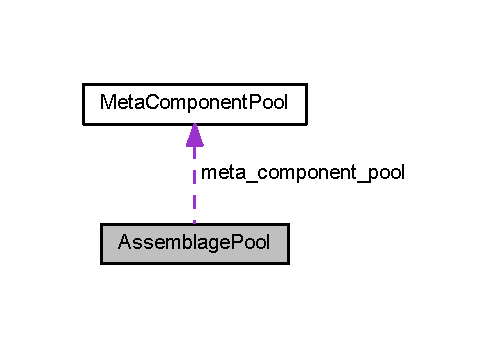
\includegraphics[width=236pt]{struct_assemblage_pool__coll__graph}
\end{center}
\end{figure}
\subsection*{Data Fields}
\begin{DoxyCompactItemize}
\item 
int \mbox{\hyperlink{struct_assemblage_pool_ae15fe47459f6c895149f5153965c7570}{assemblage\+\_\+id}} \mbox{[}\mbox{\hyperlink{assemblage_8c_a7278dc587e6d944803677e7662c25147}{A\+S\+S\+E\+M\+B\+L\+A\+G\+E\+\_\+\+P\+O\+O\+L\+\_\+\+S\+I\+ZE}}\mbox{]}
\item 
\mbox{\hyperlink{struct_meta_component_pool}{Meta\+Component\+Pool}} $\ast$ \mbox{\hyperlink{struct_assemblage_pool_a84508fb56f488124e510895704581e33}{meta\+\_\+component\+\_\+pool}} \mbox{[}\mbox{\hyperlink{assemblage_8c_a7278dc587e6d944803677e7662c25147}{A\+S\+S\+E\+M\+B\+L\+A\+G\+E\+\_\+\+P\+O\+O\+L\+\_\+\+S\+I\+ZE}}\mbox{]}
\end{DoxyCompactItemize}


\subsection{Detailed Description}
Assemblage pool. 

\subsection{Field Documentation}
\mbox{\Hypertarget{struct_assemblage_pool_ae15fe47459f6c895149f5153965c7570}\label{struct_assemblage_pool_ae15fe47459f6c895149f5153965c7570}} 
\index{Assemblage\+Pool@{Assemblage\+Pool}!assemblage\+\_\+id@{assemblage\+\_\+id}}
\index{assemblage\+\_\+id@{assemblage\+\_\+id}!Assemblage\+Pool@{Assemblage\+Pool}}
\subsubsection{\texorpdfstring{assemblage\+\_\+id}{assemblage\_id}}
{\footnotesize\ttfamily int assemblage\+\_\+id\mbox{[}\mbox{\hyperlink{assemblage_8c_a7278dc587e6d944803677e7662c25147}{A\+S\+S\+E\+M\+B\+L\+A\+G\+E\+\_\+\+P\+O\+O\+L\+\_\+\+S\+I\+ZE}}\mbox{]}}

\mbox{\Hypertarget{struct_assemblage_pool_a84508fb56f488124e510895704581e33}\label{struct_assemblage_pool_a84508fb56f488124e510895704581e33}} 
\index{Assemblage\+Pool@{Assemblage\+Pool}!meta\+\_\+component\+\_\+pool@{meta\+\_\+component\+\_\+pool}}
\index{meta\+\_\+component\+\_\+pool@{meta\+\_\+component\+\_\+pool}!Assemblage\+Pool@{Assemblage\+Pool}}
\subsubsection{\texorpdfstring{meta\+\_\+component\+\_\+pool}{meta\_component\_pool}}
{\footnotesize\ttfamily \mbox{\hyperlink{struct_meta_component_pool}{Meta\+Component\+Pool}}$\ast$ meta\+\_\+component\+\_\+pool\mbox{[}\mbox{\hyperlink{assemblage_8c_a7278dc587e6d944803677e7662c25147}{A\+S\+S\+E\+M\+B\+L\+A\+G\+E\+\_\+\+P\+O\+O\+L\+\_\+\+S\+I\+ZE}}\mbox{]}}



The documentation for this struct was generated from the following file\+:\begin{DoxyCompactItemize}
\item 
/home/drvanon/\+Documents/scripts/\+D\+E\+S/src/\mbox{\hyperlink{assemblage_8c}{assemblage.\+c}}\end{DoxyCompactItemize}

\hypertarget{struct_entity_pool}{}\section{Entity\+Pool Struct Reference}
\label{struct_entity_pool}\index{Entity\+Pool@{Entity\+Pool}}


The pool that holds the entities and component relationships.  




{\ttfamily \#include $<$des.\+h$>$}



Collaboration diagram for Entity\+Pool\+:\nopagebreak
\begin{figure}[H]
\begin{center}
\leavevmode
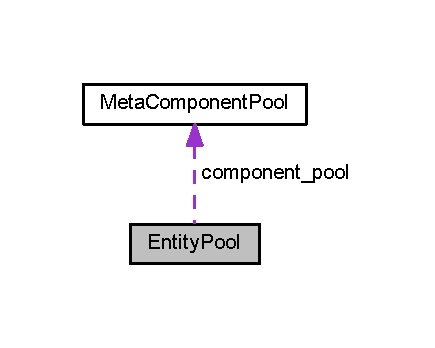
\includegraphics[width=209pt]{struct_entity_pool__coll__graph}
\end{center}
\end{figure}
\subsection*{Data Fields}
\begin{DoxyCompactItemize}
\item 
int \mbox{\hyperlink{struct_entity_pool_a439227feff9d7f55384e8780cfc2eb82}{size}}
\item 
int $\ast$ \mbox{\hyperlink{struct_entity_pool_a7ce754a177a158c41e7eae14122a3603}{guid}}
\item 
\mbox{\hyperlink{struct_meta_component_pool}{Meta\+Component\+Pool}} $\ast$$\ast$ \mbox{\hyperlink{struct_entity_pool_a9eecab6811f2cbb7343d9638605cc74d}{component\+\_\+pool}}
\item 
int $\ast$ \mbox{\hyperlink{struct_entity_pool_a2de99c265dcc7ac0f0fa20efeec9516f}{component\+\_\+index}}
\item 
int \mbox{\hyperlink{struct_entity_pool_aefadcdd88d2e6364fd584f35c374d324}{last\+G\+U\+ID}}
\end{DoxyCompactItemize}


\subsection{Detailed Description}
The pool that holds the entities and component relationships. 

\subsection{Field Documentation}
\mbox{\Hypertarget{struct_entity_pool_a2de99c265dcc7ac0f0fa20efeec9516f}\label{struct_entity_pool_a2de99c265dcc7ac0f0fa20efeec9516f}} 
\index{Entity\+Pool@{Entity\+Pool}!component\+\_\+index@{component\+\_\+index}}
\index{component\+\_\+index@{component\+\_\+index}!Entity\+Pool@{Entity\+Pool}}
\subsubsection{\texorpdfstring{component\+\_\+index}{component\_index}}
{\footnotesize\ttfamily int $\ast$ component\+\_\+index}

Index in the component pool specified in {\ttfamily component\+\_\+pool} that gives the value for this entity. \mbox{\Hypertarget{struct_entity_pool_a9eecab6811f2cbb7343d9638605cc74d}\label{struct_entity_pool_a9eecab6811f2cbb7343d9638605cc74d}} 
\index{Entity\+Pool@{Entity\+Pool}!component\+\_\+pool@{component\+\_\+pool}}
\index{component\+\_\+pool@{component\+\_\+pool}!Entity\+Pool@{Entity\+Pool}}
\subsubsection{\texorpdfstring{component\+\_\+pool}{component\_pool}}
{\footnotesize\ttfamily \mbox{\hyperlink{struct_meta_component_pool}{Meta\+Component\+Pool}} $\ast$$\ast$ component\+\_\+pool}

List of pointers to the relevant component pool \mbox{\Hypertarget{struct_entity_pool_a7ce754a177a158c41e7eae14122a3603}\label{struct_entity_pool_a7ce754a177a158c41e7eae14122a3603}} 
\index{Entity\+Pool@{Entity\+Pool}!guid@{guid}}
\index{guid@{guid}!Entity\+Pool@{Entity\+Pool}}
\subsubsection{\texorpdfstring{guid}{guid}}
{\footnotesize\ttfamily int $\ast$ guid}

Globally Unique I\+Dentifier of an identity. {\ttfamily guid\mbox{[}i\mbox{]}} represents the i-\/th entity. \mbox{\Hypertarget{struct_entity_pool_aefadcdd88d2e6364fd584f35c374d324}\label{struct_entity_pool_aefadcdd88d2e6364fd584f35c374d324}} 
\index{Entity\+Pool@{Entity\+Pool}!last\+G\+U\+ID@{last\+G\+U\+ID}}
\index{last\+G\+U\+ID@{last\+G\+U\+ID}!Entity\+Pool@{Entity\+Pool}}
\subsubsection{\texorpdfstring{last\+G\+U\+ID}{lastGUID}}
{\footnotesize\ttfamily int last\+G\+U\+ID}

Last G\+U\+ID given to an entity in this list \mbox{\Hypertarget{struct_entity_pool_a439227feff9d7f55384e8780cfc2eb82}\label{struct_entity_pool_a439227feff9d7f55384e8780cfc2eb82}} 
\index{Entity\+Pool@{Entity\+Pool}!size@{size}}
\index{size@{size}!Entity\+Pool@{Entity\+Pool}}
\subsubsection{\texorpdfstring{size}{size}}
{\footnotesize\ttfamily int size}

Amount of rows that the pool will be able to hold 

The documentation for this struct was generated from the following files\+:\begin{DoxyCompactItemize}
\item 
/home/drvanon/\+Documents/scripts/\+D\+E\+S/examples/velocity/include/\mbox{\hyperlink{examples_2velocity_2include_2des_8h}{des.\+h}}\item 
/home/drvanon/\+Documents/scripts/\+D\+E\+S/include/\mbox{\hyperlink{entity_8h}{entity.\+h}}\end{DoxyCompactItemize}

\hypertarget{struct_meta_component_pool}{}\section{Meta\+Component\+Pool Struct Reference}
\label{struct_meta_component_pool}\index{Meta\+Component\+Pool@{Meta\+Component\+Pool}}


Struct that creates a layer of abstraction between D\+ES and the user\textquotesingle{}s component pools.  




{\ttfamily \#include $<$des.\+h$>$}

\subsection*{Data Fields}
\begin{DoxyCompactItemize}
\item 
\mbox{\hyperlink{des__internal_8h_a3f7e2bcbb0b4c338f3c4f6c937cd4234}{u64}} $\ast$ \mbox{\hyperlink{struct_meta_component_pool_a43d2252901e2a4aa70563cfb707b6fa7}{mask}}
\item 
int \mbox{\hyperlink{struct_meta_component_pool_a439227feff9d7f55384e8780cfc2eb82}{size}}
\item 
void $\ast$ \mbox{\hyperlink{struct_meta_component_pool_a07582a80a343fc37057a7cc9baf4287e}{component\+\_\+pool}}
\end{DoxyCompactItemize}


\subsection{Detailed Description}
Struct that creates a layer of abstraction between D\+ES and the user\textquotesingle{}s component pools. 

\subsection{Field Documentation}
\mbox{\Hypertarget{struct_meta_component_pool_a07582a80a343fc37057a7cc9baf4287e}\label{struct_meta_component_pool_a07582a80a343fc37057a7cc9baf4287e}} 
\index{Meta\+Component\+Pool@{Meta\+Component\+Pool}!component\+\_\+pool@{component\+\_\+pool}}
\index{component\+\_\+pool@{component\+\_\+pool}!Meta\+Component\+Pool@{Meta\+Component\+Pool}}
\subsubsection{\texorpdfstring{component\+\_\+pool}{component\_pool}}
{\footnotesize\ttfamily void$\ast$ component\+\_\+pool}

Reference to the component pool \mbox{\Hypertarget{struct_meta_component_pool_a43d2252901e2a4aa70563cfb707b6fa7}\label{struct_meta_component_pool_a43d2252901e2a4aa70563cfb707b6fa7}} 
\index{Meta\+Component\+Pool@{Meta\+Component\+Pool}!mask@{mask}}
\index{mask@{mask}!Meta\+Component\+Pool@{Meta\+Component\+Pool}}
\subsubsection{\texorpdfstring{mask}{mask}}
{\footnotesize\ttfamily \mbox{\hyperlink{des__internal_8h_a3f7e2bcbb0b4c338f3c4f6c937cd4234}{u64}}$\ast$ mask}

Bitwise representation of the table. 1 means the slot/row is in use, 0 implies the row can be filled with a new entity. \mbox{\Hypertarget{struct_meta_component_pool_a439227feff9d7f55384e8780cfc2eb82}\label{struct_meta_component_pool_a439227feff9d7f55384e8780cfc2eb82}} 
\index{Meta\+Component\+Pool@{Meta\+Component\+Pool}!size@{size}}
\index{size@{size}!Meta\+Component\+Pool@{Meta\+Component\+Pool}}
\subsubsection{\texorpdfstring{size}{size}}
{\footnotesize\ttfamily int size}

Size in rows that the component pool should be able to hold. This information is supplied by the user. 

The documentation for this struct was generated from the following file\+:\begin{DoxyCompactItemize}
\item 
\mbox{\hyperlink{des_8h}{des.\+h}}\end{DoxyCompactItemize}

\hypertarget{struct_position_component_pool}{}\section{Position\+Component\+Pool Struct Reference}
\label{struct_position_component_pool}\index{Position\+Component\+Pool@{Position\+Component\+Pool}}


Component for the position of the entity.  




{\ttfamily \#include $<$components.\+h$>$}

\subsection*{Data Fields}
\begin{DoxyCompactItemize}
\item 
float $\ast$ \mbox{\hyperlink{struct_position_component_pool_af4eba642fe9ac912c7ee52aad45cdf68}{x\+\_\+position}}
\item 
float $\ast$ \mbox{\hyperlink{struct_position_component_pool_a5ea1dda60393a635fcad285a12677061}{y\+\_\+position}}
\end{DoxyCompactItemize}


\subsection{Detailed Description}
Component for the position of the entity. 

\subsection{Field Documentation}
\mbox{\Hypertarget{struct_position_component_pool_af4eba642fe9ac912c7ee52aad45cdf68}\label{struct_position_component_pool_af4eba642fe9ac912c7ee52aad45cdf68}} 
\index{Position\+Component\+Pool@{Position\+Component\+Pool}!x\+\_\+position@{x\+\_\+position}}
\index{x\+\_\+position@{x\+\_\+position}!Position\+Component\+Pool@{Position\+Component\+Pool}}
\subsubsection{\texorpdfstring{x\+\_\+position}{x\_position}}
{\footnotesize\ttfamily float$\ast$ x\+\_\+position}

\mbox{\Hypertarget{struct_position_component_pool_a5ea1dda60393a635fcad285a12677061}\label{struct_position_component_pool_a5ea1dda60393a635fcad285a12677061}} 
\index{Position\+Component\+Pool@{Position\+Component\+Pool}!y\+\_\+position@{y\+\_\+position}}
\index{y\+\_\+position@{y\+\_\+position}!Position\+Component\+Pool@{Position\+Component\+Pool}}
\subsubsection{\texorpdfstring{y\+\_\+position}{y\_position}}
{\footnotesize\ttfamily float$\ast$ y\+\_\+position}



The documentation for this struct was generated from the following file\+:\begin{DoxyCompactItemize}
\item 
components/\mbox{\hyperlink{components_8h}{components.\+h}}\end{DoxyCompactItemize}

\hypertarget{struct_test_component_pool}{}\section{Test\+Component\+Pool Struct Reference}
\label{struct_test_component_pool}\index{Test\+Component\+Pool@{Test\+Component\+Pool}}
\subsection*{Data Fields}
\begin{DoxyCompactItemize}
\item 
int $\ast$ \mbox{\hyperlink{struct_test_component_pool_a8a2b3ab64fa0522a285d284f6e365ab6}{member1}}
\item 
int $\ast$ \mbox{\hyperlink{struct_test_component_pool_a401fcf2bfe0aaaf96d646b535813c683}{member2}}
\end{DoxyCompactItemize}


\subsection{Field Documentation}
\mbox{\Hypertarget{struct_test_component_pool_a8a2b3ab64fa0522a285d284f6e365ab6}\label{struct_test_component_pool_a8a2b3ab64fa0522a285d284f6e365ab6}} 
\index{Test\+Component\+Pool@{Test\+Component\+Pool}!member1@{member1}}
\index{member1@{member1}!Test\+Component\+Pool@{Test\+Component\+Pool}}
\subsubsection{\texorpdfstring{member1}{member1}}
{\footnotesize\ttfamily int$\ast$ member1}

\mbox{\Hypertarget{struct_test_component_pool_a401fcf2bfe0aaaf96d646b535813c683}\label{struct_test_component_pool_a401fcf2bfe0aaaf96d646b535813c683}} 
\index{Test\+Component\+Pool@{Test\+Component\+Pool}!member2@{member2}}
\index{member2@{member2}!Test\+Component\+Pool@{Test\+Component\+Pool}}
\subsubsection{\texorpdfstring{member2}{member2}}
{\footnotesize\ttfamily int$\ast$ member2}



The documentation for this struct was generated from the following file\+:\begin{DoxyCompactItemize}
\item 
/home/drvanon/\+Documents/scripts/\+D\+E\+S/tests/\mbox{\hyperlink{test_8c}{test.\+c}}\end{DoxyCompactItemize}

\hypertarget{struct_velocity_component_pool}{}\section{Velocity\+Component\+Pool Struct Reference}
\label{struct_velocity_component_pool}\index{Velocity\+Component\+Pool@{Velocity\+Component\+Pool}}


Component with the velocity data. This gets added to the position by a system.  




{\ttfamily \#include $<$components.\+h$>$}

\subsection*{Data Fields}
\begin{DoxyCompactItemize}
\item 
float $\ast$ \mbox{\hyperlink{struct_velocity_component_pool_a894c40834929b9d5f24377c2c4308432}{x\+\_\+velocity}}
\item 
float $\ast$ \mbox{\hyperlink{struct_velocity_component_pool_aaf5dda6f5c06e80a111272ce1fe7b208}{y\+\_\+velocity}}
\end{DoxyCompactItemize}


\subsection{Detailed Description}
Component with the velocity data. This gets added to the position by a system. 

\subsection{Field Documentation}
\mbox{\Hypertarget{struct_velocity_component_pool_a894c40834929b9d5f24377c2c4308432}\label{struct_velocity_component_pool_a894c40834929b9d5f24377c2c4308432}} 
\index{Velocity\+Component\+Pool@{Velocity\+Component\+Pool}!x\+\_\+velocity@{x\+\_\+velocity}}
\index{x\+\_\+velocity@{x\+\_\+velocity}!Velocity\+Component\+Pool@{Velocity\+Component\+Pool}}
\subsubsection{\texorpdfstring{x\+\_\+velocity}{x\_velocity}}
{\footnotesize\ttfamily float$\ast$ x\+\_\+velocity}

\mbox{\Hypertarget{struct_velocity_component_pool_aaf5dda6f5c06e80a111272ce1fe7b208}\label{struct_velocity_component_pool_aaf5dda6f5c06e80a111272ce1fe7b208}} 
\index{Velocity\+Component\+Pool@{Velocity\+Component\+Pool}!y\+\_\+velocity@{y\+\_\+velocity}}
\index{y\+\_\+velocity@{y\+\_\+velocity}!Velocity\+Component\+Pool@{Velocity\+Component\+Pool}}
\subsubsection{\texorpdfstring{y\+\_\+velocity}{y\_velocity}}
{\footnotesize\ttfamily float$\ast$ y\+\_\+velocity}



The documentation for this struct was generated from the following file\+:\begin{DoxyCompactItemize}
\item 
/home/drvanon/\+Documents/scripts/\+D\+E\+S/examples/velocity/src/components/\mbox{\hyperlink{components_8h}{components.\+h}}\end{DoxyCompactItemize}

\chapter{File Documentation}
\hypertarget{examples_2velocity_2include_2des_8h}{}\section{/home/drvanon/\+Documents/scripts/\+D\+E\+S/examples/velocity/include/des.h File Reference}
\label{examples_2velocity_2include_2des_8h}\index{/home/drvanon/\+Documents/scripts/\+D\+E\+S/examples/velocity/include/des.\+h@{/home/drvanon/\+Documents/scripts/\+D\+E\+S/examples/velocity/include/des.\+h}}
{\ttfamily \#include \char`\"{}des\+\_\+internal.\+h\char`\"{}}\newline
Include dependency graph for des.\+h\+:\nopagebreak
\begin{figure}[H]
\begin{center}
\leavevmode
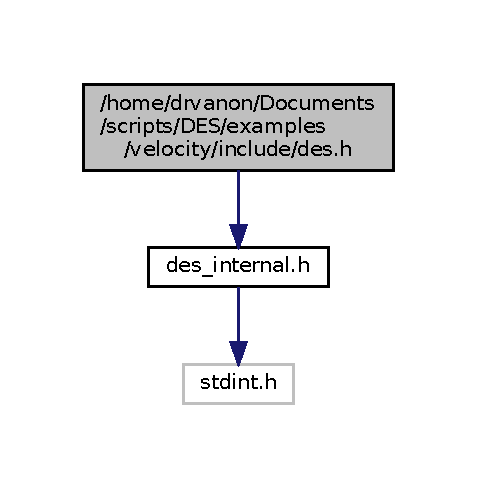
\includegraphics[width=229pt]{examples_2velocity_2include_2des_8h__incl}
\end{center}
\end{figure}
\subsection*{Data Structures}
\begin{DoxyCompactItemize}
\item 
struct \mbox{\hyperlink{struct_meta_component_pool}{Meta\+Component\+Pool}}
\begin{DoxyCompactList}\small\item\em Struct that creates a layer of abstraction between D\+ES and the user\textquotesingle{}s component pools. \end{DoxyCompactList}\item 
struct \mbox{\hyperlink{struct_entity_pool}{Entity\+Pool}}
\begin{DoxyCompactList}\small\item\em The pool that holds the entities and component relationships. \end{DoxyCompactList}\end{DoxyCompactItemize}
\subsection*{Typedefs}
\begin{DoxyCompactItemize}
\item 
typedef struct \mbox{\hyperlink{struct_meta_component_pool}{Meta\+Component\+Pool}} \mbox{\hyperlink{examples_2velocity_2include_2des_8h_a0a09b6ff207d87cced8d3f986a50a101}{Meta\+Component\+Pool}}
\begin{DoxyCompactList}\small\item\em Struct that creates a layer of abstraction between D\+ES and the user\textquotesingle{}s component pools. \end{DoxyCompactList}\item 
typedef struct \mbox{\hyperlink{struct_entity_pool}{Entity\+Pool}} \mbox{\hyperlink{examples_2velocity_2include_2des_8h_a629511a19dc302aaada724794387569d}{Entity\+Pool}}
\begin{DoxyCompactList}\small\item\em The pool that holds the entities and component relationships. \end{DoxyCompactList}\end{DoxyCompactItemize}
\subsection*{Functions}
\begin{DoxyCompactItemize}
\item 
\mbox{\hyperlink{struct_entity_pool}{Entity\+Pool}} $\ast$ \mbox{\hyperlink{examples_2velocity_2include_2des_8h_a44b8855c1b56396b8faedcd389fe4546}{entity\+\_\+pool\+\_\+create}} (int size)
\begin{DoxyCompactList}\small\item\em Create \mbox{\hyperlink{struct_entity_pool}{Entity\+Pool}} and malloc it\textquotesingle{}s component with the size provided, returns N\+U\+LL if insufficient R\+AM. \end{DoxyCompactList}\item 
void \mbox{\hyperlink{examples_2velocity_2include_2des_8h_a3e377867fe9b332352eb47cdf9dc1a4c}{entity\+\_\+pool\+\_\+destroy}} (\mbox{\hyperlink{struct_entity_pool}{Entity\+Pool}} $\ast$entity\+\_\+pool)
\begin{DoxyCompactList}\small\item\em Free all memory allocated for the \mbox{\hyperlink{struct_entity_pool}{Entity\+Pool}}. \end{DoxyCompactList}\item 
int \mbox{\hyperlink{examples_2velocity_2include_2des_8h_a3955b16f45429c7ea74f275dac36493d}{entity\+\_\+pool\+\_\+find\+\_\+empty\+\_\+row}} (\mbox{\hyperlink{struct_entity_pool}{Entity\+Pool}} $\ast$entity\+\_\+pool)
\begin{DoxyCompactList}\small\item\em Find the index first empty row in the provided \mbox{\hyperlink{struct_entity_pool}{Entity\+Pool}}. \end{DoxyCompactList}\item 
int \mbox{\hyperlink{examples_2velocity_2include_2des_8h_ae84c376a8fb9ccf53cd54e0736e76eb2}{entity\+\_\+create}} (\mbox{\hyperlink{struct_entity_pool}{Entity\+Pool}} $\ast$entity\+\_\+pool)
\begin{DoxyCompactList}\small\item\em Retrieve a new guid for an entity and register the change. \end{DoxyCompactList}\item 
void \mbox{\hyperlink{examples_2velocity_2include_2des_8h_a7fa6d71c51a14d7607b66722a1f17427}{entity\+\_\+remove}} (\mbox{\hyperlink{struct_entity_pool}{Entity\+Pool}} $\ast$entity\+\_\+pool, int guid)
\begin{DoxyCompactList}\small\item\em Remove all data on the entity in the provided \mbox{\hyperlink{struct_entity_pool}{Entity\+Pool}}. \end{DoxyCompactList}\item 
\mbox{\hyperlink{struct_entity_pool}{Entity\+Pool}} $\ast$ \mbox{\hyperlink{examples_2velocity_2include_2des_8h_a67e67b5444435172378a5e24701a02e7}{entity\+\_\+get\+\_\+components}} (\mbox{\hyperlink{struct_entity_pool}{Entity\+Pool}} $\ast$entity\+\_\+pool, int guid, int max\+\_\+query\+\_\+size)
\begin{DoxyCompactList}\small\item\em Retrieve upto max\+\_\+query\+\_\+size components linked to the entity in an \mbox{\hyperlink{struct_entity_pool}{Entity\+Pool}}. \end{DoxyCompactList}\item 
\mbox{\hyperlink{struct_meta_component_pool}{Meta\+Component\+Pool}} \mbox{\hyperlink{examples_2velocity_2include_2des_8h_ac9e98c2d8d4ef8d84bda94d824fbc7b0}{component\+\_\+pool\+\_\+register}} (void $\ast$component\+\_\+pool, int size)
\begin{DoxyCompactList}\small\item\em Register a component for use in the D\+ES system. \end{DoxyCompactList}\item 
int \mbox{\hyperlink{examples_2velocity_2include_2des_8h_a45e8d15e4080e8fb930e984fc9bac47a}{component\+\_\+add\+\_\+to\+\_\+entity\+\_\+\+ID}} (\mbox{\hyperlink{struct_entity_pool}{Entity\+Pool}} $\ast$entity\+\_\+pool, int guid, \mbox{\hyperlink{struct_meta_component_pool}{Meta\+Component\+Pool}} $\ast$meta\+\_\+component\+\_\+pool)
\begin{DoxyCompactList}\small\item\em Create a new row in the component-\/entity pool. \end{DoxyCompactList}\item 
int \mbox{\hyperlink{examples_2velocity_2include_2des_8h_a494f2d263a1053e2962e158f0a4c7e3a}{component\+\_\+add\+\_\+to\+\_\+entity\+\_\+index}} (\mbox{\hyperlink{struct_entity_pool}{Entity\+Pool}} $\ast$entity\+\_\+pool, int index, int guid, \mbox{\hyperlink{struct_meta_component_pool}{Meta\+Component\+Pool}} $\ast$meta\+\_\+component\+\_\+pool)
\begin{DoxyCompactList}\small\item\em Add a component to an entity if the user has already obtained an empty row. \end{DoxyCompactList}\item 
int \mbox{\hyperlink{examples_2velocity_2include_2des_8h_a46ad35b10ce23dc588b43f20fa5be2c2}{component\+\_\+remove\+\_\+from\+\_\+entity\+\_\+index}} (\mbox{\hyperlink{struct_entity_pool}{Entity\+Pool}} $\ast$entity\+\_\+pool, int index)
\begin{DoxyCompactList}\small\item\em Remove the row of the given index in the component-\/entity pool. \end{DoxyCompactList}\item 
int \mbox{\hyperlink{examples_2velocity_2include_2des_8h_af64e2220dd5596ce4f119c7887eac5c0}{component\+\_\+remove\+\_\+from\+\_\+entity\+\_\+\+ID}} (\mbox{\hyperlink{struct_entity_pool}{Entity\+Pool}} $\ast$entity\+\_\+pool, int guid, \mbox{\hyperlink{struct_meta_component_pool}{Meta\+Component\+Pool}} $\ast$meta\+\_\+component\+\_\+pool)
\begin{DoxyCompactList}\small\item\em Remove a single component from the specified entity. \end{DoxyCompactList}\item 
int \mbox{\hyperlink{examples_2velocity_2include_2des_8h_a997d5c45b99e95e34d3d00107eec6618}{component\+\_\+pool\+\_\+get\+\_\+open\+\_\+slot}} (\mbox{\hyperlink{struct_meta_component_pool}{Meta\+Component\+Pool}} $\ast$meta\+\_\+component\+\_\+pool)
\begin{DoxyCompactList}\small\item\em Find the first slot in the mask that has not been filled. \end{DoxyCompactList}\item 
int \mbox{\hyperlink{examples_2velocity_2include_2des_8h_a882c82b33bb428b62dab1b01c37e12a2}{component\+\_\+pool\+\_\+get\+\_\+slot}} (\mbox{\hyperlink{struct_meta_component_pool}{Meta\+Component\+Pool}} $\ast$meta\+\_\+component\+\_\+pool, int index)
\begin{DoxyCompactList}\small\item\em Find the state of a slot in a component pool. \end{DoxyCompactList}\item 
int \mbox{\hyperlink{examples_2velocity_2include_2des_8h_a1092fc1b1a8b8c021bc8e9dca328cf6c}{component\+\_\+pool\+\_\+set\+\_\+slot}} (\mbox{\hyperlink{struct_meta_component_pool}{Meta\+Component\+Pool}} $\ast$meta\+\_\+component\+\_\+pool, int index, int state)
\begin{DoxyCompactList}\small\item\em Set slot state in meta component to be vacant or free. \end{DoxyCompactList}\end{DoxyCompactItemize}


\subsection{Typedef Documentation}
\mbox{\Hypertarget{examples_2velocity_2include_2des_8h_a629511a19dc302aaada724794387569d}\label{examples_2velocity_2include_2des_8h_a629511a19dc302aaada724794387569d}} 
\index{examples/velocity/include/des.\+h@{examples/velocity/include/des.\+h}!Entity\+Pool@{Entity\+Pool}}
\index{Entity\+Pool@{Entity\+Pool}!examples/velocity/include/des.\+h@{examples/velocity/include/des.\+h}}
\subsubsection{\texorpdfstring{Entity\+Pool}{EntityPool}}
{\footnotesize\ttfamily typedef struct \mbox{\hyperlink{struct_entity_pool}{Entity\+Pool}}  \mbox{\hyperlink{struct_entity_pool}{Entity\+Pool}}}



The pool that holds the entities and component relationships. 

\mbox{\Hypertarget{examples_2velocity_2include_2des_8h_a0a09b6ff207d87cced8d3f986a50a101}\label{examples_2velocity_2include_2des_8h_a0a09b6ff207d87cced8d3f986a50a101}} 
\index{examples/velocity/include/des.\+h@{examples/velocity/include/des.\+h}!Meta\+Component\+Pool@{Meta\+Component\+Pool}}
\index{Meta\+Component\+Pool@{Meta\+Component\+Pool}!examples/velocity/include/des.\+h@{examples/velocity/include/des.\+h}}
\subsubsection{\texorpdfstring{Meta\+Component\+Pool}{MetaComponentPool}}
{\footnotesize\ttfamily typedef struct \mbox{\hyperlink{struct_meta_component_pool}{Meta\+Component\+Pool}}  \mbox{\hyperlink{struct_meta_component_pool}{Meta\+Component\+Pool}}}



Struct that creates a layer of abstraction between D\+ES and the user\textquotesingle{}s component pools. 



\subsection{Function Documentation}
\mbox{\Hypertarget{examples_2velocity_2include_2des_8h_a45e8d15e4080e8fb930e984fc9bac47a}\label{examples_2velocity_2include_2des_8h_a45e8d15e4080e8fb930e984fc9bac47a}} 
\index{examples/velocity/include/des.\+h@{examples/velocity/include/des.\+h}!component\+\_\+add\+\_\+to\+\_\+entity\+\_\+\+ID@{component\+\_\+add\+\_\+to\+\_\+entity\+\_\+\+ID}}
\index{component\+\_\+add\+\_\+to\+\_\+entity\+\_\+\+ID@{component\+\_\+add\+\_\+to\+\_\+entity\+\_\+\+ID}!examples/velocity/include/des.\+h@{examples/velocity/include/des.\+h}}
\subsubsection{\texorpdfstring{component\+\_\+add\+\_\+to\+\_\+entity\+\_\+\+I\+D()}{component\_add\_to\_entity\_ID()}}
{\footnotesize\ttfamily int component\+\_\+add\+\_\+to\+\_\+entity\+\_\+\+ID (\begin{DoxyParamCaption}\item[{\mbox{\hyperlink{struct_entity_pool}{Entity\+Pool}} $\ast$}]{entity\+\_\+pool,  }\item[{int}]{guid,  }\item[{\mbox{\hyperlink{struct_meta_component_pool}{Meta\+Component\+Pool}} $\ast$}]{meta\+\_\+component\+\_\+pool }\end{DoxyParamCaption})}



Create a new row in the component-\/entity pool. 

This function takes a previously established G\+U\+ID and a \mbox{\hyperlink{struct_meta_component_pool}{Meta\+Component\+Pool}} to create a new row in the component-\/entity pool. This is to be used in combination with create\+Entity, after having registered your component. 
\begin{DoxyCode}
\textcolor{keywordtype}{int} your\_component\_pool\_size = 200; \textcolor{comment}{// Amount of rows the componentPool can have}
EnityPool *entity\_pool = \mbox{\hyperlink{examples_2velocity_2include_2des_8h_a44b8855c1b56396b8faedcd389fe4546}{entity\_pool\_create}}(2000);
MetaComponentPoolPool YourMetaComponentPoolPool = component\_register(entity\_pool, *YourComponentPool, 
      your\_component\_pool\_size);
\textcolor{keywordtype}{int} guid = \mbox{\hyperlink{examples_2velocity_2include_2des_8h_ae84c376a8fb9ccf53cd54e0736e76eb2}{entity\_create}}();
\textcolor{keywordtype}{int} component\_index = \mbox{\hyperlink{examples_2velocity_2include_2des_8h_a45e8d15e4080e8fb930e984fc9bac47a}{component\_add\_to\_entity\_ID}}(guid, &YourMetaComponentPoolPool
      );
YourComponentPool.member1[component\_index] = \textcolor{stringliteral}{"Some content"};

\textcolor{comment}{// And after running the program:}
\mbox{\hyperlink{examples_2velocity_2include_2des_8h_a3e377867fe9b332352eb47cdf9dc1a4c}{entity\_pool\_destroy}}(entity\_pool);
free(YourComponent.member1);
free(YourComponent.member2); \textcolor{comment}{// etc.}
\end{DoxyCode}



\begin{DoxyParams}{Parameters}
{\em entity\+\_\+pool} & \\
\hline
{\em guid} & \\
\hline
{\em meta\+\_\+component\+\_\+pool} & \\
\hline
\end{DoxyParams}
\begin{DoxyReturn}{Returns}
int This variable refers to the index of the user defined component pool that can be set to the prefered data, see example above. 
\end{DoxyReturn}
Here is the caller graph for this function\+:\nopagebreak
\begin{figure}[H]
\begin{center}
\leavevmode
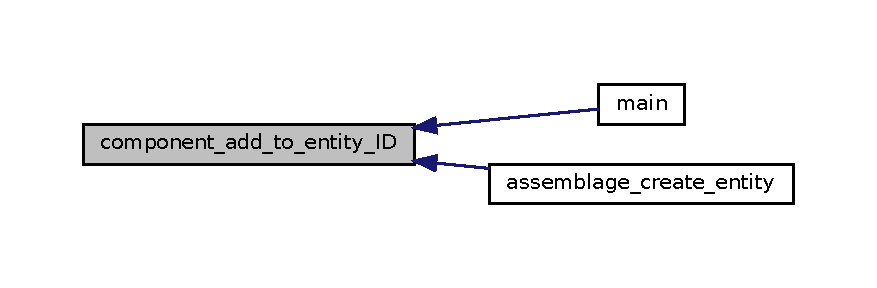
\includegraphics[width=350pt]{examples_2velocity_2include_2des_8h_a45e8d15e4080e8fb930e984fc9bac47a_icgraph}
\end{center}
\end{figure}
\mbox{\Hypertarget{examples_2velocity_2include_2des_8h_a494f2d263a1053e2962e158f0a4c7e3a}\label{examples_2velocity_2include_2des_8h_a494f2d263a1053e2962e158f0a4c7e3a}} 
\index{examples/velocity/include/des.\+h@{examples/velocity/include/des.\+h}!component\+\_\+add\+\_\+to\+\_\+entity\+\_\+index@{component\+\_\+add\+\_\+to\+\_\+entity\+\_\+index}}
\index{component\+\_\+add\+\_\+to\+\_\+entity\+\_\+index@{component\+\_\+add\+\_\+to\+\_\+entity\+\_\+index}!examples/velocity/include/des.\+h@{examples/velocity/include/des.\+h}}
\subsubsection{\texorpdfstring{component\+\_\+add\+\_\+to\+\_\+entity\+\_\+index()}{component\_add\_to\_entity\_index()}}
{\footnotesize\ttfamily int component\+\_\+add\+\_\+to\+\_\+entity\+\_\+index (\begin{DoxyParamCaption}\item[{\mbox{\hyperlink{struct_entity_pool}{Entity\+Pool}} $\ast$}]{entity\+\_\+pool,  }\item[{int}]{index,  }\item[{int}]{guid,  }\item[{\mbox{\hyperlink{struct_meta_component_pool}{Meta\+Component\+Pool}} $\ast$}]{meta\+\_\+component\+\_\+pool }\end{DoxyParamCaption})}



Add a component to an entity if the user has already obtained an empty row. 

It is possible that the user will be aware of the row that the entity was created in, so this is a copy of add\+\_\+component\+\_\+to\+\_\+entity\+\_\+\+ID, but works based of index instead of id, which is much faster, for we will not have to go trough the entire entity pool. An example for this might be inplace replacement of a row.


\begin{DoxyParams}{Parameters}
{\em entity\+\_\+pool} & \mbox{\hyperlink{struct_entity_pool}{Entity\+Pool}} in which to perform the action. \\
\hline
{\em index} & index of the entity-\/component pool \\
\hline
{\em guid} & guid of the new entity \\
\hline
{\em meta\+\_\+component\+\_\+pool} & \mbox{\hyperlink{struct_meta_component_pool}{Meta\+Component\+Pool}} of the component that is to be added to the entity \\
\hline
\end{DoxyParams}
\begin{DoxyReturn}{Returns}
int Index of component pool that can be used to store the data the user wants to store 
\end{DoxyReturn}
\mbox{\Hypertarget{examples_2velocity_2include_2des_8h_a997d5c45b99e95e34d3d00107eec6618}\label{examples_2velocity_2include_2des_8h_a997d5c45b99e95e34d3d00107eec6618}} 
\index{examples/velocity/include/des.\+h@{examples/velocity/include/des.\+h}!component\+\_\+pool\+\_\+get\+\_\+open\+\_\+slot@{component\+\_\+pool\+\_\+get\+\_\+open\+\_\+slot}}
\index{component\+\_\+pool\+\_\+get\+\_\+open\+\_\+slot@{component\+\_\+pool\+\_\+get\+\_\+open\+\_\+slot}!examples/velocity/include/des.\+h@{examples/velocity/include/des.\+h}}
\subsubsection{\texorpdfstring{component\+\_\+pool\+\_\+get\+\_\+open\+\_\+slot()}{component\_pool\_get\_open\_slot()}}
{\footnotesize\ttfamily int component\+\_\+pool\+\_\+get\+\_\+open\+\_\+slot (\begin{DoxyParamCaption}\item[{\mbox{\hyperlink{struct_meta_component_pool}{Meta\+Component\+Pool}} $\ast$}]{meta\+\_\+component\+\_\+pool }\end{DoxyParamCaption})}



Find the first slot in the mask that has not been filled. 


\begin{DoxyParams}{Parameters}
{\em meta\+\_\+component\+\_\+pool} & \\
\hline
\end{DoxyParams}
\begin{DoxyReturn}{Returns}
int component index of the open slot. 
\end{DoxyReturn}
Here is the caller graph for this function\+:\nopagebreak
\begin{figure}[H]
\begin{center}
\leavevmode
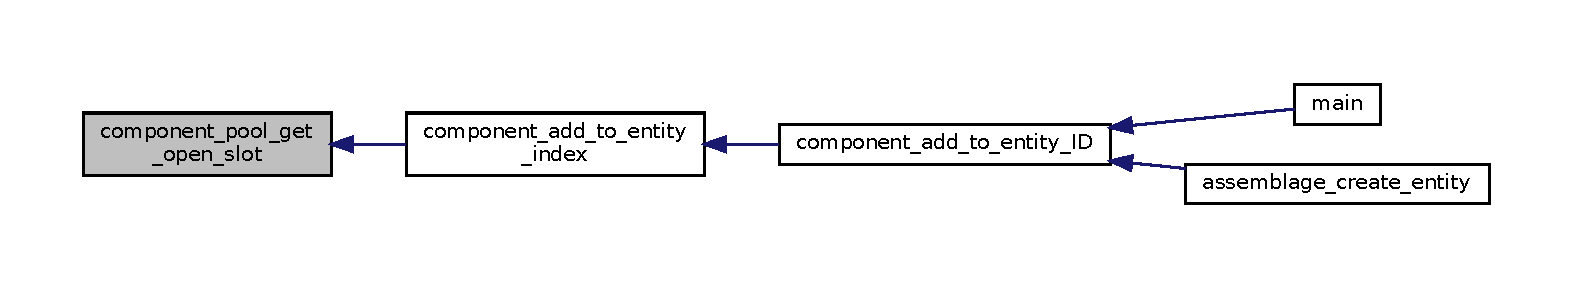
\includegraphics[width=350pt]{examples_2velocity_2include_2des_8h_a997d5c45b99e95e34d3d00107eec6618_icgraph}
\end{center}
\end{figure}
\mbox{\Hypertarget{examples_2velocity_2include_2des_8h_a882c82b33bb428b62dab1b01c37e12a2}\label{examples_2velocity_2include_2des_8h_a882c82b33bb428b62dab1b01c37e12a2}} 
\index{examples/velocity/include/des.\+h@{examples/velocity/include/des.\+h}!component\+\_\+pool\+\_\+get\+\_\+slot@{component\+\_\+pool\+\_\+get\+\_\+slot}}
\index{component\+\_\+pool\+\_\+get\+\_\+slot@{component\+\_\+pool\+\_\+get\+\_\+slot}!examples/velocity/include/des.\+h@{examples/velocity/include/des.\+h}}
\subsubsection{\texorpdfstring{component\+\_\+pool\+\_\+get\+\_\+slot()}{component\_pool\_get\_slot()}}
{\footnotesize\ttfamily int component\+\_\+pool\+\_\+get\+\_\+slot (\begin{DoxyParamCaption}\item[{\mbox{\hyperlink{struct_meta_component_pool}{Meta\+Component\+Pool}} $\ast$}]{meta\+\_\+component\+\_\+pool,  }\item[{int}]{index }\end{DoxyParamCaption})}



Find the state of a slot in a component pool. 

This function will tell the user if the slot is in vacant or not.


\begin{DoxyParams}{Parameters}
{\em meta\+\_\+component\+\_\+pool} & \\
\hline
{\em index} & \\
\hline
\end{DoxyParams}
\begin{DoxyReturn}{Returns}
int bool value 
\end{DoxyReturn}
\mbox{\Hypertarget{examples_2velocity_2include_2des_8h_ac9e98c2d8d4ef8d84bda94d824fbc7b0}\label{examples_2velocity_2include_2des_8h_ac9e98c2d8d4ef8d84bda94d824fbc7b0}} 
\index{examples/velocity/include/des.\+h@{examples/velocity/include/des.\+h}!component\+\_\+pool\+\_\+register@{component\+\_\+pool\+\_\+register}}
\index{component\+\_\+pool\+\_\+register@{component\+\_\+pool\+\_\+register}!examples/velocity/include/des.\+h@{examples/velocity/include/des.\+h}}
\subsubsection{\texorpdfstring{component\+\_\+pool\+\_\+register()}{component\_pool\_register()}}
{\footnotesize\ttfamily \mbox{\hyperlink{struct_meta_component_pool}{Meta\+Component\+Pool}} component\+\_\+pool\+\_\+register (\begin{DoxyParamCaption}\item[{void $\ast$}]{component\+\_\+pool,  }\item[{int}]{size }\end{DoxyParamCaption})}



Register a component for use in the D\+ES system. 

The \mbox{\hyperlink{struct_meta_component_pool}{Meta\+Component\+Pool}} is used to provide an abstraction layer between the D\+ES and the user. It provides information on what index of the user defined component pool is open and what row is already in use by an entity. It also gives information on the size of the pool and refers to the component pool.


\begin{DoxyParams}{Parameters}
{\em component\+\_\+pool} & Pointer to the user-\/defined component\+\_\+pool. \\
\hline
{\em size} & Size of the memory allocated for the pools. \\
\hline
\end{DoxyParams}
\begin{DoxyReturn}{Returns}
\mbox{\hyperlink{struct_meta_component_pool}{Meta\+Component\+Pool}} 
\end{DoxyReturn}
Here is the caller graph for this function\+:\nopagebreak
\begin{figure}[H]
\begin{center}
\leavevmode
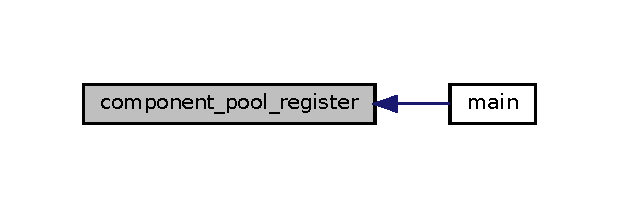
\includegraphics[width=297pt]{examples_2velocity_2include_2des_8h_ac9e98c2d8d4ef8d84bda94d824fbc7b0_icgraph}
\end{center}
\end{figure}
\mbox{\Hypertarget{examples_2velocity_2include_2des_8h_a1092fc1b1a8b8c021bc8e9dca328cf6c}\label{examples_2velocity_2include_2des_8h_a1092fc1b1a8b8c021bc8e9dca328cf6c}} 
\index{examples/velocity/include/des.\+h@{examples/velocity/include/des.\+h}!component\+\_\+pool\+\_\+set\+\_\+slot@{component\+\_\+pool\+\_\+set\+\_\+slot}}
\index{component\+\_\+pool\+\_\+set\+\_\+slot@{component\+\_\+pool\+\_\+set\+\_\+slot}!examples/velocity/include/des.\+h@{examples/velocity/include/des.\+h}}
\subsubsection{\texorpdfstring{component\+\_\+pool\+\_\+set\+\_\+slot()}{component\_pool\_set\_slot()}}
{\footnotesize\ttfamily int component\+\_\+pool\+\_\+set\+\_\+slot (\begin{DoxyParamCaption}\item[{\mbox{\hyperlink{struct_meta_component_pool}{Meta\+Component\+Pool}} $\ast$}]{meta\+\_\+component\+\_\+pool,  }\item[{int}]{index,  }\item[{int}]{state }\end{DoxyParamCaption})}



Set slot state in meta component to be vacant or free. 


\begin{DoxyParams}{Parameters}
{\em meta\+\_\+component\+\_\+pool} & Meta of the component pool \\
\hline
{\em index} & Index of the slot \\
\hline
{\em state} & Desired state of the slot \\
\hline
\end{DoxyParams}
\begin{DoxyReturn}{Returns}
int Error codes\+: 0 is okay, -\/1 is index out of bounds 
\end{DoxyReturn}
Here is the caller graph for this function\+:\nopagebreak
\begin{figure}[H]
\begin{center}
\leavevmode
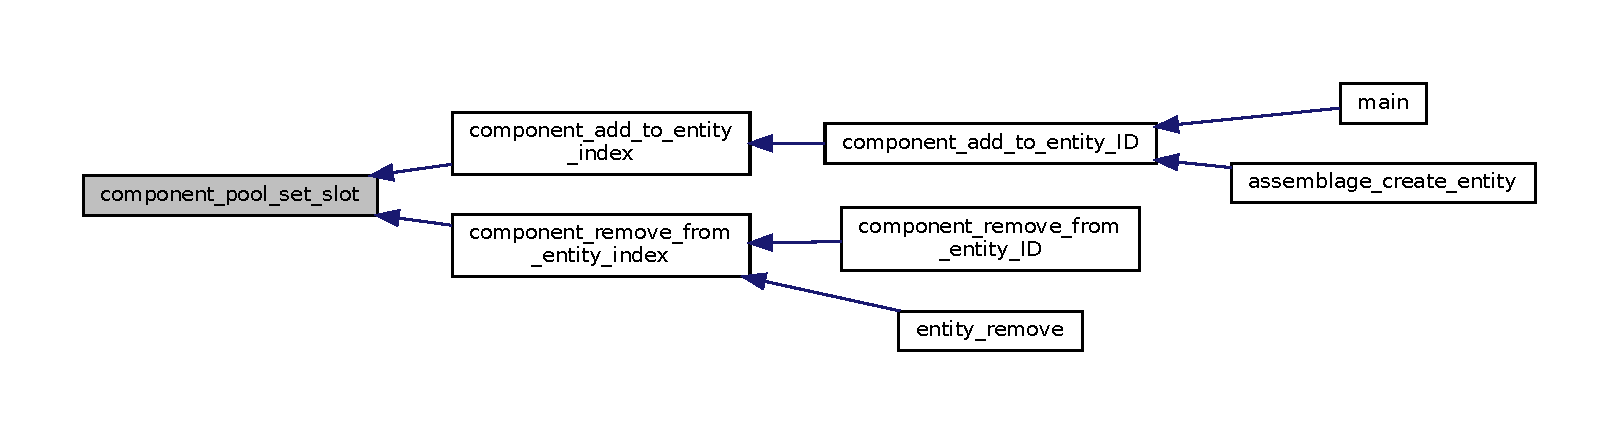
\includegraphics[width=350pt]{examples_2velocity_2include_2des_8h_a1092fc1b1a8b8c021bc8e9dca328cf6c_icgraph}
\end{center}
\end{figure}
\mbox{\Hypertarget{examples_2velocity_2include_2des_8h_af64e2220dd5596ce4f119c7887eac5c0}\label{examples_2velocity_2include_2des_8h_af64e2220dd5596ce4f119c7887eac5c0}} 
\index{examples/velocity/include/des.\+h@{examples/velocity/include/des.\+h}!component\+\_\+remove\+\_\+from\+\_\+entity\+\_\+\+ID@{component\+\_\+remove\+\_\+from\+\_\+entity\+\_\+\+ID}}
\index{component\+\_\+remove\+\_\+from\+\_\+entity\+\_\+\+ID@{component\+\_\+remove\+\_\+from\+\_\+entity\+\_\+\+ID}!examples/velocity/include/des.\+h@{examples/velocity/include/des.\+h}}
\subsubsection{\texorpdfstring{component\+\_\+remove\+\_\+from\+\_\+entity\+\_\+\+I\+D()}{component\_remove\_from\_entity\_ID()}}
{\footnotesize\ttfamily int component\+\_\+remove\+\_\+from\+\_\+entity\+\_\+\+ID (\begin{DoxyParamCaption}\item[{\mbox{\hyperlink{struct_entity_pool}{Entity\+Pool}} $\ast$}]{entity\+\_\+pool,  }\item[{int}]{guid,  }\item[{\mbox{\hyperlink{struct_meta_component_pool}{Meta\+Component\+Pool}} $\ast$}]{meta\+\_\+component\+\_\+pool }\end{DoxyParamCaption})}



Remove a single component from the specified entity. 


\begin{DoxyParams}{Parameters}
{\em entity\+\_\+pool} & \\
\hline
{\em guid} & \\
\hline
{\em meta\+\_\+component\+\_\+pool} & \\
\hline
\end{DoxyParams}
\begin{DoxyReturn}{Returns}
int Error codes\+: 0 is okay, -\/1 means could not find entity-\/component in pool. 
\end{DoxyReturn}
\mbox{\Hypertarget{examples_2velocity_2include_2des_8h_a46ad35b10ce23dc588b43f20fa5be2c2}\label{examples_2velocity_2include_2des_8h_a46ad35b10ce23dc588b43f20fa5be2c2}} 
\index{examples/velocity/include/des.\+h@{examples/velocity/include/des.\+h}!component\+\_\+remove\+\_\+from\+\_\+entity\+\_\+index@{component\+\_\+remove\+\_\+from\+\_\+entity\+\_\+index}}
\index{component\+\_\+remove\+\_\+from\+\_\+entity\+\_\+index@{component\+\_\+remove\+\_\+from\+\_\+entity\+\_\+index}!examples/velocity/include/des.\+h@{examples/velocity/include/des.\+h}}
\subsubsection{\texorpdfstring{component\+\_\+remove\+\_\+from\+\_\+entity\+\_\+index()}{component\_remove\_from\_entity\_index()}}
{\footnotesize\ttfamily int component\+\_\+remove\+\_\+from\+\_\+entity\+\_\+index (\begin{DoxyParamCaption}\item[{\mbox{\hyperlink{struct_entity_pool}{Entity\+Pool}} $\ast$}]{entity\+\_\+pool,  }\item[{int}]{index }\end{DoxyParamCaption})}



Remove the row of the given index in the component-\/entity pool. 


\begin{DoxyParams}{Parameters}
{\em entity\+\_\+pool} & \\
\hline
{\em index} & \\
\hline
\end{DoxyParams}
\begin{DoxyReturn}{Returns}
int Error codes\+: 0 is okay, -\/1 is index out of bounds 
\end{DoxyReturn}
\mbox{\Hypertarget{examples_2velocity_2include_2des_8h_ae84c376a8fb9ccf53cd54e0736e76eb2}\label{examples_2velocity_2include_2des_8h_ae84c376a8fb9ccf53cd54e0736e76eb2}} 
\index{examples/velocity/include/des.\+h@{examples/velocity/include/des.\+h}!entity\+\_\+create@{entity\+\_\+create}}
\index{entity\+\_\+create@{entity\+\_\+create}!examples/velocity/include/des.\+h@{examples/velocity/include/des.\+h}}
\subsubsection{\texorpdfstring{entity\+\_\+create()}{entity\_create()}}
{\footnotesize\ttfamily int entity\+\_\+create (\begin{DoxyParamCaption}\item[{\mbox{\hyperlink{struct_entity_pool}{Entity\+Pool}} $\ast$}]{entity\+\_\+pool }\end{DoxyParamCaption})}



Retrieve a new guid for an entity and register the change. 


\begin{DoxyParams}{Parameters}
{\em entity\+\_\+pool} & \\
\hline
\end{DoxyParams}
\begin{DoxyReturn}{Returns}
int 
\end{DoxyReturn}
Here is the caller graph for this function\+:\nopagebreak
\begin{figure}[H]
\begin{center}
\leavevmode
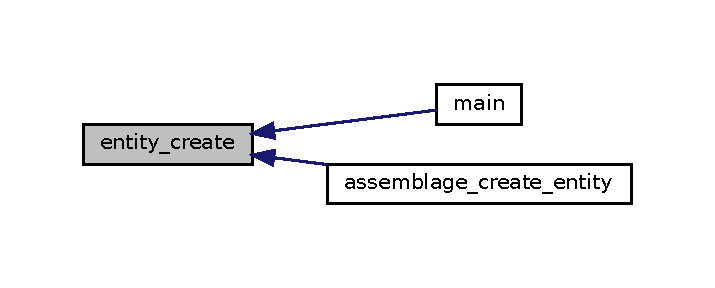
\includegraphics[width=343pt]{examples_2velocity_2include_2des_8h_ae84c376a8fb9ccf53cd54e0736e76eb2_icgraph}
\end{center}
\end{figure}
\mbox{\Hypertarget{examples_2velocity_2include_2des_8h_a67e67b5444435172378a5e24701a02e7}\label{examples_2velocity_2include_2des_8h_a67e67b5444435172378a5e24701a02e7}} 
\index{examples/velocity/include/des.\+h@{examples/velocity/include/des.\+h}!entity\+\_\+get\+\_\+components@{entity\+\_\+get\+\_\+components}}
\index{entity\+\_\+get\+\_\+components@{entity\+\_\+get\+\_\+components}!examples/velocity/include/des.\+h@{examples/velocity/include/des.\+h}}
\subsubsection{\texorpdfstring{entity\+\_\+get\+\_\+components()}{entity\_get\_components()}}
{\footnotesize\ttfamily \mbox{\hyperlink{struct_entity_pool}{Entity\+Pool}}$\ast$ entity\+\_\+get\+\_\+components (\begin{DoxyParamCaption}\item[{\mbox{\hyperlink{struct_entity_pool}{Entity\+Pool}} $\ast$}]{entity\+\_\+pool,  }\item[{int}]{guid,  }\item[{int}]{max\+\_\+query\+\_\+size }\end{DoxyParamCaption})}



Retrieve upto max\+\_\+query\+\_\+size components linked to the entity in an \mbox{\hyperlink{struct_entity_pool}{Entity\+Pool}}. 


\begin{DoxyParams}{Parameters}
{\em entity\+\_\+pool} & \\
\hline
{\em guid} & \\
\hline
{\em max\+\_\+query\+\_\+size} & \\
\hline
\end{DoxyParams}
\begin{DoxyReturn}{Returns}
Entity\+Pool$\ast$ 
\end{DoxyReturn}
Here is the caller graph for this function\+:\nopagebreak
\begin{figure}[H]
\begin{center}
\leavevmode
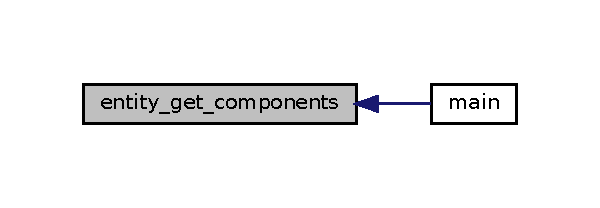
\includegraphics[width=288pt]{examples_2velocity_2include_2des_8h_a67e67b5444435172378a5e24701a02e7_icgraph}
\end{center}
\end{figure}
\mbox{\Hypertarget{examples_2velocity_2include_2des_8h_a44b8855c1b56396b8faedcd389fe4546}\label{examples_2velocity_2include_2des_8h_a44b8855c1b56396b8faedcd389fe4546}} 
\index{examples/velocity/include/des.\+h@{examples/velocity/include/des.\+h}!entity\+\_\+pool\+\_\+create@{entity\+\_\+pool\+\_\+create}}
\index{entity\+\_\+pool\+\_\+create@{entity\+\_\+pool\+\_\+create}!examples/velocity/include/des.\+h@{examples/velocity/include/des.\+h}}
\subsubsection{\texorpdfstring{entity\+\_\+pool\+\_\+create()}{entity\_pool\_create()}}
{\footnotesize\ttfamily \mbox{\hyperlink{struct_entity_pool}{Entity\+Pool}}$\ast$ entity\+\_\+pool\+\_\+create (\begin{DoxyParamCaption}\item[{int}]{size }\end{DoxyParamCaption})}



Create \mbox{\hyperlink{struct_entity_pool}{Entity\+Pool}} and malloc it\textquotesingle{}s component with the size provided, returns N\+U\+LL if insufficient R\+AM. 


\begin{DoxyParams}{Parameters}
{\em size} & \\
\hline
\end{DoxyParams}
\begin{DoxyReturn}{Returns}
Entity\+Pool$\ast$ 
\end{DoxyReturn}
Here is the caller graph for this function\+:\nopagebreak
\begin{figure}[H]
\begin{center}
\leavevmode
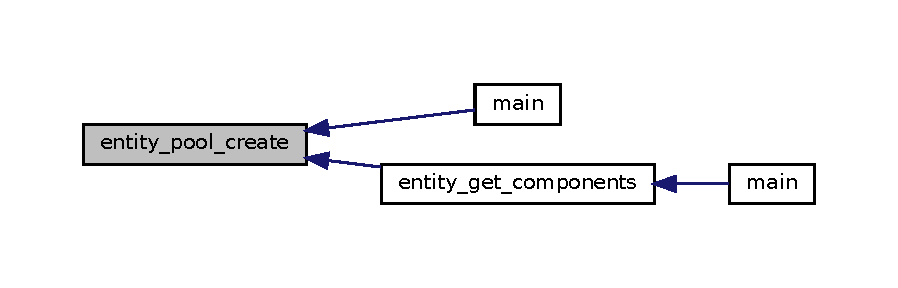
\includegraphics[width=350pt]{examples_2velocity_2include_2des_8h_a44b8855c1b56396b8faedcd389fe4546_icgraph}
\end{center}
\end{figure}
\mbox{\Hypertarget{examples_2velocity_2include_2des_8h_a3e377867fe9b332352eb47cdf9dc1a4c}\label{examples_2velocity_2include_2des_8h_a3e377867fe9b332352eb47cdf9dc1a4c}} 
\index{examples/velocity/include/des.\+h@{examples/velocity/include/des.\+h}!entity\+\_\+pool\+\_\+destroy@{entity\+\_\+pool\+\_\+destroy}}
\index{entity\+\_\+pool\+\_\+destroy@{entity\+\_\+pool\+\_\+destroy}!examples/velocity/include/des.\+h@{examples/velocity/include/des.\+h}}
\subsubsection{\texorpdfstring{entity\+\_\+pool\+\_\+destroy()}{entity\_pool\_destroy()}}
{\footnotesize\ttfamily void entity\+\_\+pool\+\_\+destroy (\begin{DoxyParamCaption}\item[{\mbox{\hyperlink{struct_entity_pool}{Entity\+Pool}} $\ast$}]{entity\+\_\+pool }\end{DoxyParamCaption})}



Free all memory allocated for the \mbox{\hyperlink{struct_entity_pool}{Entity\+Pool}}. 


\begin{DoxyParams}{Parameters}
{\em entity\+\_\+pool} & \\
\hline
\end{DoxyParams}
Here is the caller graph for this function\+:\nopagebreak
\begin{figure}[H]
\begin{center}
\leavevmode
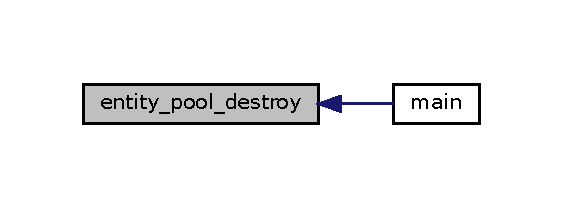
\includegraphics[width=270pt]{examples_2velocity_2include_2des_8h_a3e377867fe9b332352eb47cdf9dc1a4c_icgraph}
\end{center}
\end{figure}
\mbox{\Hypertarget{examples_2velocity_2include_2des_8h_a3955b16f45429c7ea74f275dac36493d}\label{examples_2velocity_2include_2des_8h_a3955b16f45429c7ea74f275dac36493d}} 
\index{examples/velocity/include/des.\+h@{examples/velocity/include/des.\+h}!entity\+\_\+pool\+\_\+find\+\_\+empty\+\_\+row@{entity\+\_\+pool\+\_\+find\+\_\+empty\+\_\+row}}
\index{entity\+\_\+pool\+\_\+find\+\_\+empty\+\_\+row@{entity\+\_\+pool\+\_\+find\+\_\+empty\+\_\+row}!examples/velocity/include/des.\+h@{examples/velocity/include/des.\+h}}
\subsubsection{\texorpdfstring{entity\+\_\+pool\+\_\+find\+\_\+empty\+\_\+row()}{entity\_pool\_find\_empty\_row()}}
{\footnotesize\ttfamily int entity\+\_\+pool\+\_\+find\+\_\+empty\+\_\+row (\begin{DoxyParamCaption}\item[{\mbox{\hyperlink{struct_entity_pool}{Entity\+Pool}} $\ast$}]{entity\+\_\+pool }\end{DoxyParamCaption})}



Find the index first empty row in the provided \mbox{\hyperlink{struct_entity_pool}{Entity\+Pool}}. 


\begin{DoxyParams}{Parameters}
{\em entity\+\_\+pool} & \\
\hline
\end{DoxyParams}
\begin{DoxyReturn}{Returns}
int 
\end{DoxyReturn}
\mbox{\Hypertarget{examples_2velocity_2include_2des_8h_a7fa6d71c51a14d7607b66722a1f17427}\label{examples_2velocity_2include_2des_8h_a7fa6d71c51a14d7607b66722a1f17427}} 
\index{examples/velocity/include/des.\+h@{examples/velocity/include/des.\+h}!entity\+\_\+remove@{entity\+\_\+remove}}
\index{entity\+\_\+remove@{entity\+\_\+remove}!examples/velocity/include/des.\+h@{examples/velocity/include/des.\+h}}
\subsubsection{\texorpdfstring{entity\+\_\+remove()}{entity\_remove()}}
{\footnotesize\ttfamily void entity\+\_\+remove (\begin{DoxyParamCaption}\item[{\mbox{\hyperlink{struct_entity_pool}{Entity\+Pool}} $\ast$}]{entity\+\_\+pool,  }\item[{int}]{guid }\end{DoxyParamCaption})}



Remove all data on the entity in the provided \mbox{\hyperlink{struct_entity_pool}{Entity\+Pool}}. 


\begin{DoxyParams}{Parameters}
{\em entity\+\_\+pool} & \\
\hline
{\em guid} & \\
\hline
\end{DoxyParams}

\hypertarget{include_2des_8h}{}\section{/home/drvanon/\+Documents/scripts/\+D\+E\+S/include/des.h File Reference}
\label{include_2des_8h}\index{/home/drvanon/\+Documents/scripts/\+D\+E\+S/include/des.\+h@{/home/drvanon/\+Documents/scripts/\+D\+E\+S/include/des.\+h}}
{\ttfamily \#include \char`\"{}entity.\+h\char`\"{}}\newline
{\ttfamily \#include \char`\"{}component.\+h\char`\"{}}\newline
{\ttfamily \#include \char`\"{}assemblage.\+h\char`\"{}}\newline
Include dependency graph for des.\+h\+:\nopagebreak
\begin{figure}[H]
\begin{center}
\leavevmode
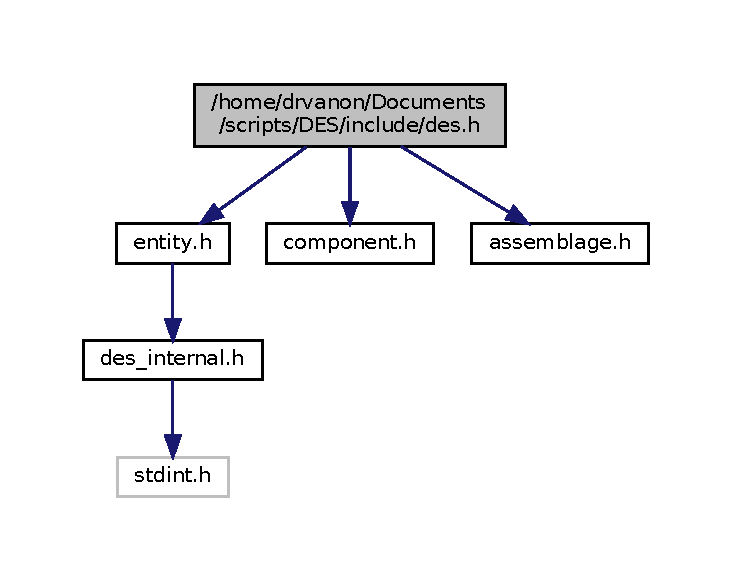
\includegraphics[width=350pt]{include_2des_8h__incl}
\end{center}
\end{figure}
This graph shows which files directly or indirectly include this file\+:\nopagebreak
\begin{figure}[H]
\begin{center}
\leavevmode
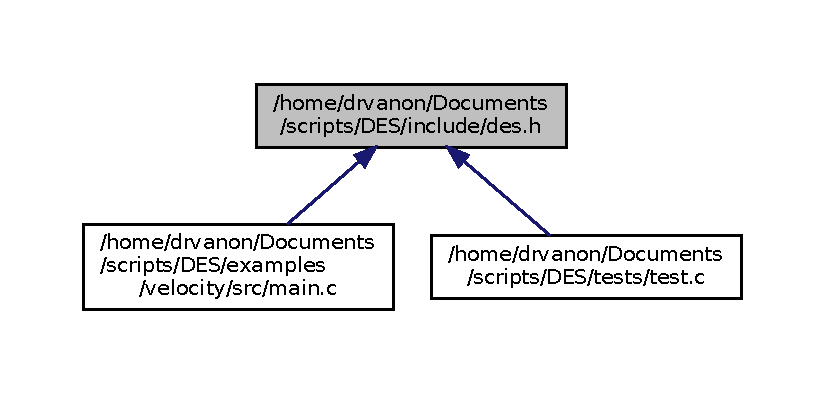
\includegraphics[width=350pt]{include_2des_8h__dep__incl}
\end{center}
\end{figure}

\hypertarget{examples_2velocity_2include_2des__internal_8h}{}\section{/home/drvanon/\+Documents/scripts/\+D\+E\+S/examples/velocity/include/des\+\_\+internal.h File Reference}
\label{examples_2velocity_2include_2des__internal_8h}\index{/home/drvanon/\+Documents/scripts/\+D\+E\+S/examples/velocity/include/des\+\_\+internal.\+h@{/home/drvanon/\+Documents/scripts/\+D\+E\+S/examples/velocity/include/des\+\_\+internal.\+h}}
{\ttfamily \#include $<$stdint.\+h$>$}\newline
Include dependency graph for des\+\_\+internal.\+h\+:\nopagebreak
\begin{figure}[H]
\begin{center}
\leavevmode
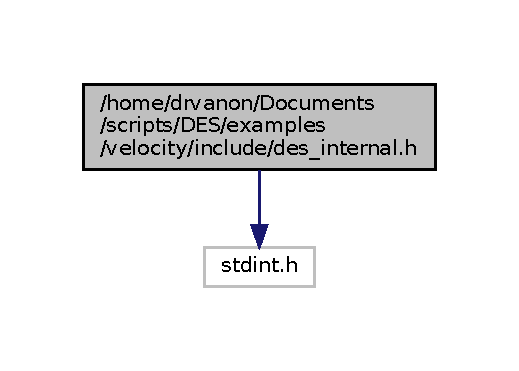
\includegraphics[width=249pt]{examples_2velocity_2include_2des__internal_8h__incl}
\end{center}
\end{figure}
This graph shows which files directly or indirectly include this file\+:\nopagebreak
\begin{figure}[H]
\begin{center}
\leavevmode
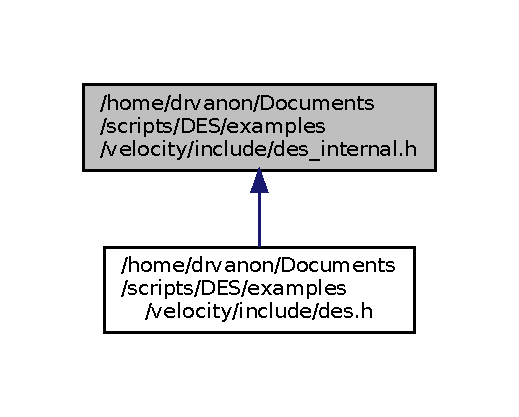
\includegraphics[width=249pt]{examples_2velocity_2include_2des__internal_8h__dep__incl}
\end{center}
\end{figure}
\subsection*{Typedefs}
\begin{DoxyCompactItemize}
\item 
typedef uint8\+\_\+t \mbox{\hyperlink{examples_2velocity_2include_2des__internal_8h_a0a6c75fe16fd8f3a830e24da31d2194a}{i8}}
\item 
typedef uint16\+\_\+t \mbox{\hyperlink{examples_2velocity_2include_2des__internal_8h_a9b039d6a413a3c72b6e95929d5ec8731}{i16}}
\item 
typedef uint32\+\_\+t \mbox{\hyperlink{examples_2velocity_2include_2des__internal_8h_ab29dd86df14bc64fb2ed55c3b3445c72}{i32}}
\item 
typedef uint64\+\_\+t \mbox{\hyperlink{examples_2velocity_2include_2des__internal_8h_a906bea3c89bdda9386c6d00bb3bacd72}{i64}}
\item 
typedef uint8\+\_\+t \mbox{\hyperlink{examples_2velocity_2include_2des__internal_8h_a92c50087ca0e64fa93fc59402c55f8ca}{u8}}
\item 
typedef uint16\+\_\+t \mbox{\hyperlink{examples_2velocity_2include_2des__internal_8h_ace9d960e74685e2cd84b36132dbbf8aa}{u16}}
\item 
typedef uint32\+\_\+t \mbox{\hyperlink{examples_2velocity_2include_2des__internal_8h_afaa62991928fb9fb18ff0db62a040aba}{u32}}
\item 
typedef uint64\+\_\+t \mbox{\hyperlink{examples_2velocity_2include_2des__internal_8h_a3f7e2bcbb0b4c338f3c4f6c937cd4234}{u64}}
\end{DoxyCompactItemize}


\subsection{Typedef Documentation}
\mbox{\Hypertarget{examples_2velocity_2include_2des__internal_8h_a9b039d6a413a3c72b6e95929d5ec8731}\label{examples_2velocity_2include_2des__internal_8h_a9b039d6a413a3c72b6e95929d5ec8731}} 
\index{examples/velocity/include/des\+\_\+internal.\+h@{examples/velocity/include/des\+\_\+internal.\+h}!i16@{i16}}
\index{i16@{i16}!examples/velocity/include/des\+\_\+internal.\+h@{examples/velocity/include/des\+\_\+internal.\+h}}
\subsubsection{\texorpdfstring{i16}{i16}}
{\footnotesize\ttfamily typedef uint16\+\_\+t \mbox{\hyperlink{examples_2velocity_2include_2des__internal_8h_a9b039d6a413a3c72b6e95929d5ec8731}{i16}}}

\mbox{\Hypertarget{examples_2velocity_2include_2des__internal_8h_ab29dd86df14bc64fb2ed55c3b3445c72}\label{examples_2velocity_2include_2des__internal_8h_ab29dd86df14bc64fb2ed55c3b3445c72}} 
\index{examples/velocity/include/des\+\_\+internal.\+h@{examples/velocity/include/des\+\_\+internal.\+h}!i32@{i32}}
\index{i32@{i32}!examples/velocity/include/des\+\_\+internal.\+h@{examples/velocity/include/des\+\_\+internal.\+h}}
\subsubsection{\texorpdfstring{i32}{i32}}
{\footnotesize\ttfamily typedef uint32\+\_\+t \mbox{\hyperlink{examples_2velocity_2include_2des__internal_8h_ab29dd86df14bc64fb2ed55c3b3445c72}{i32}}}

\mbox{\Hypertarget{examples_2velocity_2include_2des__internal_8h_a906bea3c89bdda9386c6d00bb3bacd72}\label{examples_2velocity_2include_2des__internal_8h_a906bea3c89bdda9386c6d00bb3bacd72}} 
\index{examples/velocity/include/des\+\_\+internal.\+h@{examples/velocity/include/des\+\_\+internal.\+h}!i64@{i64}}
\index{i64@{i64}!examples/velocity/include/des\+\_\+internal.\+h@{examples/velocity/include/des\+\_\+internal.\+h}}
\subsubsection{\texorpdfstring{i64}{i64}}
{\footnotesize\ttfamily typedef uint64\+\_\+t \mbox{\hyperlink{examples_2velocity_2include_2des__internal_8h_a906bea3c89bdda9386c6d00bb3bacd72}{i64}}}

\mbox{\Hypertarget{examples_2velocity_2include_2des__internal_8h_a0a6c75fe16fd8f3a830e24da31d2194a}\label{examples_2velocity_2include_2des__internal_8h_a0a6c75fe16fd8f3a830e24da31d2194a}} 
\index{examples/velocity/include/des\+\_\+internal.\+h@{examples/velocity/include/des\+\_\+internal.\+h}!i8@{i8}}
\index{i8@{i8}!examples/velocity/include/des\+\_\+internal.\+h@{examples/velocity/include/des\+\_\+internal.\+h}}
\subsubsection{\texorpdfstring{i8}{i8}}
{\footnotesize\ttfamily typedef uint8\+\_\+t \mbox{\hyperlink{examples_2velocity_2include_2des__internal_8h_a0a6c75fe16fd8f3a830e24da31d2194a}{i8}}}

\mbox{\Hypertarget{examples_2velocity_2include_2des__internal_8h_ace9d960e74685e2cd84b36132dbbf8aa}\label{examples_2velocity_2include_2des__internal_8h_ace9d960e74685e2cd84b36132dbbf8aa}} 
\index{examples/velocity/include/des\+\_\+internal.\+h@{examples/velocity/include/des\+\_\+internal.\+h}!u16@{u16}}
\index{u16@{u16}!examples/velocity/include/des\+\_\+internal.\+h@{examples/velocity/include/des\+\_\+internal.\+h}}
\subsubsection{\texorpdfstring{u16}{u16}}
{\footnotesize\ttfamily typedef uint16\+\_\+t \mbox{\hyperlink{examples_2velocity_2include_2des__internal_8h_ace9d960e74685e2cd84b36132dbbf8aa}{u16}}}

\mbox{\Hypertarget{examples_2velocity_2include_2des__internal_8h_afaa62991928fb9fb18ff0db62a040aba}\label{examples_2velocity_2include_2des__internal_8h_afaa62991928fb9fb18ff0db62a040aba}} 
\index{examples/velocity/include/des\+\_\+internal.\+h@{examples/velocity/include/des\+\_\+internal.\+h}!u32@{u32}}
\index{u32@{u32}!examples/velocity/include/des\+\_\+internal.\+h@{examples/velocity/include/des\+\_\+internal.\+h}}
\subsubsection{\texorpdfstring{u32}{u32}}
{\footnotesize\ttfamily typedef uint32\+\_\+t \mbox{\hyperlink{examples_2velocity_2include_2des__internal_8h_afaa62991928fb9fb18ff0db62a040aba}{u32}}}

\mbox{\Hypertarget{examples_2velocity_2include_2des__internal_8h_a3f7e2bcbb0b4c338f3c4f6c937cd4234}\label{examples_2velocity_2include_2des__internal_8h_a3f7e2bcbb0b4c338f3c4f6c937cd4234}} 
\index{examples/velocity/include/des\+\_\+internal.\+h@{examples/velocity/include/des\+\_\+internal.\+h}!u64@{u64}}
\index{u64@{u64}!examples/velocity/include/des\+\_\+internal.\+h@{examples/velocity/include/des\+\_\+internal.\+h}}
\subsubsection{\texorpdfstring{u64}{u64}}
{\footnotesize\ttfamily typedef uint64\+\_\+t \mbox{\hyperlink{examples_2velocity_2include_2des__internal_8h_a3f7e2bcbb0b4c338f3c4f6c937cd4234}{u64}}}

\mbox{\Hypertarget{examples_2velocity_2include_2des__internal_8h_a92c50087ca0e64fa93fc59402c55f8ca}\label{examples_2velocity_2include_2des__internal_8h_a92c50087ca0e64fa93fc59402c55f8ca}} 
\index{examples/velocity/include/des\+\_\+internal.\+h@{examples/velocity/include/des\+\_\+internal.\+h}!u8@{u8}}
\index{u8@{u8}!examples/velocity/include/des\+\_\+internal.\+h@{examples/velocity/include/des\+\_\+internal.\+h}}
\subsubsection{\texorpdfstring{u8}{u8}}
{\footnotesize\ttfamily typedef uint8\+\_\+t \mbox{\hyperlink{examples_2velocity_2include_2des__internal_8h_a92c50087ca0e64fa93fc59402c55f8ca}{u8}}}


\hypertarget{include_2des__internal_8h}{}\section{/home/drvanon/\+Documents/scripts/\+D\+E\+S/include/des\+\_\+internal.h File Reference}
\label{include_2des__internal_8h}\index{/home/drvanon/\+Documents/scripts/\+D\+E\+S/include/des\+\_\+internal.\+h@{/home/drvanon/\+Documents/scripts/\+D\+E\+S/include/des\+\_\+internal.\+h}}
{\ttfamily \#include $<$stdint.\+h$>$}\newline
Include dependency graph for des\+\_\+internal.\+h\+:\nopagebreak
\begin{figure}[H]
\begin{center}
\leavevmode
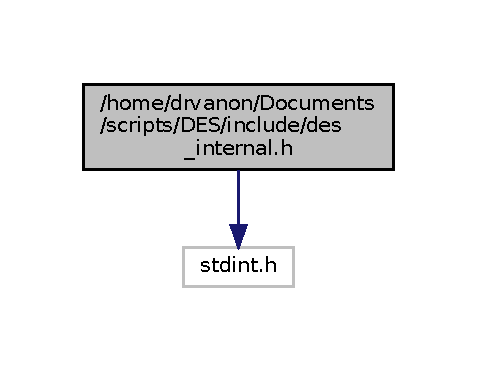
\includegraphics[width=229pt]{include_2des__internal_8h__incl}
\end{center}
\end{figure}
This graph shows which files directly or indirectly include this file\+:\nopagebreak
\begin{figure}[H]
\begin{center}
\leavevmode
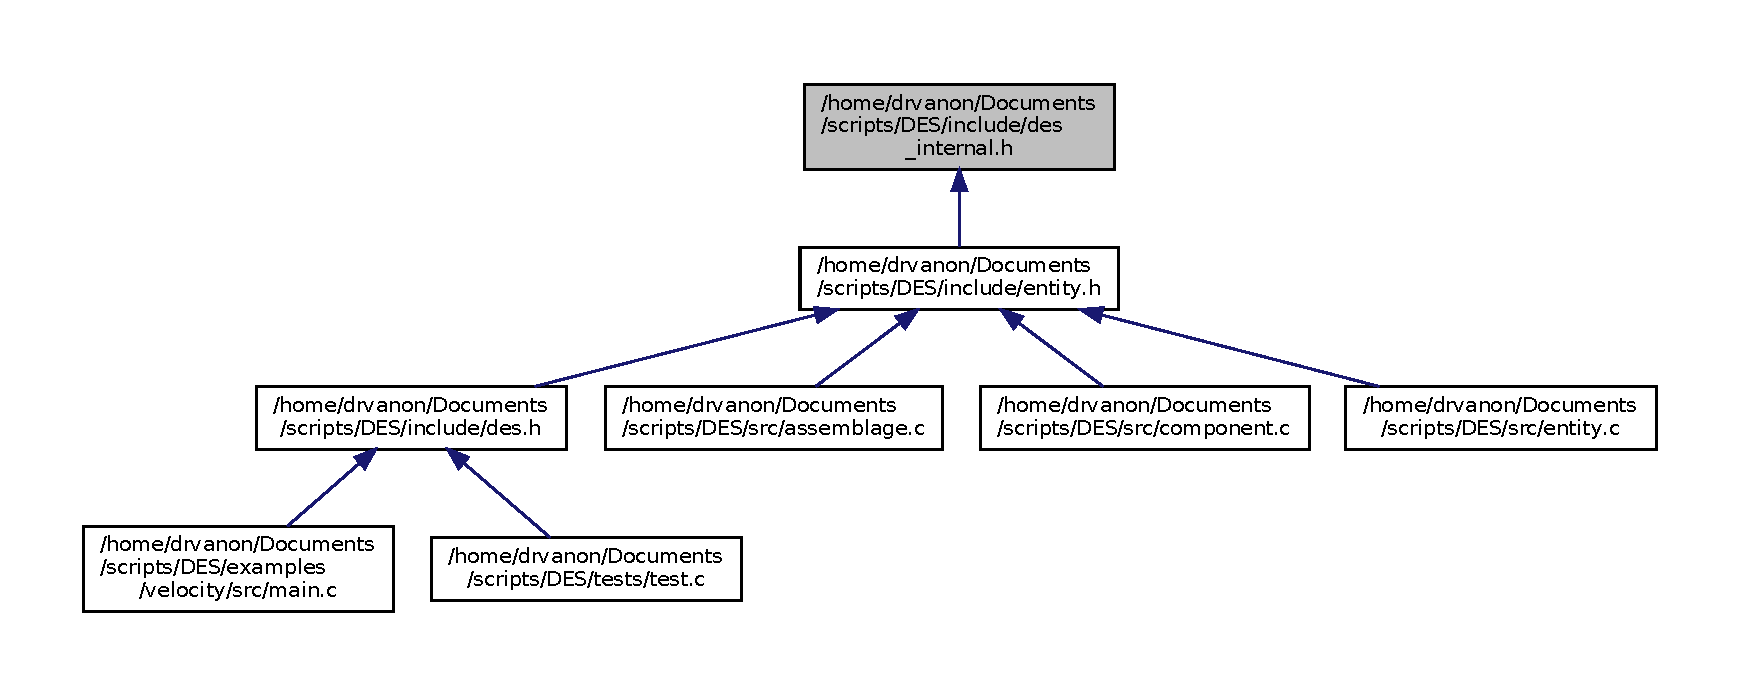
\includegraphics[width=350pt]{include_2des__internal_8h__dep__incl}
\end{center}
\end{figure}
\subsection*{Typedefs}
\begin{DoxyCompactItemize}
\item 
typedef uint8\+\_\+t \mbox{\hyperlink{include_2des__internal_8h_a0a6c75fe16fd8f3a830e24da31d2194a}{i8}}
\item 
typedef uint16\+\_\+t \mbox{\hyperlink{include_2des__internal_8h_a9b039d6a413a3c72b6e95929d5ec8731}{i16}}
\item 
typedef uint32\+\_\+t \mbox{\hyperlink{include_2des__internal_8h_ab29dd86df14bc64fb2ed55c3b3445c72}{i32}}
\item 
typedef uint64\+\_\+t \mbox{\hyperlink{include_2des__internal_8h_a906bea3c89bdda9386c6d00bb3bacd72}{i64}}
\item 
typedef uint8\+\_\+t \mbox{\hyperlink{include_2des__internal_8h_a92c50087ca0e64fa93fc59402c55f8ca}{u8}}
\item 
typedef uint16\+\_\+t \mbox{\hyperlink{include_2des__internal_8h_ace9d960e74685e2cd84b36132dbbf8aa}{u16}}
\item 
typedef uint32\+\_\+t \mbox{\hyperlink{include_2des__internal_8h_afaa62991928fb9fb18ff0db62a040aba}{u32}}
\item 
typedef uint64\+\_\+t \mbox{\hyperlink{include_2des__internal_8h_a3f7e2bcbb0b4c338f3c4f6c937cd4234}{u64}}
\end{DoxyCompactItemize}


\subsection{Typedef Documentation}
\mbox{\Hypertarget{include_2des__internal_8h_a9b039d6a413a3c72b6e95929d5ec8731}\label{include_2des__internal_8h_a9b039d6a413a3c72b6e95929d5ec8731}} 
\index{include/des\+\_\+internal.\+h@{include/des\+\_\+internal.\+h}!i16@{i16}}
\index{i16@{i16}!include/des\+\_\+internal.\+h@{include/des\+\_\+internal.\+h}}
\subsubsection{\texorpdfstring{i16}{i16}}
{\footnotesize\ttfamily typedef uint16\+\_\+t \mbox{\hyperlink{examples_2velocity_2include_2des__internal_8h_a9b039d6a413a3c72b6e95929d5ec8731}{i16}}}

\mbox{\Hypertarget{include_2des__internal_8h_ab29dd86df14bc64fb2ed55c3b3445c72}\label{include_2des__internal_8h_ab29dd86df14bc64fb2ed55c3b3445c72}} 
\index{include/des\+\_\+internal.\+h@{include/des\+\_\+internal.\+h}!i32@{i32}}
\index{i32@{i32}!include/des\+\_\+internal.\+h@{include/des\+\_\+internal.\+h}}
\subsubsection{\texorpdfstring{i32}{i32}}
{\footnotesize\ttfamily typedef uint32\+\_\+t \mbox{\hyperlink{examples_2velocity_2include_2des__internal_8h_ab29dd86df14bc64fb2ed55c3b3445c72}{i32}}}

\mbox{\Hypertarget{include_2des__internal_8h_a906bea3c89bdda9386c6d00bb3bacd72}\label{include_2des__internal_8h_a906bea3c89bdda9386c6d00bb3bacd72}} 
\index{include/des\+\_\+internal.\+h@{include/des\+\_\+internal.\+h}!i64@{i64}}
\index{i64@{i64}!include/des\+\_\+internal.\+h@{include/des\+\_\+internal.\+h}}
\subsubsection{\texorpdfstring{i64}{i64}}
{\footnotesize\ttfamily typedef uint64\+\_\+t \mbox{\hyperlink{examples_2velocity_2include_2des__internal_8h_a906bea3c89bdda9386c6d00bb3bacd72}{i64}}}

\mbox{\Hypertarget{include_2des__internal_8h_a0a6c75fe16fd8f3a830e24da31d2194a}\label{include_2des__internal_8h_a0a6c75fe16fd8f3a830e24da31d2194a}} 
\index{include/des\+\_\+internal.\+h@{include/des\+\_\+internal.\+h}!i8@{i8}}
\index{i8@{i8}!include/des\+\_\+internal.\+h@{include/des\+\_\+internal.\+h}}
\subsubsection{\texorpdfstring{i8}{i8}}
{\footnotesize\ttfamily typedef uint8\+\_\+t \mbox{\hyperlink{examples_2velocity_2include_2des__internal_8h_a0a6c75fe16fd8f3a830e24da31d2194a}{i8}}}

\mbox{\Hypertarget{include_2des__internal_8h_ace9d960e74685e2cd84b36132dbbf8aa}\label{include_2des__internal_8h_ace9d960e74685e2cd84b36132dbbf8aa}} 
\index{include/des\+\_\+internal.\+h@{include/des\+\_\+internal.\+h}!u16@{u16}}
\index{u16@{u16}!include/des\+\_\+internal.\+h@{include/des\+\_\+internal.\+h}}
\subsubsection{\texorpdfstring{u16}{u16}}
{\footnotesize\ttfamily typedef uint16\+\_\+t \mbox{\hyperlink{examples_2velocity_2include_2des__internal_8h_ace9d960e74685e2cd84b36132dbbf8aa}{u16}}}

\mbox{\Hypertarget{include_2des__internal_8h_afaa62991928fb9fb18ff0db62a040aba}\label{include_2des__internal_8h_afaa62991928fb9fb18ff0db62a040aba}} 
\index{include/des\+\_\+internal.\+h@{include/des\+\_\+internal.\+h}!u32@{u32}}
\index{u32@{u32}!include/des\+\_\+internal.\+h@{include/des\+\_\+internal.\+h}}
\subsubsection{\texorpdfstring{u32}{u32}}
{\footnotesize\ttfamily typedef uint32\+\_\+t \mbox{\hyperlink{examples_2velocity_2include_2des__internal_8h_afaa62991928fb9fb18ff0db62a040aba}{u32}}}

\mbox{\Hypertarget{include_2des__internal_8h_a3f7e2bcbb0b4c338f3c4f6c937cd4234}\label{include_2des__internal_8h_a3f7e2bcbb0b4c338f3c4f6c937cd4234}} 
\index{include/des\+\_\+internal.\+h@{include/des\+\_\+internal.\+h}!u64@{u64}}
\index{u64@{u64}!include/des\+\_\+internal.\+h@{include/des\+\_\+internal.\+h}}
\subsubsection{\texorpdfstring{u64}{u64}}
{\footnotesize\ttfamily typedef uint64\+\_\+t \mbox{\hyperlink{examples_2velocity_2include_2des__internal_8h_a3f7e2bcbb0b4c338f3c4f6c937cd4234}{u64}}}

\mbox{\Hypertarget{include_2des__internal_8h_a92c50087ca0e64fa93fc59402c55f8ca}\label{include_2des__internal_8h_a92c50087ca0e64fa93fc59402c55f8ca}} 
\index{include/des\+\_\+internal.\+h@{include/des\+\_\+internal.\+h}!u8@{u8}}
\index{u8@{u8}!include/des\+\_\+internal.\+h@{include/des\+\_\+internal.\+h}}
\subsubsection{\texorpdfstring{u8}{u8}}
{\footnotesize\ttfamily typedef uint8\+\_\+t \mbox{\hyperlink{examples_2velocity_2include_2des__internal_8h_a92c50087ca0e64fa93fc59402c55f8ca}{u8}}}


\hypertarget{examples_2velocity_2obj_2src_2main_8o_8d}{}\section{/home/drvanon/\+Documents/scripts/\+D\+E\+S/examples/velocity/obj/src/main.o.\+d File Reference}
\label{examples_2velocity_2obj_2src_2main_8o_8d}\index{/home/drvanon/\+Documents/scripts/\+D\+E\+S/examples/velocity/obj/src/main.\+o.\+d@{/home/drvanon/\+Documents/scripts/\+D\+E\+S/examples/velocity/obj/src/main.\+o.\+d}}

\hypertarget{obj_2src_2main_8o_8d}{}\section{/home/drvanon/\+Documents/scripts/\+D\+E\+S/obj/src/main.o.\+d File Reference}
\label{obj_2src_2main_8o_8d}\index{/home/drvanon/\+Documents/scripts/\+D\+E\+S/obj/src/main.\+o.\+d@{/home/drvanon/\+Documents/scripts/\+D\+E\+S/obj/src/main.\+o.\+d}}

\hypertarget{examples_2velocity_2obj_2src_2systems_2system__velocity_8o_8d}{}\section{/home/drvanon/\+Documents/scripts/\+D\+E\+S/examples/velocity/obj/src/systems/system\+\_\+velocity.o.\+d File Reference}
\label{examples_2velocity_2obj_2src_2systems_2system__velocity_8o_8d}\index{/home/drvanon/\+Documents/scripts/\+D\+E\+S/examples/velocity/obj/src/systems/system\+\_\+velocity.\+o.\+d@{/home/drvanon/\+Documents/scripts/\+D\+E\+S/examples/velocity/obj/src/systems/system\+\_\+velocity.\+o.\+d}}

\hypertarget{obj_2src_2system_2system__velocity_8o_8d}{}\section{/home/drvanon/\+Documents/scripts/\+D\+E\+S/obj/src/system/system\+\_\+velocity.o.\+d File Reference}
\label{obj_2src_2system_2system__velocity_8o_8d}\index{/home/drvanon/\+Documents/scripts/\+D\+E\+S/obj/src/system/system\+\_\+velocity.\+o.\+d@{/home/drvanon/\+Documents/scripts/\+D\+E\+S/obj/src/system/system\+\_\+velocity.\+o.\+d}}

\hypertarget{obj_2src_2systems_2system__velocity_8o_8d}{}\section{/home/drvanon/\+Documents/scripts/\+D\+E\+S/obj/src/systems/system\+\_\+velocity.o.\+d File Reference}
\label{obj_2src_2systems_2system__velocity_8o_8d}\index{/home/drvanon/\+Documents/scripts/\+D\+E\+S/obj/src/systems/system\+\_\+velocity.\+o.\+d@{/home/drvanon/\+Documents/scripts/\+D\+E\+S/obj/src/systems/system\+\_\+velocity.\+o.\+d}}

\hypertarget{components_8h}{}\section{components/components.h File Reference}
\label{components_8h}\index{components/components.\+h@{components/components.\+h}}
This graph shows which files directly or indirectly include this file\+:\nopagebreak
\begin{figure}[H]
\begin{center}
\leavevmode
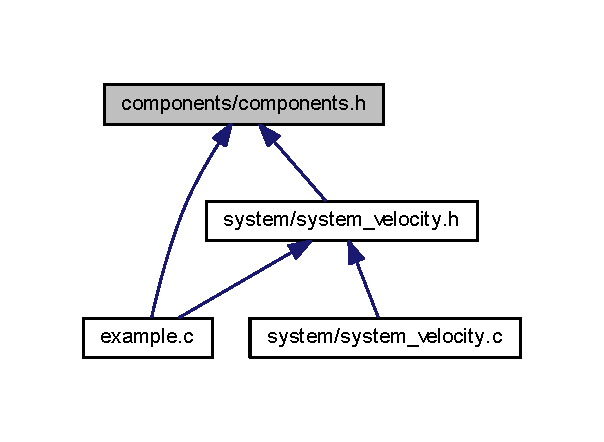
\includegraphics[width=290pt]{components_8h__dep__incl}
\end{center}
\end{figure}
\subsection*{Data Structures}
\begin{DoxyCompactItemize}
\item 
struct \mbox{\hyperlink{struct_position_component_pool}{Position\+Component\+Pool}}
\begin{DoxyCompactList}\small\item\em Component for the position of the entity. \end{DoxyCompactList}\item 
struct \mbox{\hyperlink{struct_velocity_component_pool}{Velocity\+Component\+Pool}}
\begin{DoxyCompactList}\small\item\em Component with the velocity data. This gets added to the position by a system. \end{DoxyCompactList}\end{DoxyCompactItemize}
\subsection*{Typedefs}
\begin{DoxyCompactItemize}
\item 
typedef struct \mbox{\hyperlink{struct_position_component_pool}{Position\+Component\+Pool}} \mbox{\hyperlink{components_8h_a08b5b44ed4269e8c3ff11ffdbfae8791}{Position\+Component\+Pool}}
\begin{DoxyCompactList}\small\item\em Component for the position of the entity. \end{DoxyCompactList}\item 
typedef struct \mbox{\hyperlink{struct_velocity_component_pool}{Velocity\+Component\+Pool}} \mbox{\hyperlink{components_8h_a5005a04501037e679a563e6fdd31f464}{Velocity\+Component\+Pool}}
\begin{DoxyCompactList}\small\item\em Component with the velocity data. This gets added to the position by a system. \end{DoxyCompactList}\end{DoxyCompactItemize}


\subsection{Typedef Documentation}
\mbox{\Hypertarget{components_8h_a08b5b44ed4269e8c3ff11ffdbfae8791}\label{components_8h_a08b5b44ed4269e8c3ff11ffdbfae8791}} 
\index{components.\+h@{components.\+h}!Position\+Component\+Pool@{Position\+Component\+Pool}}
\index{Position\+Component\+Pool@{Position\+Component\+Pool}!components.\+h@{components.\+h}}
\subsubsection{\texorpdfstring{Position\+Component\+Pool}{PositionComponentPool}}
{\footnotesize\ttfamily typedef struct \mbox{\hyperlink{struct_position_component_pool}{Position\+Component\+Pool}}  \mbox{\hyperlink{struct_position_component_pool}{Position\+Component\+Pool}}}



Component for the position of the entity. 

\mbox{\Hypertarget{components_8h_a5005a04501037e679a563e6fdd31f464}\label{components_8h_a5005a04501037e679a563e6fdd31f464}} 
\index{components.\+h@{components.\+h}!Velocity\+Component\+Pool@{Velocity\+Component\+Pool}}
\index{Velocity\+Component\+Pool@{Velocity\+Component\+Pool}!components.\+h@{components.\+h}}
\subsubsection{\texorpdfstring{Velocity\+Component\+Pool}{VelocityComponentPool}}
{\footnotesize\ttfamily typedef struct \mbox{\hyperlink{struct_velocity_component_pool}{Velocity\+Component\+Pool}}  \mbox{\hyperlink{struct_velocity_component_pool}{Velocity\+Component\+Pool}}}



Component with the velocity data. This gets added to the position by a system. 


\hypertarget{main_8c}{}\section{/home/drvanon/\+Documents/scripts/\+D\+E\+S/examples/velocity/src/main.c File Reference}
\label{main_8c}\index{/home/drvanon/\+Documents/scripts/\+D\+E\+S/examples/velocity/src/main.\+c@{/home/drvanon/\+Documents/scripts/\+D\+E\+S/examples/velocity/src/main.\+c}}
{\ttfamily \#include $<$stdio.\+h$>$}\newline
{\ttfamily \#include $<$stdlib.\+h$>$}\newline
{\ttfamily \#include $<$time.\+h$>$}\newline
{\ttfamily \#include \char`\"{}des.\+h\char`\"{}}\newline
{\ttfamily \#include \char`\"{}components.\+h\char`\"{}}\newline
{\ttfamily \#include \char`\"{}system\+\_\+velocity.\+h\char`\"{}}\newline
Include dependency graph for main.\+c\+:\nopagebreak
\begin{figure}[H]
\begin{center}
\leavevmode
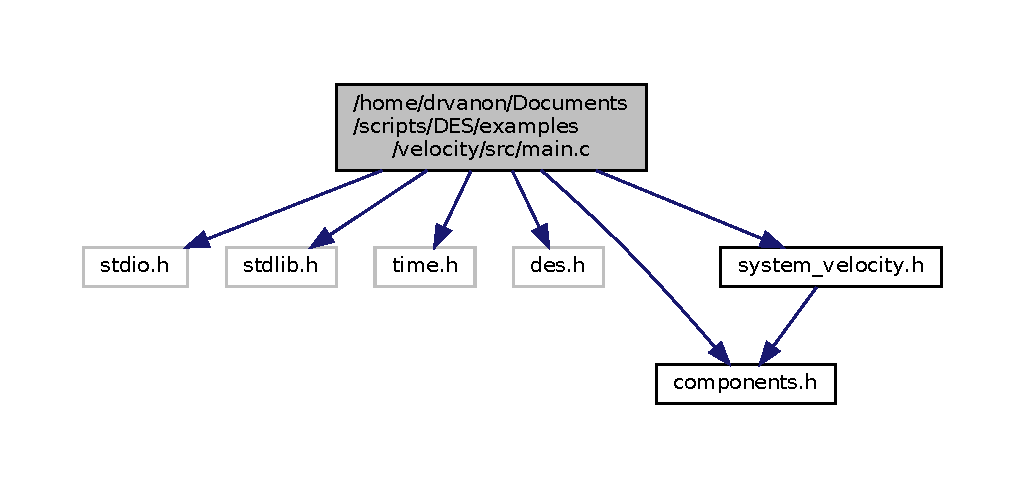
\includegraphics[width=350pt]{main_8c__incl}
\end{center}
\end{figure}
\subsection*{Macros}
\begin{DoxyCompactItemize}
\item 
\#define \mbox{\hyperlink{main_8c_a9d1db42a5fe2d7bf9f4958db88a3029b}{P\+O\+O\+L\+S\+I\+ZE}}~2048
\end{DoxyCompactItemize}
\subsection*{Functions}
\begin{DoxyCompactItemize}
\item 
int \mbox{\hyperlink{main_8c_ae66f6b31b5ad750f1fe042a706a4e3d4}{main}} ()
\end{DoxyCompactItemize}


\subsection{Macro Definition Documentation}
\mbox{\Hypertarget{main_8c_a9d1db42a5fe2d7bf9f4958db88a3029b}\label{main_8c_a9d1db42a5fe2d7bf9f4958db88a3029b}} 
\index{main.\+c@{main.\+c}!P\+O\+O\+L\+S\+I\+ZE@{P\+O\+O\+L\+S\+I\+ZE}}
\index{P\+O\+O\+L\+S\+I\+ZE@{P\+O\+O\+L\+S\+I\+ZE}!main.\+c@{main.\+c}}
\subsubsection{\texorpdfstring{P\+O\+O\+L\+S\+I\+ZE}{POOLSIZE}}
{\footnotesize\ttfamily \#define P\+O\+O\+L\+S\+I\+ZE~2048}



\subsection{Function Documentation}
\mbox{\Hypertarget{main_8c_ae66f6b31b5ad750f1fe042a706a4e3d4}\label{main_8c_ae66f6b31b5ad750f1fe042a706a4e3d4}} 
\index{main.\+c@{main.\+c}!main@{main}}
\index{main@{main}!main.\+c@{main.\+c}}
\subsubsection{\texorpdfstring{main()}{main()}}
{\footnotesize\ttfamily int main (\begin{DoxyParamCaption}{ }\end{DoxyParamCaption})}

Here is the call graph for this function\+:\nopagebreak
\begin{figure}[H]
\begin{center}
\leavevmode
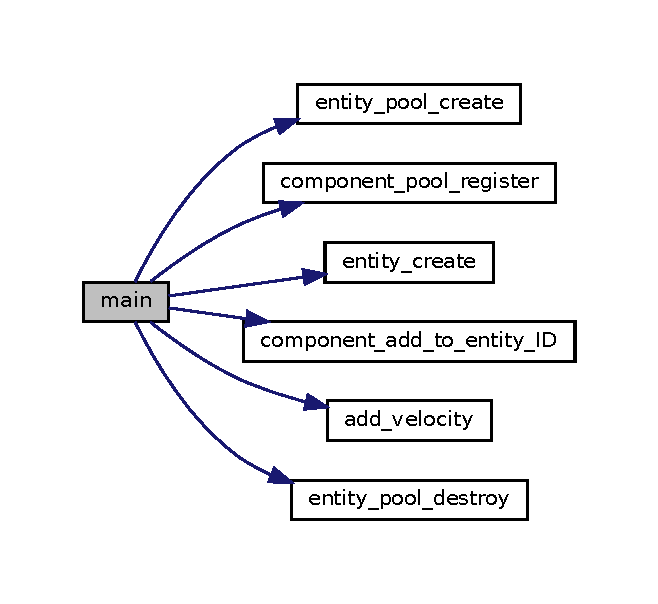
\includegraphics[width=316pt]{main_8c_ae66f6b31b5ad750f1fe042a706a4e3d4_cgraph}
\end{center}
\end{figure}

\hypertarget{system__velocity_8c}{}\section{/home/drvanon/\+Documents/scripts/\+D\+E\+S/examples/velocity/src/systems/system\+\_\+velocity.c File Reference}
\label{system__velocity_8c}\index{/home/drvanon/\+Documents/scripts/\+D\+E\+S/examples/velocity/src/systems/system\+\_\+velocity.\+c@{/home/drvanon/\+Documents/scripts/\+D\+E\+S/examples/velocity/src/systems/system\+\_\+velocity.\+c}}
{\ttfamily \#include \char`\"{}system\+\_\+velocity.\+h\char`\"{}}\newline
Include dependency graph for system\+\_\+velocity.\+c\+:\nopagebreak
\begin{figure}[H]
\begin{center}
\leavevmode
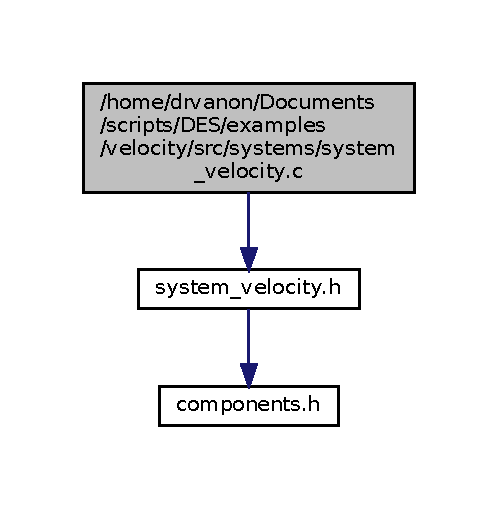
\includegraphics[width=239pt]{system__velocity_8c__incl}
\end{center}
\end{figure}
\subsection*{Functions}
\begin{DoxyCompactItemize}
\item 
void \mbox{\hyperlink{system__velocity_8c_a9b052269b4956842d12134a81e066d81}{add\+\_\+velocity}} (\mbox{\hyperlink{struct_position_component_pool}{Position\+Component\+Pool}} $\ast$position\+\_\+component\+\_\+pool, \mbox{\hyperlink{struct_velocity_component_pool}{Velocity\+Component\+Pool}} $\ast$velocity\+\_\+component\+\_\+pool)
\end{DoxyCompactItemize}


\subsection{Function Documentation}
\mbox{\Hypertarget{system__velocity_8c_a9b052269b4956842d12134a81e066d81}\label{system__velocity_8c_a9b052269b4956842d12134a81e066d81}} 
\index{system\+\_\+velocity.\+c@{system\+\_\+velocity.\+c}!add\+\_\+velocity@{add\+\_\+velocity}}
\index{add\+\_\+velocity@{add\+\_\+velocity}!system\+\_\+velocity.\+c@{system\+\_\+velocity.\+c}}
\subsubsection{\texorpdfstring{add\+\_\+velocity()}{add\_velocity()}}
{\footnotesize\ttfamily void add\+\_\+velocity (\begin{DoxyParamCaption}\item[{\mbox{\hyperlink{struct_position_component_pool}{Position\+Component\+Pool}} $\ast$}]{position\+\_\+component\+\_\+pool,  }\item[{\mbox{\hyperlink{struct_velocity_component_pool}{Velocity\+Component\+Pool}} $\ast$}]{velocity\+\_\+component\+\_\+pool }\end{DoxyParamCaption})}

Here is the caller graph for this function\+:\nopagebreak
\begin{figure}[H]
\begin{center}
\leavevmode
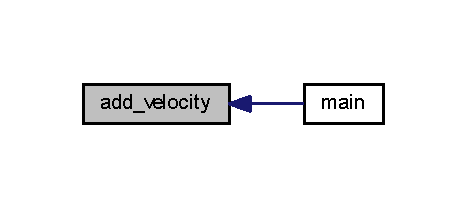
\includegraphics[width=236pt]{system__velocity_8c_a9b052269b4956842d12134a81e066d81_icgraph}
\end{center}
\end{figure}

\hypertarget{system__velocity_8h}{}\section{system/system\+\_\+velocity.h File Reference}
\label{system__velocity_8h}\index{system/system\+\_\+velocity.\+h@{system/system\+\_\+velocity.\+h}}
{\ttfamily \#include \char`\"{}components.\+h\char`\"{}}\newline
Include dependency graph for system\+\_\+velocity.\+h\+:\nopagebreak
\begin{figure}[H]
\begin{center}
\leavevmode
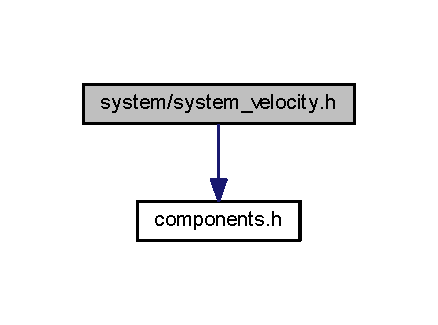
\includegraphics[width=210pt]{system__velocity_8h__incl}
\end{center}
\end{figure}
This graph shows which files directly or indirectly include this file\+:\nopagebreak
\begin{figure}[H]
\begin{center}
\leavevmode
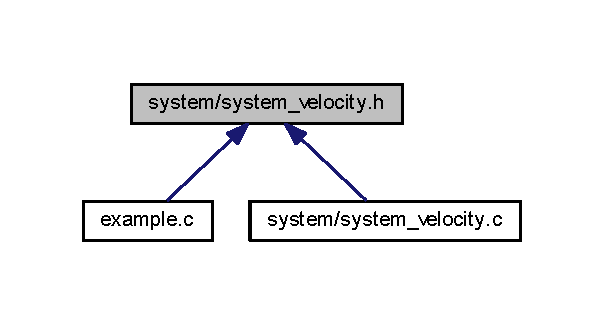
\includegraphics[width=290pt]{system__velocity_8h__dep__incl}
\end{center}
\end{figure}
\subsection*{Functions}
\begin{DoxyCompactItemize}
\item 
void \mbox{\hyperlink{system__velocity_8h_a9b052269b4956842d12134a81e066d81}{add\+\_\+velocity}} (\mbox{\hyperlink{struct_position_component_pool}{Position\+Component\+Pool}} $\ast$position\+\_\+component\+\_\+pool, \mbox{\hyperlink{struct_velocity_component_pool}{Velocity\+Component\+Pool}} $\ast$velocity\+\_\+component\+\_\+pool)
\end{DoxyCompactItemize}


\subsection{Function Documentation}
\mbox{\Hypertarget{system__velocity_8h_a9b052269b4956842d12134a81e066d81}\label{system__velocity_8h_a9b052269b4956842d12134a81e066d81}} 
\index{system\+\_\+velocity.\+h@{system\+\_\+velocity.\+h}!add\+\_\+velocity@{add\+\_\+velocity}}
\index{add\+\_\+velocity@{add\+\_\+velocity}!system\+\_\+velocity.\+h@{system\+\_\+velocity.\+h}}
\subsubsection{\texorpdfstring{add\+\_\+velocity()}{add\_velocity()}}
{\footnotesize\ttfamily void add\+\_\+velocity (\begin{DoxyParamCaption}\item[{\mbox{\hyperlink{struct_position_component_pool}{Position\+Component\+Pool}} $\ast$}]{position\+\_\+component\+\_\+pool,  }\item[{\mbox{\hyperlink{struct_velocity_component_pool}{Velocity\+Component\+Pool}} $\ast$}]{velocity\+\_\+component\+\_\+pool }\end{DoxyParamCaption})}

Here is the caller graph for this function\+:\nopagebreak
\begin{figure}[H]
\begin{center}
\leavevmode
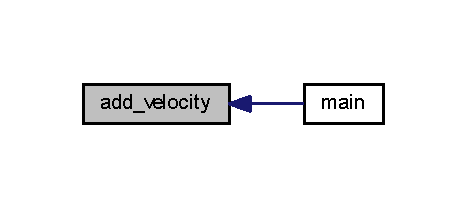
\includegraphics[width=224pt]{system__velocity_8h_a9b052269b4956842d12134a81e066d81_icgraph}
\end{center}
\end{figure}

\hypertarget{assemblage_8h}{}\section{assemblage.\+h File Reference}
\label{assemblage_8h}\index{assemblage.\+h@{assemblage.\+h}}
This graph shows which files directly or indirectly include this file\+:\nopagebreak
\begin{figure}[H]
\begin{center}
\leavevmode
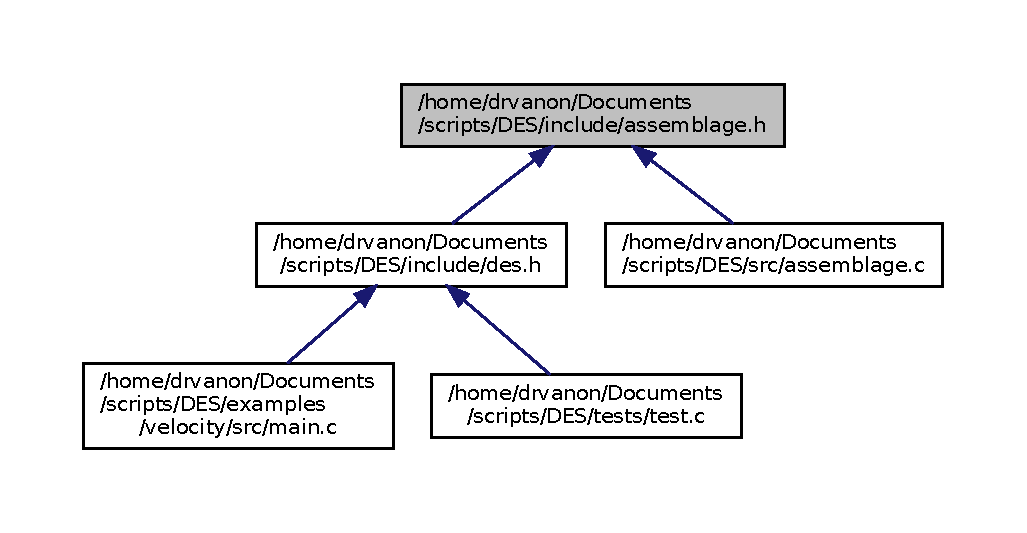
\includegraphics[width=157pt]{assemblage_8h__dep__incl}
\end{center}
\end{figure}
\subsection*{Functions}
\begin{DoxyCompactItemize}
\item 
int \mbox{\hyperlink{assemblage_8h_afc736eff8f29c778a8ecff259e7608a9}{assemblage\+\_\+create}} ()
\begin{DoxyCompactList}\small\item\em Create a new assemblage. \end{DoxyCompactList}\item 
int \mbox{\hyperlink{assemblage_8h_aec35c8cc69f98525ae6406f687259673}{assemblage\+\_\+row\+\_\+find\+\_\+empty}} ()
\begin{DoxyCompactList}\small\item\em Find an empty row in the assemblage table. \end{DoxyCompactList}\item 
int \mbox{\hyperlink{assemblage_8h_a668b0d6cb0ce05fe8b975d1549e18049}{assemblage\+\_\+register\+\_\+component}} (int assemblage\+\_\+id, \mbox{\hyperlink{struct_meta_component_pool}{Meta\+Component\+Pool}} $\ast$component)
\begin{DoxyCompactList}\small\item\em Create a entry in the assemablage table. \end{DoxyCompactList}\item 
int \mbox{\hyperlink{assemblage_8h_a075483752fba32efb629c3bf3df65279}{assemblage\+\_\+remove\+\_\+component}} (int assemblage\+\_\+id, \mbox{\hyperlink{struct_meta_component_pool}{Meta\+Component\+Pool}} $\ast$component)
\begin{DoxyCompactList}\small\item\em Remove a component from an assemblage. \end{DoxyCompactList}\item 
int \mbox{\hyperlink{assemblage_8h_a8824f5dc055fa00237c2ca883a855de7}{assemblage\+\_\+create\+\_\+entity}} (\mbox{\hyperlink{struct_entity_pool}{Entity\+Pool}} $\ast$entity\+\_\+pool, int assemblage\+\_\+id)
\begin{DoxyCompactList}\small\item\em Create a new entity in the provided \mbox{\hyperlink{struct_entity_pool}{Entity\+Pool}} from the assemblage that is identified by the assemblage\+\_\+id. \end{DoxyCompactList}\end{DoxyCompactItemize}


\subsection{Function Documentation}
\mbox{\Hypertarget{assemblage_8h_afc736eff8f29c778a8ecff259e7608a9}\label{assemblage_8h_afc736eff8f29c778a8ecff259e7608a9}} 
\index{assemblage.\+h@{assemblage.\+h}!assemblage\+\_\+create@{assemblage\+\_\+create}}
\index{assemblage\+\_\+create@{assemblage\+\_\+create}!assemblage.\+h@{assemblage.\+h}}
\subsubsection{\texorpdfstring{assemblage\+\_\+create()}{assemblage\_create()}}
{\footnotesize\ttfamily int assemblage\+\_\+create (\begin{DoxyParamCaption}{ }\end{DoxyParamCaption})}



Create a new assemblage. 

\begin{DoxyReturn}{Returns}
int The new assemblage\+\_\+id 
\end{DoxyReturn}
\mbox{\Hypertarget{assemblage_8h_a8824f5dc055fa00237c2ca883a855de7}\label{assemblage_8h_a8824f5dc055fa00237c2ca883a855de7}} 
\index{assemblage.\+h@{assemblage.\+h}!assemblage\+\_\+create\+\_\+entity@{assemblage\+\_\+create\+\_\+entity}}
\index{assemblage\+\_\+create\+\_\+entity@{assemblage\+\_\+create\+\_\+entity}!assemblage.\+h@{assemblage.\+h}}
\subsubsection{\texorpdfstring{assemblage\+\_\+create\+\_\+entity()}{assemblage\_create\_entity()}}
{\footnotesize\ttfamily int assemblage\+\_\+create\+\_\+entity (\begin{DoxyParamCaption}\item[{\mbox{\hyperlink{struct_entity_pool}{Entity\+Pool}} $\ast$}]{entity\+\_\+pool,  }\item[{int}]{assemblage\+\_\+id }\end{DoxyParamCaption})}



Create a new entity in the provided \mbox{\hyperlink{struct_entity_pool}{Entity\+Pool}} from the assemblage that is identified by the assemblage\+\_\+id. 


\begin{DoxyParams}{Parameters}
{\em entity\+\_\+pool} & \\
\hline
{\em assemblage\+\_\+id} & \\
\hline
\end{DoxyParams}
\begin{DoxyReturn}{Returns}
int G\+U\+ID of the newly created entity 
\end{DoxyReturn}
Here is the call graph for this function\+:\nopagebreak
\begin{figure}[H]
\begin{center}
\leavevmode
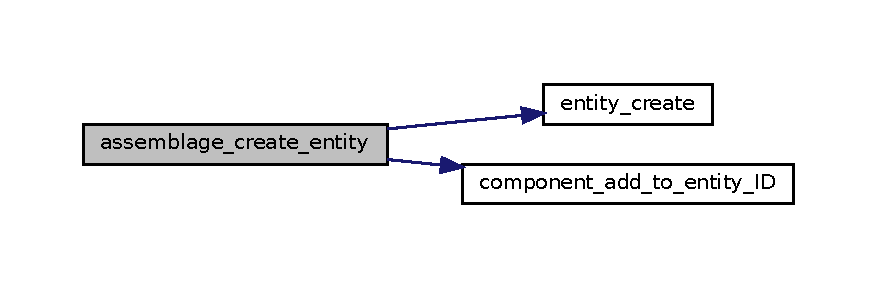
\includegraphics[width=350pt]{assemblage_8h_a8824f5dc055fa00237c2ca883a855de7_cgraph}
\end{center}
\end{figure}
\mbox{\Hypertarget{assemblage_8h_a668b0d6cb0ce05fe8b975d1549e18049}\label{assemblage_8h_a668b0d6cb0ce05fe8b975d1549e18049}} 
\index{assemblage.\+h@{assemblage.\+h}!assemblage\+\_\+register\+\_\+component@{assemblage\+\_\+register\+\_\+component}}
\index{assemblage\+\_\+register\+\_\+component@{assemblage\+\_\+register\+\_\+component}!assemblage.\+h@{assemblage.\+h}}
\subsubsection{\texorpdfstring{assemblage\+\_\+register\+\_\+component()}{assemblage\_register\_component()}}
{\footnotesize\ttfamily int assemblage\+\_\+register\+\_\+component (\begin{DoxyParamCaption}\item[{int}]{assemblage\+\_\+id,  }\item[{\mbox{\hyperlink{struct_meta_component_pool}{Meta\+Component\+Pool}} $\ast$}]{component }\end{DoxyParamCaption})}



Create a entry in the assemablage table. 


\begin{DoxyParams}{Parameters}
{\em assemblage\+\_\+id} & The assemblage id to which you wish to add the component \\
\hline
{\em component} & Pointer to the component pool that will be added to the newly created entity \\
\hline
\end{DoxyParams}
\begin{DoxyReturn}{Returns}
int Index that represents the row where the entry lives. 
\end{DoxyReturn}
Here is the call graph for this function\+:\nopagebreak
\begin{figure}[H]
\begin{center}
\leavevmode
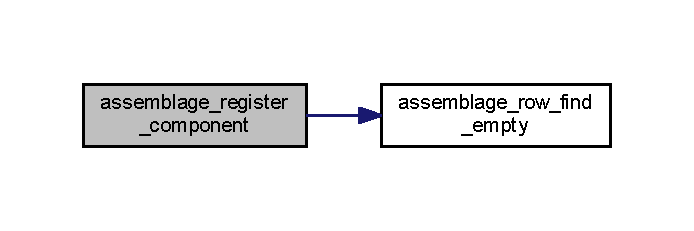
\includegraphics[width=333pt]{assemblage_8h_a668b0d6cb0ce05fe8b975d1549e18049_cgraph}
\end{center}
\end{figure}
\mbox{\Hypertarget{assemblage_8h_a075483752fba32efb629c3bf3df65279}\label{assemblage_8h_a075483752fba32efb629c3bf3df65279}} 
\index{assemblage.\+h@{assemblage.\+h}!assemblage\+\_\+remove\+\_\+component@{assemblage\+\_\+remove\+\_\+component}}
\index{assemblage\+\_\+remove\+\_\+component@{assemblage\+\_\+remove\+\_\+component}!assemblage.\+h@{assemblage.\+h}}
\subsubsection{\texorpdfstring{assemblage\+\_\+remove\+\_\+component()}{assemblage\_remove\_component()}}
{\footnotesize\ttfamily int assemblage\+\_\+remove\+\_\+component (\begin{DoxyParamCaption}\item[{int}]{assemblage\+\_\+id,  }\item[{\mbox{\hyperlink{struct_meta_component_pool}{Meta\+Component\+Pool}} $\ast$}]{component }\end{DoxyParamCaption})}



Remove a component from an assemblage. 


\begin{DoxyParams}{Parameters}
{\em assemblage\+\_\+id} & \\
\hline
{\em component} & \\
\hline
\end{DoxyParams}
\begin{DoxyReturn}{Returns}
int Error codes\+: 0 if okay, -\/1 if assemblage\+\_\+id out not in assemblage table. 
\end{DoxyReturn}
Here is the call graph for this function\+:\nopagebreak
\begin{figure}[H]
\begin{center}
\leavevmode
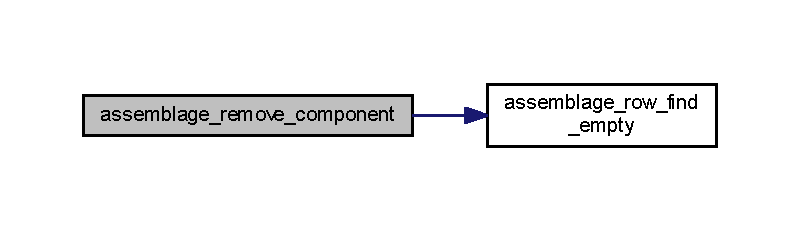
\includegraphics[width=350pt]{assemblage_8h_a075483752fba32efb629c3bf3df65279_cgraph}
\end{center}
\end{figure}
\mbox{\Hypertarget{assemblage_8h_aec35c8cc69f98525ae6406f687259673}\label{assemblage_8h_aec35c8cc69f98525ae6406f687259673}} 
\index{assemblage.\+h@{assemblage.\+h}!assemblage\+\_\+row\+\_\+find\+\_\+empty@{assemblage\+\_\+row\+\_\+find\+\_\+empty}}
\index{assemblage\+\_\+row\+\_\+find\+\_\+empty@{assemblage\+\_\+row\+\_\+find\+\_\+empty}!assemblage.\+h@{assemblage.\+h}}
\subsubsection{\texorpdfstring{assemblage\+\_\+row\+\_\+find\+\_\+empty()}{assemblage\_row\_find\_empty()}}
{\footnotesize\ttfamily int assemblage\+\_\+row\+\_\+find\+\_\+empty (\begin{DoxyParamCaption}{ }\end{DoxyParamCaption})}



Find an empty row in the assemblage table. 

\begin{DoxyReturn}{Returns}
int Index of the empty row. 
\end{DoxyReturn}
Here is the caller graph for this function\+:\nopagebreak
\begin{figure}[H]
\begin{center}
\leavevmode
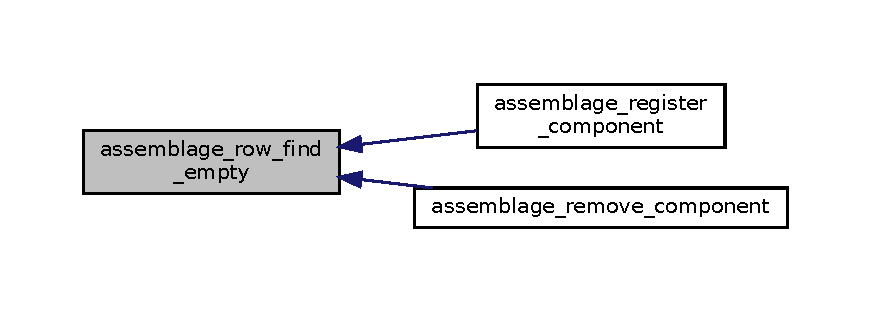
\includegraphics[width=350pt]{assemblage_8h_aec35c8cc69f98525ae6406f687259673_icgraph}
\end{center}
\end{figure}

\hypertarget{component_8h}{}\section{/home/drvanon/\+Documents/scripts/\+D\+E\+S/include/component.h File Reference}
\label{component_8h}\index{/home/drvanon/\+Documents/scripts/\+D\+E\+S/include/component.\+h@{/home/drvanon/\+Documents/scripts/\+D\+E\+S/include/component.\+h}}
This graph shows which files directly or indirectly include this file\+:\nopagebreak
\begin{figure}[H]
\begin{center}
\leavevmode
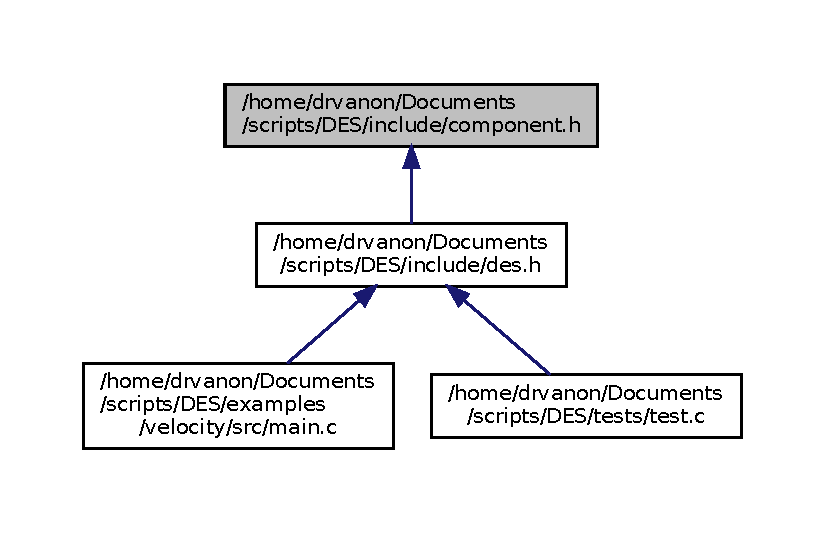
\includegraphics[width=350pt]{component_8h__dep__incl}
\end{center}
\end{figure}
\subsection*{Functions}
\begin{DoxyCompactItemize}
\item 
\mbox{\hyperlink{struct_entity_pool}{Entity\+Pool}} $\ast$ \mbox{\hyperlink{component_8h_a67e67b5444435172378a5e24701a02e7}{entity\+\_\+get\+\_\+components}} (\mbox{\hyperlink{struct_entity_pool}{Entity\+Pool}} $\ast$entity\+\_\+pool, int guid, int max\+\_\+query\+\_\+size)
\begin{DoxyCompactList}\small\item\em Retrieve upto max\+\_\+query\+\_\+size components linked to the entity in an \mbox{\hyperlink{struct_entity_pool}{Entity\+Pool}}. \end{DoxyCompactList}\item 
\mbox{\hyperlink{struct_meta_component_pool}{Meta\+Component\+Pool}} \mbox{\hyperlink{component_8h_ac9e98c2d8d4ef8d84bda94d824fbc7b0}{component\+\_\+pool\+\_\+register}} (void $\ast$component\+\_\+pool, int size)
\begin{DoxyCompactList}\small\item\em Register a component for use in the D\+ES system. \end{DoxyCompactList}\item 
int \mbox{\hyperlink{component_8h_a45e8d15e4080e8fb930e984fc9bac47a}{component\+\_\+add\+\_\+to\+\_\+entity\+\_\+\+ID}} (\mbox{\hyperlink{struct_entity_pool}{Entity\+Pool}} $\ast$entity\+\_\+pool, int guid, \mbox{\hyperlink{struct_meta_component_pool}{Meta\+Component\+Pool}} $\ast$meta\+\_\+component\+\_\+pool)
\begin{DoxyCompactList}\small\item\em Create a new row in the component-\/entity pool. \end{DoxyCompactList}\item 
int \mbox{\hyperlink{component_8h_a494f2d263a1053e2962e158f0a4c7e3a}{component\+\_\+add\+\_\+to\+\_\+entity\+\_\+index}} (\mbox{\hyperlink{struct_entity_pool}{Entity\+Pool}} $\ast$entity\+\_\+pool, int index, int guid, \mbox{\hyperlink{struct_meta_component_pool}{Meta\+Component\+Pool}} $\ast$meta\+\_\+component\+\_\+pool)
\begin{DoxyCompactList}\small\item\em Add a component to an entity if the user has already obtained an empty row. \end{DoxyCompactList}\item 
int \mbox{\hyperlink{component_8h_a46ad35b10ce23dc588b43f20fa5be2c2}{component\+\_\+remove\+\_\+from\+\_\+entity\+\_\+index}} (\mbox{\hyperlink{struct_entity_pool}{Entity\+Pool}} $\ast$entity\+\_\+pool, int index)
\begin{DoxyCompactList}\small\item\em Remove the row of the given index in the component-\/entity pool. \end{DoxyCompactList}\item 
int \mbox{\hyperlink{component_8h_af64e2220dd5596ce4f119c7887eac5c0}{component\+\_\+remove\+\_\+from\+\_\+entity\+\_\+\+ID}} (\mbox{\hyperlink{struct_entity_pool}{Entity\+Pool}} $\ast$entity\+\_\+pool, int guid, \mbox{\hyperlink{struct_meta_component_pool}{Meta\+Component\+Pool}} $\ast$meta\+\_\+component\+\_\+pool)
\begin{DoxyCompactList}\small\item\em Remove a single component from the specified entity. \end{DoxyCompactList}\item 
int \mbox{\hyperlink{component_8h_a997d5c45b99e95e34d3d00107eec6618}{component\+\_\+pool\+\_\+get\+\_\+open\+\_\+slot}} (\mbox{\hyperlink{struct_meta_component_pool}{Meta\+Component\+Pool}} $\ast$meta\+\_\+component\+\_\+pool)
\begin{DoxyCompactList}\small\item\em Find the first slot in the mask that has not been filled. \end{DoxyCompactList}\item 
int \mbox{\hyperlink{component_8h_a882c82b33bb428b62dab1b01c37e12a2}{component\+\_\+pool\+\_\+get\+\_\+slot}} (\mbox{\hyperlink{struct_meta_component_pool}{Meta\+Component\+Pool}} $\ast$meta\+\_\+component\+\_\+pool, int index)
\begin{DoxyCompactList}\small\item\em Find the state of a slot in a component pool. \end{DoxyCompactList}\item 
int \mbox{\hyperlink{component_8h_a1092fc1b1a8b8c021bc8e9dca328cf6c}{component\+\_\+pool\+\_\+set\+\_\+slot}} (\mbox{\hyperlink{struct_meta_component_pool}{Meta\+Component\+Pool}} $\ast$meta\+\_\+component\+\_\+pool, int index, int state)
\begin{DoxyCompactList}\small\item\em Set slot state in meta component to be vacant or free. \end{DoxyCompactList}\end{DoxyCompactItemize}


\subsection{Function Documentation}
\mbox{\Hypertarget{component_8h_a45e8d15e4080e8fb930e984fc9bac47a}\label{component_8h_a45e8d15e4080e8fb930e984fc9bac47a}} 
\index{component.\+h@{component.\+h}!component\+\_\+add\+\_\+to\+\_\+entity\+\_\+\+ID@{component\+\_\+add\+\_\+to\+\_\+entity\+\_\+\+ID}}
\index{component\+\_\+add\+\_\+to\+\_\+entity\+\_\+\+ID@{component\+\_\+add\+\_\+to\+\_\+entity\+\_\+\+ID}!component.\+h@{component.\+h}}
\subsubsection{\texorpdfstring{component\+\_\+add\+\_\+to\+\_\+entity\+\_\+\+I\+D()}{component\_add\_to\_entity\_ID()}}
{\footnotesize\ttfamily int component\+\_\+add\+\_\+to\+\_\+entity\+\_\+\+ID (\begin{DoxyParamCaption}\item[{\mbox{\hyperlink{struct_entity_pool}{Entity\+Pool}} $\ast$}]{entity\+\_\+pool,  }\item[{int}]{guid,  }\item[{\mbox{\hyperlink{struct_meta_component_pool}{Meta\+Component\+Pool}} $\ast$}]{meta\+\_\+component\+\_\+pool }\end{DoxyParamCaption})}



Create a new row in the component-\/entity pool. 

This function takes a previously established G\+U\+ID and a \mbox{\hyperlink{struct_meta_component_pool}{Meta\+Component\+Pool}} to create a new row in the component-\/entity pool. This is to be used in combination with create\+Entity, after having registered your component. 
\begin{DoxyCode}
\textcolor{keywordtype}{int} your\_component\_pool\_size = 200; \textcolor{comment}{// Amount of rows the componentPool can have}
EnityPool *entity\_pool = \mbox{\hyperlink{examples_2velocity_2include_2des_8h_a44b8855c1b56396b8faedcd389fe4546}{entity\_pool\_create}}(2000);
MetaComponentPoolPool YourMetaComponentPoolPool = component\_register(entity\_pool, *YourComponentPool, 
      your\_component\_pool\_size);
\textcolor{keywordtype}{int} guid = \mbox{\hyperlink{examples_2velocity_2include_2des_8h_ae84c376a8fb9ccf53cd54e0736e76eb2}{entity\_create}}();
\textcolor{keywordtype}{int} component\_index = \mbox{\hyperlink{examples_2velocity_2include_2des_8h_a45e8d15e4080e8fb930e984fc9bac47a}{component\_add\_to\_entity\_ID}}(guid, &YourMetaComponentPoolPool
      );
YourComponentPool.member1[component\_index] = \textcolor{stringliteral}{"Some content"};

\textcolor{comment}{// And after running the program:}
\mbox{\hyperlink{examples_2velocity_2include_2des_8h_a3e377867fe9b332352eb47cdf9dc1a4c}{entity\_pool\_destroy}}(entity\_pool);
free(YourComponent.member1);
free(YourComponent.member2); \textcolor{comment}{// etc.}
\end{DoxyCode}



\begin{DoxyParams}{Parameters}
{\em entity\+\_\+pool} & \\
\hline
{\em guid} & \\
\hline
{\em meta\+\_\+component\+\_\+pool} & \\
\hline
\end{DoxyParams}
\begin{DoxyReturn}{Returns}
int This variable refers to the index of the user defined component pool that can be set to the prefered data, see example above. 
\end{DoxyReturn}
Here is the call graph for this function\+:\nopagebreak
\begin{figure}[H]
\begin{center}
\leavevmode
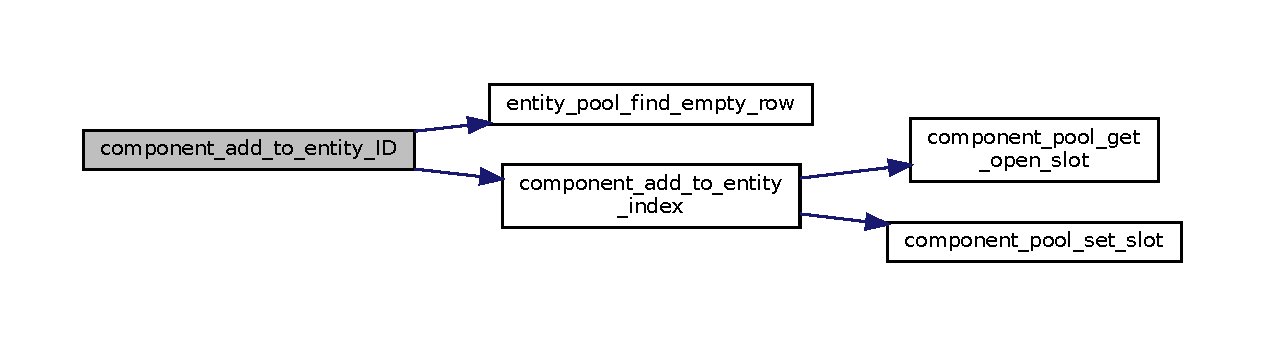
\includegraphics[width=350pt]{component_8h_a45e8d15e4080e8fb930e984fc9bac47a_cgraph}
\end{center}
\end{figure}
\mbox{\Hypertarget{component_8h_a494f2d263a1053e2962e158f0a4c7e3a}\label{component_8h_a494f2d263a1053e2962e158f0a4c7e3a}} 
\index{component.\+h@{component.\+h}!component\+\_\+add\+\_\+to\+\_\+entity\+\_\+index@{component\+\_\+add\+\_\+to\+\_\+entity\+\_\+index}}
\index{component\+\_\+add\+\_\+to\+\_\+entity\+\_\+index@{component\+\_\+add\+\_\+to\+\_\+entity\+\_\+index}!component.\+h@{component.\+h}}
\subsubsection{\texorpdfstring{component\+\_\+add\+\_\+to\+\_\+entity\+\_\+index()}{component\_add\_to\_entity\_index()}}
{\footnotesize\ttfamily int component\+\_\+add\+\_\+to\+\_\+entity\+\_\+index (\begin{DoxyParamCaption}\item[{\mbox{\hyperlink{struct_entity_pool}{Entity\+Pool}} $\ast$}]{entity\+\_\+pool,  }\item[{int}]{index,  }\item[{int}]{guid,  }\item[{\mbox{\hyperlink{struct_meta_component_pool}{Meta\+Component\+Pool}} $\ast$}]{meta\+\_\+component\+\_\+pool }\end{DoxyParamCaption})}



Add a component to an entity if the user has already obtained an empty row. 

It is possible that the user will be aware of the row that the entity was created in, so this is a copy of add\+\_\+component\+\_\+to\+\_\+entity\+\_\+\+ID, but works based of index instead of id, which is much faster, for we will not have to go trough the entire entity pool. An example for this might be inplace replacement of a row.


\begin{DoxyParams}{Parameters}
{\em entity\+\_\+pool} & \mbox{\hyperlink{struct_entity_pool}{Entity\+Pool}} in which to perform the action. \\
\hline
{\em index} & index of the entity-\/component pool \\
\hline
{\em guid} & guid of the new entity \\
\hline
{\em meta\+\_\+component\+\_\+pool} & \mbox{\hyperlink{struct_meta_component_pool}{Meta\+Component\+Pool}} of the component that is to be added to the entity \\
\hline
\end{DoxyParams}
\begin{DoxyReturn}{Returns}
int Index of component pool that can be used to store the data the user wants to store 
\end{DoxyReturn}
Here is the call graph for this function\+:\nopagebreak
\begin{figure}[H]
\begin{center}
\leavevmode
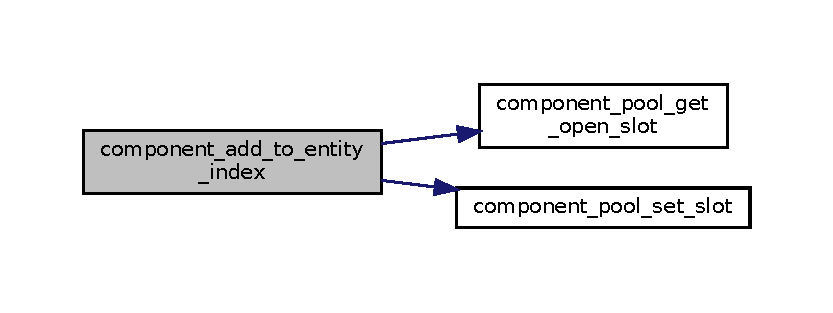
\includegraphics[width=350pt]{component_8h_a494f2d263a1053e2962e158f0a4c7e3a_cgraph}
\end{center}
\end{figure}
Here is the caller graph for this function\+:\nopagebreak
\begin{figure}[H]
\begin{center}
\leavevmode
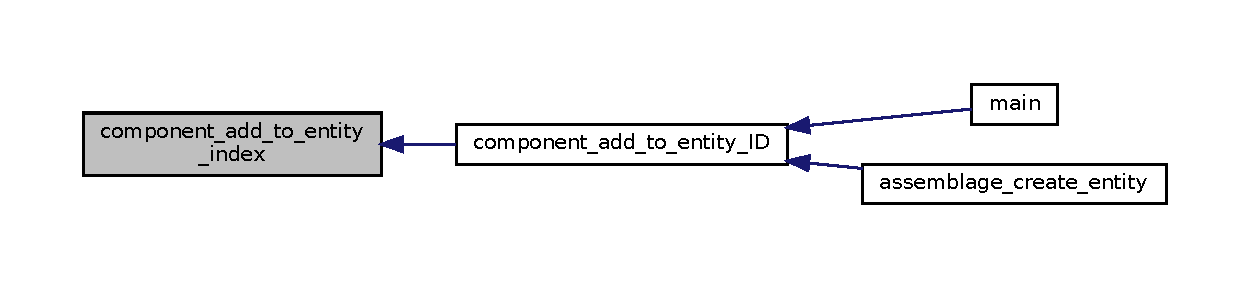
\includegraphics[width=350pt]{component_8h_a494f2d263a1053e2962e158f0a4c7e3a_icgraph}
\end{center}
\end{figure}
\mbox{\Hypertarget{component_8h_a997d5c45b99e95e34d3d00107eec6618}\label{component_8h_a997d5c45b99e95e34d3d00107eec6618}} 
\index{component.\+h@{component.\+h}!component\+\_\+pool\+\_\+get\+\_\+open\+\_\+slot@{component\+\_\+pool\+\_\+get\+\_\+open\+\_\+slot}}
\index{component\+\_\+pool\+\_\+get\+\_\+open\+\_\+slot@{component\+\_\+pool\+\_\+get\+\_\+open\+\_\+slot}!component.\+h@{component.\+h}}
\subsubsection{\texorpdfstring{component\+\_\+pool\+\_\+get\+\_\+open\+\_\+slot()}{component\_pool\_get\_open\_slot()}}
{\footnotesize\ttfamily int component\+\_\+pool\+\_\+get\+\_\+open\+\_\+slot (\begin{DoxyParamCaption}\item[{\mbox{\hyperlink{struct_meta_component_pool}{Meta\+Component\+Pool}} $\ast$}]{meta\+\_\+component\+\_\+pool }\end{DoxyParamCaption})}



Find the first slot in the mask that has not been filled. 


\begin{DoxyParams}{Parameters}
{\em meta\+\_\+component\+\_\+pool} & \\
\hline
\end{DoxyParams}
\begin{DoxyReturn}{Returns}
int component index of the open slot. 
\end{DoxyReturn}
\mbox{\Hypertarget{component_8h_a882c82b33bb428b62dab1b01c37e12a2}\label{component_8h_a882c82b33bb428b62dab1b01c37e12a2}} 
\index{component.\+h@{component.\+h}!component\+\_\+pool\+\_\+get\+\_\+slot@{component\+\_\+pool\+\_\+get\+\_\+slot}}
\index{component\+\_\+pool\+\_\+get\+\_\+slot@{component\+\_\+pool\+\_\+get\+\_\+slot}!component.\+h@{component.\+h}}
\subsubsection{\texorpdfstring{component\+\_\+pool\+\_\+get\+\_\+slot()}{component\_pool\_get\_slot()}}
{\footnotesize\ttfamily int component\+\_\+pool\+\_\+get\+\_\+slot (\begin{DoxyParamCaption}\item[{\mbox{\hyperlink{struct_meta_component_pool}{Meta\+Component\+Pool}} $\ast$}]{meta\+\_\+component\+\_\+pool,  }\item[{int}]{index }\end{DoxyParamCaption})}



Find the state of a slot in a component pool. 

This function will tell the user if the slot is in vacant or not.


\begin{DoxyParams}{Parameters}
{\em meta\+\_\+component\+\_\+pool} & \\
\hline
{\em index} & \\
\hline
\end{DoxyParams}
\begin{DoxyReturn}{Returns}
int bool value 
\end{DoxyReturn}
\mbox{\Hypertarget{component_8h_ac9e98c2d8d4ef8d84bda94d824fbc7b0}\label{component_8h_ac9e98c2d8d4ef8d84bda94d824fbc7b0}} 
\index{component.\+h@{component.\+h}!component\+\_\+pool\+\_\+register@{component\+\_\+pool\+\_\+register}}
\index{component\+\_\+pool\+\_\+register@{component\+\_\+pool\+\_\+register}!component.\+h@{component.\+h}}
\subsubsection{\texorpdfstring{component\+\_\+pool\+\_\+register()}{component\_pool\_register()}}
{\footnotesize\ttfamily \mbox{\hyperlink{struct_meta_component_pool}{Meta\+Component\+Pool}} component\+\_\+pool\+\_\+register (\begin{DoxyParamCaption}\item[{void $\ast$}]{component\+\_\+pool,  }\item[{int}]{size }\end{DoxyParamCaption})}



Register a component for use in the D\+ES system. 

The \mbox{\hyperlink{struct_meta_component_pool}{Meta\+Component\+Pool}} is used to provide an abstraction layer between the D\+ES and the user. It provides information on what index of the user defined component pool is open and what row is already in use by an entity. It also gives information on the size of the pool and refers to the component pool.


\begin{DoxyParams}{Parameters}
{\em component\+\_\+pool} & Pointer to the user-\/defined component\+\_\+pool. \\
\hline
{\em size} & Size of the memory allocated for the pools. \\
\hline
\end{DoxyParams}
\begin{DoxyReturn}{Returns}
\mbox{\hyperlink{struct_meta_component_pool}{Meta\+Component\+Pool}} 
\end{DoxyReturn}
\mbox{\Hypertarget{component_8h_a1092fc1b1a8b8c021bc8e9dca328cf6c}\label{component_8h_a1092fc1b1a8b8c021bc8e9dca328cf6c}} 
\index{component.\+h@{component.\+h}!component\+\_\+pool\+\_\+set\+\_\+slot@{component\+\_\+pool\+\_\+set\+\_\+slot}}
\index{component\+\_\+pool\+\_\+set\+\_\+slot@{component\+\_\+pool\+\_\+set\+\_\+slot}!component.\+h@{component.\+h}}
\subsubsection{\texorpdfstring{component\+\_\+pool\+\_\+set\+\_\+slot()}{component\_pool\_set\_slot()}}
{\footnotesize\ttfamily int component\+\_\+pool\+\_\+set\+\_\+slot (\begin{DoxyParamCaption}\item[{\mbox{\hyperlink{struct_meta_component_pool}{Meta\+Component\+Pool}} $\ast$}]{meta\+\_\+component\+\_\+pool,  }\item[{int}]{index,  }\item[{int}]{state }\end{DoxyParamCaption})}



Set slot state in meta component to be vacant or free. 


\begin{DoxyParams}{Parameters}
{\em meta\+\_\+component\+\_\+pool} & Meta of the component pool \\
\hline
{\em index} & Index of the slot \\
\hline
{\em state} & Desired state of the slot \\
\hline
\end{DoxyParams}
\begin{DoxyReturn}{Returns}
int Error codes\+: 0 is okay, -\/1 is index out of bounds 
\end{DoxyReturn}
\mbox{\Hypertarget{component_8h_af64e2220dd5596ce4f119c7887eac5c0}\label{component_8h_af64e2220dd5596ce4f119c7887eac5c0}} 
\index{component.\+h@{component.\+h}!component\+\_\+remove\+\_\+from\+\_\+entity\+\_\+\+ID@{component\+\_\+remove\+\_\+from\+\_\+entity\+\_\+\+ID}}
\index{component\+\_\+remove\+\_\+from\+\_\+entity\+\_\+\+ID@{component\+\_\+remove\+\_\+from\+\_\+entity\+\_\+\+ID}!component.\+h@{component.\+h}}
\subsubsection{\texorpdfstring{component\+\_\+remove\+\_\+from\+\_\+entity\+\_\+\+I\+D()}{component\_remove\_from\_entity\_ID()}}
{\footnotesize\ttfamily int component\+\_\+remove\+\_\+from\+\_\+entity\+\_\+\+ID (\begin{DoxyParamCaption}\item[{\mbox{\hyperlink{struct_entity_pool}{Entity\+Pool}} $\ast$}]{entity\+\_\+pool,  }\item[{int}]{guid,  }\item[{\mbox{\hyperlink{struct_meta_component_pool}{Meta\+Component\+Pool}} $\ast$}]{meta\+\_\+component\+\_\+pool }\end{DoxyParamCaption})}



Remove a single component from the specified entity. 


\begin{DoxyParams}{Parameters}
{\em entity\+\_\+pool} & \\
\hline
{\em guid} & \\
\hline
{\em meta\+\_\+component\+\_\+pool} & \\
\hline
\end{DoxyParams}
\begin{DoxyReturn}{Returns}
int Error codes\+: 0 is okay, -\/1 means could not find entity-\/component in pool. 
\end{DoxyReturn}
Here is the call graph for this function\+:\nopagebreak
\begin{figure}[H]
\begin{center}
\leavevmode
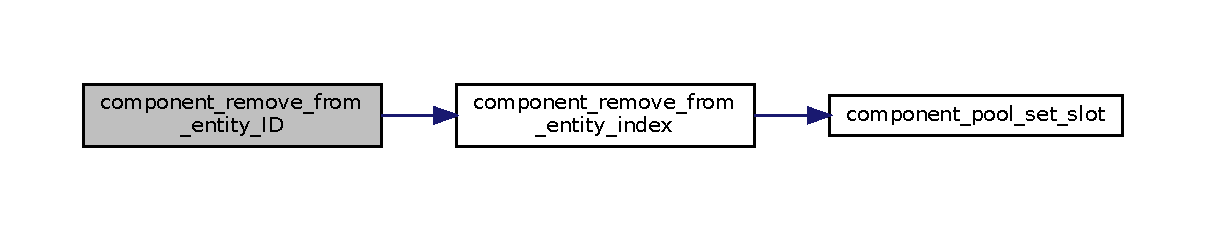
\includegraphics[width=350pt]{component_8h_af64e2220dd5596ce4f119c7887eac5c0_cgraph}
\end{center}
\end{figure}
\mbox{\Hypertarget{component_8h_a46ad35b10ce23dc588b43f20fa5be2c2}\label{component_8h_a46ad35b10ce23dc588b43f20fa5be2c2}} 
\index{component.\+h@{component.\+h}!component\+\_\+remove\+\_\+from\+\_\+entity\+\_\+index@{component\+\_\+remove\+\_\+from\+\_\+entity\+\_\+index}}
\index{component\+\_\+remove\+\_\+from\+\_\+entity\+\_\+index@{component\+\_\+remove\+\_\+from\+\_\+entity\+\_\+index}!component.\+h@{component.\+h}}
\subsubsection{\texorpdfstring{component\+\_\+remove\+\_\+from\+\_\+entity\+\_\+index()}{component\_remove\_from\_entity\_index()}}
{\footnotesize\ttfamily int component\+\_\+remove\+\_\+from\+\_\+entity\+\_\+index (\begin{DoxyParamCaption}\item[{\mbox{\hyperlink{struct_entity_pool}{Entity\+Pool}} $\ast$}]{entity\+\_\+pool,  }\item[{int}]{index }\end{DoxyParamCaption})}



Remove the row of the given index in the component-\/entity pool. 


\begin{DoxyParams}{Parameters}
{\em entity\+\_\+pool} & \\
\hline
{\em index} & \\
\hline
\end{DoxyParams}
\begin{DoxyReturn}{Returns}
int Error codes\+: 0 is okay, -\/1 is index out of bounds 
\end{DoxyReturn}
Here is the call graph for this function\+:\nopagebreak
\begin{figure}[H]
\begin{center}
\leavevmode
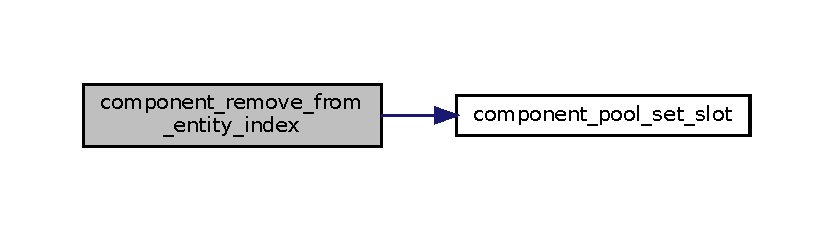
\includegraphics[width=350pt]{component_8h_a46ad35b10ce23dc588b43f20fa5be2c2_cgraph}
\end{center}
\end{figure}
Here is the caller graph for this function\+:\nopagebreak
\begin{figure}[H]
\begin{center}
\leavevmode
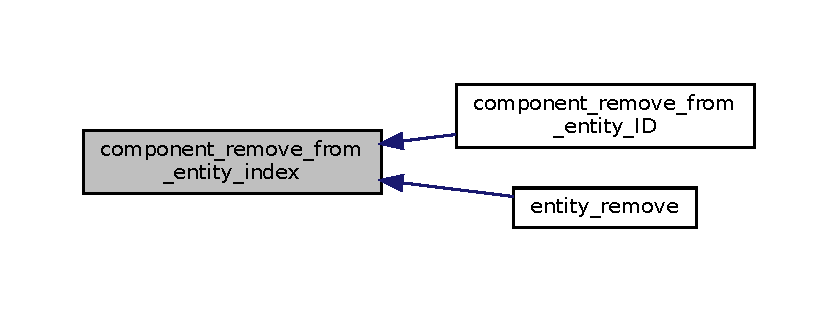
\includegraphics[width=350pt]{component_8h_a46ad35b10ce23dc588b43f20fa5be2c2_icgraph}
\end{center}
\end{figure}
\mbox{\Hypertarget{component_8h_a67e67b5444435172378a5e24701a02e7}\label{component_8h_a67e67b5444435172378a5e24701a02e7}} 
\index{component.\+h@{component.\+h}!entity\+\_\+get\+\_\+components@{entity\+\_\+get\+\_\+components}}
\index{entity\+\_\+get\+\_\+components@{entity\+\_\+get\+\_\+components}!component.\+h@{component.\+h}}
\subsubsection{\texorpdfstring{entity\+\_\+get\+\_\+components()}{entity\_get\_components()}}
{\footnotesize\ttfamily \mbox{\hyperlink{struct_entity_pool}{Entity\+Pool}}$\ast$ entity\+\_\+get\+\_\+components (\begin{DoxyParamCaption}\item[{\mbox{\hyperlink{struct_entity_pool}{Entity\+Pool}} $\ast$}]{entity\+\_\+pool,  }\item[{int}]{guid,  }\item[{int}]{max\+\_\+query\+\_\+size }\end{DoxyParamCaption})}



Retrieve upto max\+\_\+query\+\_\+size components linked to the entity in an \mbox{\hyperlink{struct_entity_pool}{Entity\+Pool}}. 


\begin{DoxyParams}{Parameters}
{\em entity\+\_\+pool} & \\
\hline
{\em guid} & \\
\hline
{\em max\+\_\+query\+\_\+size} & \\
\hline
\end{DoxyParams}
\begin{DoxyReturn}{Returns}
Entity\+Pool$\ast$ 
\end{DoxyReturn}
Here is the call graph for this function\+:\nopagebreak
\begin{figure}[H]
\begin{center}
\leavevmode
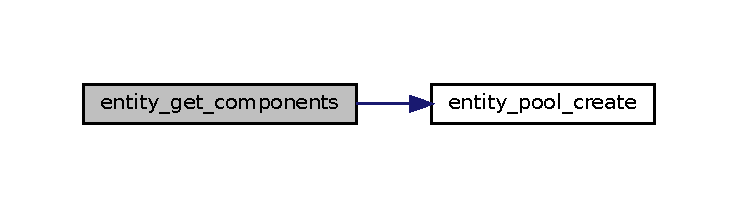
\includegraphics[width=350pt]{component_8h_a67e67b5444435172378a5e24701a02e7_cgraph}
\end{center}
\end{figure}

\hypertarget{entity_8h}{}\section{/home/drvanon/\+Documents/scripts/\+D\+E\+S/include/entity.h File Reference}
\label{entity_8h}\index{/home/drvanon/\+Documents/scripts/\+D\+E\+S/include/entity.\+h@{/home/drvanon/\+Documents/scripts/\+D\+E\+S/include/entity.\+h}}
{\ttfamily \#include \char`\"{}des\+\_\+internal.\+h\char`\"{}}\newline
Include dependency graph for entity.\+h\+:\nopagebreak
\begin{figure}[H]
\begin{center}
\leavevmode
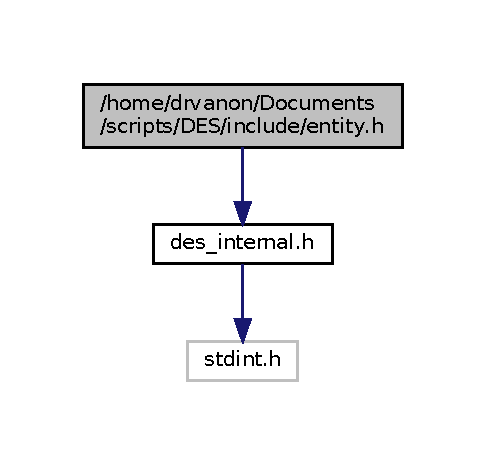
\includegraphics[width=233pt]{entity_8h__incl}
\end{center}
\end{figure}
This graph shows which files directly or indirectly include this file\+:\nopagebreak
\begin{figure}[H]
\begin{center}
\leavevmode
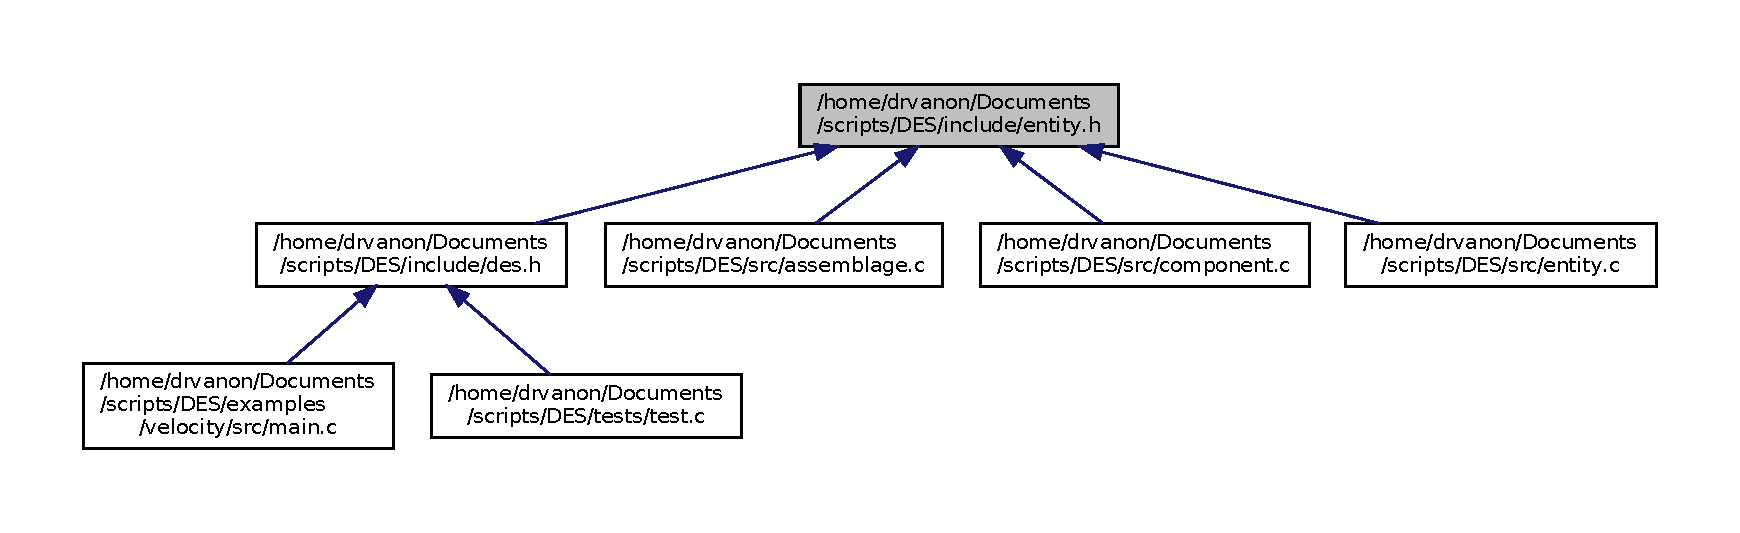
\includegraphics[width=350pt]{entity_8h__dep__incl}
\end{center}
\end{figure}
\subsection*{Data Structures}
\begin{DoxyCompactItemize}
\item 
struct \mbox{\hyperlink{struct_meta_component_pool}{Meta\+Component\+Pool}}
\begin{DoxyCompactList}\small\item\em Struct that creates a layer of abstraction between D\+ES and the user\textquotesingle{}s component pools. \end{DoxyCompactList}\item 
struct \mbox{\hyperlink{struct_entity_pool}{Entity\+Pool}}
\begin{DoxyCompactList}\small\item\em The pool that holds the entities and component relationships. \end{DoxyCompactList}\end{DoxyCompactItemize}
\subsection*{Typedefs}
\begin{DoxyCompactItemize}
\item 
typedef struct \mbox{\hyperlink{struct_meta_component_pool}{Meta\+Component\+Pool}} \mbox{\hyperlink{entity_8h_a0a09b6ff207d87cced8d3f986a50a101}{Meta\+Component\+Pool}}
\begin{DoxyCompactList}\small\item\em Struct that creates a layer of abstraction between D\+ES and the user\textquotesingle{}s component pools. \end{DoxyCompactList}\item 
typedef struct \mbox{\hyperlink{struct_entity_pool}{Entity\+Pool}} \mbox{\hyperlink{entity_8h_a629511a19dc302aaada724794387569d}{Entity\+Pool}}
\begin{DoxyCompactList}\small\item\em The pool that holds the entities and component relationships. \end{DoxyCompactList}\end{DoxyCompactItemize}
\subsection*{Functions}
\begin{DoxyCompactItemize}
\item 
\mbox{\hyperlink{struct_entity_pool}{Entity\+Pool}} $\ast$ \mbox{\hyperlink{entity_8h_a44b8855c1b56396b8faedcd389fe4546}{entity\+\_\+pool\+\_\+create}} (int size)
\begin{DoxyCompactList}\small\item\em Create \mbox{\hyperlink{struct_entity_pool}{Entity\+Pool}} and malloc it\textquotesingle{}s component with the size provided, returns N\+U\+LL if insufficient R\+AM. \end{DoxyCompactList}\item 
void \mbox{\hyperlink{entity_8h_a3e377867fe9b332352eb47cdf9dc1a4c}{entity\+\_\+pool\+\_\+destroy}} (\mbox{\hyperlink{struct_entity_pool}{Entity\+Pool}} $\ast$entity\+\_\+pool)
\begin{DoxyCompactList}\small\item\em Free all memory allocated for the \mbox{\hyperlink{struct_entity_pool}{Entity\+Pool}}. \end{DoxyCompactList}\item 
int \mbox{\hyperlink{entity_8h_a3955b16f45429c7ea74f275dac36493d}{entity\+\_\+pool\+\_\+find\+\_\+empty\+\_\+row}} (\mbox{\hyperlink{struct_entity_pool}{Entity\+Pool}} $\ast$entity\+\_\+pool)
\begin{DoxyCompactList}\small\item\em Find the index first empty row in the provided \mbox{\hyperlink{struct_entity_pool}{Entity\+Pool}}. \end{DoxyCompactList}\item 
int \mbox{\hyperlink{entity_8h_ae84c376a8fb9ccf53cd54e0736e76eb2}{entity\+\_\+create}} (\mbox{\hyperlink{struct_entity_pool}{Entity\+Pool}} $\ast$entity\+\_\+pool)
\begin{DoxyCompactList}\small\item\em Retrieve a new guid for an entity and register the change. \end{DoxyCompactList}\item 
void \mbox{\hyperlink{entity_8h_a7fa6d71c51a14d7607b66722a1f17427}{entity\+\_\+remove}} (\mbox{\hyperlink{struct_entity_pool}{Entity\+Pool}} $\ast$entity\+\_\+pool, int guid)
\begin{DoxyCompactList}\small\item\em Remove all data on the entity in the provided \mbox{\hyperlink{struct_entity_pool}{Entity\+Pool}}. \end{DoxyCompactList}\end{DoxyCompactItemize}


\subsection{Typedef Documentation}
\mbox{\Hypertarget{entity_8h_a629511a19dc302aaada724794387569d}\label{entity_8h_a629511a19dc302aaada724794387569d}} 
\index{entity.\+h@{entity.\+h}!Entity\+Pool@{Entity\+Pool}}
\index{Entity\+Pool@{Entity\+Pool}!entity.\+h@{entity.\+h}}
\subsubsection{\texorpdfstring{Entity\+Pool}{EntityPool}}
{\footnotesize\ttfamily typedef struct \mbox{\hyperlink{struct_entity_pool}{Entity\+Pool}}  \mbox{\hyperlink{struct_entity_pool}{Entity\+Pool}}}



The pool that holds the entities and component relationships. 

\mbox{\Hypertarget{entity_8h_a0a09b6ff207d87cced8d3f986a50a101}\label{entity_8h_a0a09b6ff207d87cced8d3f986a50a101}} 
\index{entity.\+h@{entity.\+h}!Meta\+Component\+Pool@{Meta\+Component\+Pool}}
\index{Meta\+Component\+Pool@{Meta\+Component\+Pool}!entity.\+h@{entity.\+h}}
\subsubsection{\texorpdfstring{Meta\+Component\+Pool}{MetaComponentPool}}
{\footnotesize\ttfamily typedef struct \mbox{\hyperlink{struct_meta_component_pool}{Meta\+Component\+Pool}}  \mbox{\hyperlink{struct_meta_component_pool}{Meta\+Component\+Pool}}}



Struct that creates a layer of abstraction between D\+ES and the user\textquotesingle{}s component pools. 



\subsection{Function Documentation}
\mbox{\Hypertarget{entity_8h_ae84c376a8fb9ccf53cd54e0736e76eb2}\label{entity_8h_ae84c376a8fb9ccf53cd54e0736e76eb2}} 
\index{entity.\+h@{entity.\+h}!entity\+\_\+create@{entity\+\_\+create}}
\index{entity\+\_\+create@{entity\+\_\+create}!entity.\+h@{entity.\+h}}
\subsubsection{\texorpdfstring{entity\+\_\+create()}{entity\_create()}}
{\footnotesize\ttfamily int entity\+\_\+create (\begin{DoxyParamCaption}\item[{\mbox{\hyperlink{struct_entity_pool}{Entity\+Pool}} $\ast$}]{entity\+\_\+pool }\end{DoxyParamCaption})}



Retrieve a new guid for an entity and register the change. 


\begin{DoxyParams}{Parameters}
{\em entity\+\_\+pool} & \\
\hline
\end{DoxyParams}
\begin{DoxyReturn}{Returns}
int 
\end{DoxyReturn}
Here is the call graph for this function\+:\nopagebreak
\begin{figure}[H]
\begin{center}
\leavevmode
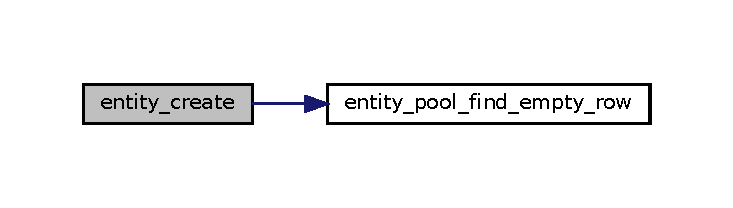
\includegraphics[width=350pt]{entity_8h_ae84c376a8fb9ccf53cd54e0736e76eb2_cgraph}
\end{center}
\end{figure}
\mbox{\Hypertarget{entity_8h_a44b8855c1b56396b8faedcd389fe4546}\label{entity_8h_a44b8855c1b56396b8faedcd389fe4546}} 
\index{entity.\+h@{entity.\+h}!entity\+\_\+pool\+\_\+create@{entity\+\_\+pool\+\_\+create}}
\index{entity\+\_\+pool\+\_\+create@{entity\+\_\+pool\+\_\+create}!entity.\+h@{entity.\+h}}
\subsubsection{\texorpdfstring{entity\+\_\+pool\+\_\+create()}{entity\_pool\_create()}}
{\footnotesize\ttfamily \mbox{\hyperlink{struct_entity_pool}{Entity\+Pool}}$\ast$ entity\+\_\+pool\+\_\+create (\begin{DoxyParamCaption}\item[{int}]{size }\end{DoxyParamCaption})}



Create \mbox{\hyperlink{struct_entity_pool}{Entity\+Pool}} and malloc it\textquotesingle{}s component with the size provided, returns N\+U\+LL if insufficient R\+AM. 


\begin{DoxyParams}{Parameters}
{\em size} & \\
\hline
\end{DoxyParams}
\begin{DoxyReturn}{Returns}
Entity\+Pool$\ast$ 
\end{DoxyReturn}
Here is the call graph for this function\+:\nopagebreak
\begin{figure}[H]
\begin{center}
\leavevmode
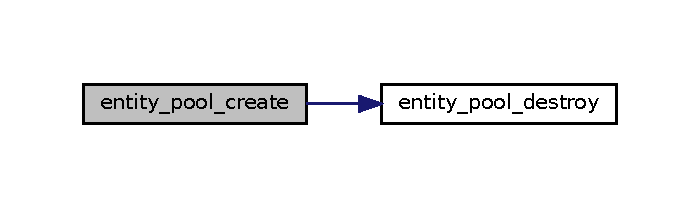
\includegraphics[width=336pt]{entity_8h_a44b8855c1b56396b8faedcd389fe4546_cgraph}
\end{center}
\end{figure}
\mbox{\Hypertarget{entity_8h_a3e377867fe9b332352eb47cdf9dc1a4c}\label{entity_8h_a3e377867fe9b332352eb47cdf9dc1a4c}} 
\index{entity.\+h@{entity.\+h}!entity\+\_\+pool\+\_\+destroy@{entity\+\_\+pool\+\_\+destroy}}
\index{entity\+\_\+pool\+\_\+destroy@{entity\+\_\+pool\+\_\+destroy}!entity.\+h@{entity.\+h}}
\subsubsection{\texorpdfstring{entity\+\_\+pool\+\_\+destroy()}{entity\_pool\_destroy()}}
{\footnotesize\ttfamily void entity\+\_\+pool\+\_\+destroy (\begin{DoxyParamCaption}\item[{\mbox{\hyperlink{struct_entity_pool}{Entity\+Pool}} $\ast$}]{entity\+\_\+pool }\end{DoxyParamCaption})}



Free all memory allocated for the \mbox{\hyperlink{struct_entity_pool}{Entity\+Pool}}. 


\begin{DoxyParams}{Parameters}
{\em entity\+\_\+pool} & \\
\hline
\end{DoxyParams}
Here is the caller graph for this function\+:\nopagebreak
\begin{figure}[H]
\begin{center}
\leavevmode
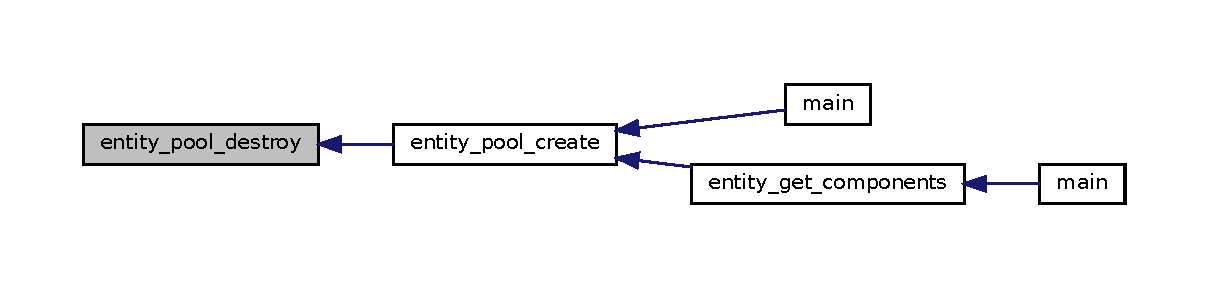
\includegraphics[width=350pt]{entity_8h_a3e377867fe9b332352eb47cdf9dc1a4c_icgraph}
\end{center}
\end{figure}
\mbox{\Hypertarget{entity_8h_a3955b16f45429c7ea74f275dac36493d}\label{entity_8h_a3955b16f45429c7ea74f275dac36493d}} 
\index{entity.\+h@{entity.\+h}!entity\+\_\+pool\+\_\+find\+\_\+empty\+\_\+row@{entity\+\_\+pool\+\_\+find\+\_\+empty\+\_\+row}}
\index{entity\+\_\+pool\+\_\+find\+\_\+empty\+\_\+row@{entity\+\_\+pool\+\_\+find\+\_\+empty\+\_\+row}!entity.\+h@{entity.\+h}}
\subsubsection{\texorpdfstring{entity\+\_\+pool\+\_\+find\+\_\+empty\+\_\+row()}{entity\_pool\_find\_empty\_row()}}
{\footnotesize\ttfamily int entity\+\_\+pool\+\_\+find\+\_\+empty\+\_\+row (\begin{DoxyParamCaption}\item[{\mbox{\hyperlink{struct_entity_pool}{Entity\+Pool}} $\ast$}]{entity\+\_\+pool }\end{DoxyParamCaption})}



Find the index first empty row in the provided \mbox{\hyperlink{struct_entity_pool}{Entity\+Pool}}. 


\begin{DoxyParams}{Parameters}
{\em entity\+\_\+pool} & \\
\hline
\end{DoxyParams}
\begin{DoxyReturn}{Returns}
int 
\end{DoxyReturn}
Here is the caller graph for this function\+:\nopagebreak
\begin{figure}[H]
\begin{center}
\leavevmode
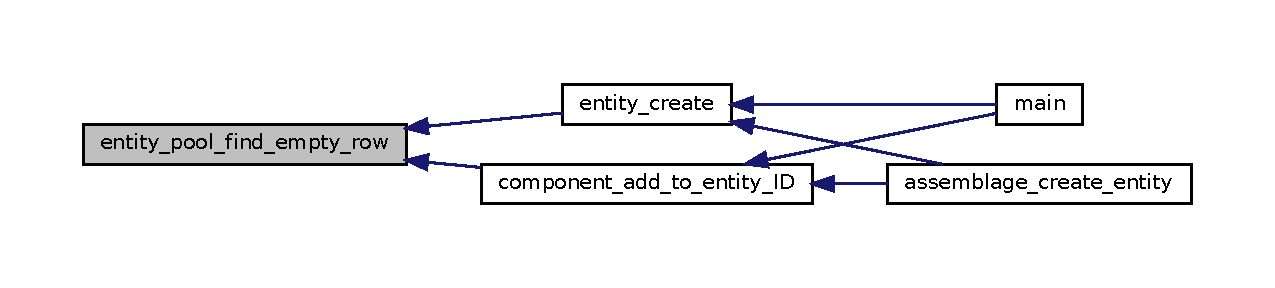
\includegraphics[width=350pt]{entity_8h_a3955b16f45429c7ea74f275dac36493d_icgraph}
\end{center}
\end{figure}
\mbox{\Hypertarget{entity_8h_a7fa6d71c51a14d7607b66722a1f17427}\label{entity_8h_a7fa6d71c51a14d7607b66722a1f17427}} 
\index{entity.\+h@{entity.\+h}!entity\+\_\+remove@{entity\+\_\+remove}}
\index{entity\+\_\+remove@{entity\+\_\+remove}!entity.\+h@{entity.\+h}}
\subsubsection{\texorpdfstring{entity\+\_\+remove()}{entity\_remove()}}
{\footnotesize\ttfamily void entity\+\_\+remove (\begin{DoxyParamCaption}\item[{\mbox{\hyperlink{struct_entity_pool}{Entity\+Pool}} $\ast$}]{entity\+\_\+pool,  }\item[{int}]{guid }\end{DoxyParamCaption})}



Remove all data on the entity in the provided \mbox{\hyperlink{struct_entity_pool}{Entity\+Pool}}. 


\begin{DoxyParams}{Parameters}
{\em entity\+\_\+pool} & \\
\hline
{\em guid} & \\
\hline
\end{DoxyParams}
Here is the call graph for this function\+:\nopagebreak
\begin{figure}[H]
\begin{center}
\leavevmode
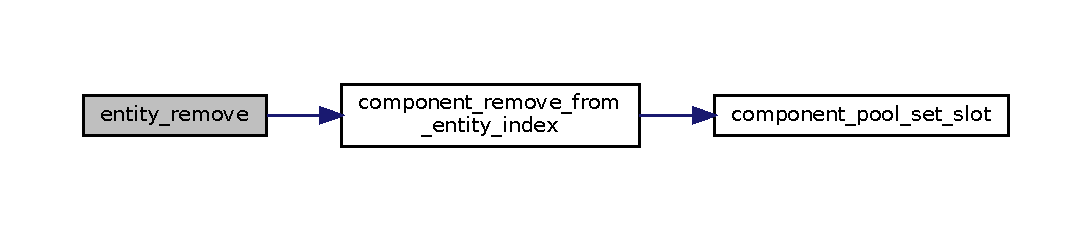
\includegraphics[width=350pt]{entity_8h_a7fa6d71c51a14d7607b66722a1f17427_cgraph}
\end{center}
\end{figure}

\hypertarget{assemblage_8o_8d}{}\section{/home/drvanon/\+Documents/scripts/\+D\+E\+S/obj/src/assemblage.o.\+d File Reference}
\label{assemblage_8o_8d}\index{/home/drvanon/\+Documents/scripts/\+D\+E\+S/obj/src/assemblage.\+o.\+d@{/home/drvanon/\+Documents/scripts/\+D\+E\+S/obj/src/assemblage.\+o.\+d}}

\hypertarget{component_8o_8d}{}\section{/home/drvanon/\+Documents/scripts/\+D\+E\+S/obj/src/component.o.\+d File Reference}
\label{component_8o_8d}\index{/home/drvanon/\+Documents/scripts/\+D\+E\+S/obj/src/component.\+o.\+d@{/home/drvanon/\+Documents/scripts/\+D\+E\+S/obj/src/component.\+o.\+d}}

\hypertarget{des_8o_8d}{}\section{/home/drvanon/\+Documents/scripts/\+D\+E\+S/obj/src/des.o.\+d File Reference}
\label{des_8o_8d}\index{/home/drvanon/\+Documents/scripts/\+D\+E\+S/obj/src/des.\+o.\+d@{/home/drvanon/\+Documents/scripts/\+D\+E\+S/obj/src/des.\+o.\+d}}

\hypertarget{entity_8o_8d}{}\section{/home/drvanon/\+Documents/scripts/\+D\+E\+S/obj/src/entity.o.\+d File Reference}
\label{entity_8o_8d}\index{/home/drvanon/\+Documents/scripts/\+D\+E\+S/obj/src/entity.\+o.\+d@{/home/drvanon/\+Documents/scripts/\+D\+E\+S/obj/src/entity.\+o.\+d}}

\hypertarget{obj_2src_2tests_2test_8o_8d}{}\section{/home/drvanon/\+Documents/scripts/\+D\+E\+S/obj/src/tests/test.o.\+d File Reference}
\label{obj_2src_2tests_2test_8o_8d}\index{/home/drvanon/\+Documents/scripts/\+D\+E\+S/obj/src/tests/test.\+o.\+d@{/home/drvanon/\+Documents/scripts/\+D\+E\+S/obj/src/tests/test.\+o.\+d}}

\hypertarget{tests_2obj_2test_8o_8d}{}\section{/home/drvanon/\+Documents/scripts/\+D\+E\+S/tests/obj/test.o.\+d File Reference}
\label{tests_2obj_2test_8o_8d}\index{/home/drvanon/\+Documents/scripts/\+D\+E\+S/tests/obj/test.\+o.\+d@{/home/drvanon/\+Documents/scripts/\+D\+E\+S/tests/obj/test.\+o.\+d}}

\hypertarget{_r_e_a_d_m_e_8md}{}\section{R\+E\+A\+D\+M\+E.\+md File Reference}
\label{_r_e_a_d_m_e_8md}\index{R\+E\+A\+D\+M\+E.\+md@{R\+E\+A\+D\+M\+E.\+md}}

\hypertarget{assemblage_8c}{}\section{/home/drvanon/\+Documents/scripts/\+D\+E\+S/src/assemblage.c File Reference}
\label{assemblage_8c}\index{/home/drvanon/\+Documents/scripts/\+D\+E\+S/src/assemblage.\+c@{/home/drvanon/\+Documents/scripts/\+D\+E\+S/src/assemblage.\+c}}
{\ttfamily \#include \char`\"{}entity.\+h\char`\"{}}\newline
{\ttfamily \#include \char`\"{}assemblage.\+h\char`\"{}}\newline
Include dependency graph for assemblage.\+c\+:\nopagebreak
\begin{figure}[H]
\begin{center}
\leavevmode
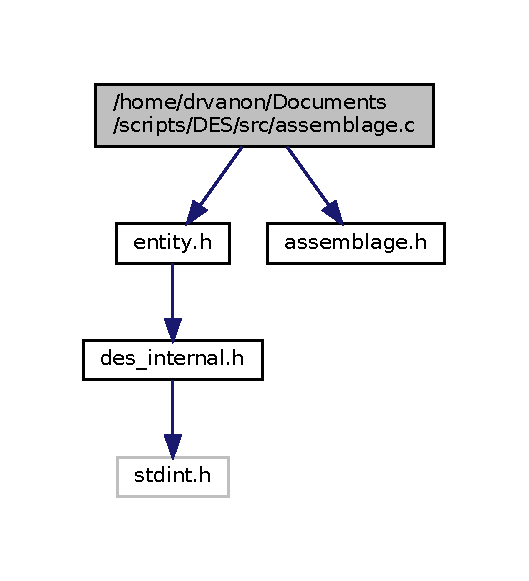
\includegraphics[width=254pt]{assemblage_8c__incl}
\end{center}
\end{figure}
\subsection*{Data Structures}
\begin{DoxyCompactItemize}
\item 
struct \mbox{\hyperlink{struct_assemblage_pool}{Assemblage\+Pool}}
\begin{DoxyCompactList}\small\item\em Assemblage pool. \end{DoxyCompactList}\end{DoxyCompactItemize}
\subsection*{Macros}
\begin{DoxyCompactItemize}
\item 
\#define \mbox{\hyperlink{assemblage_8c_a7278dc587e6d944803677e7662c25147}{A\+S\+S\+E\+M\+B\+L\+A\+G\+E\+\_\+\+P\+O\+O\+L\+\_\+\+S\+I\+ZE}}~100
\end{DoxyCompactItemize}
\subsection*{Typedefs}
\begin{DoxyCompactItemize}
\item 
typedef struct \mbox{\hyperlink{struct_assemblage_pool}{Assemblage\+Pool}} \mbox{\hyperlink{assemblage_8c_a800d18985dee1a39b3e212d06ed10fa8}{Assemblage\+Pool}}
\begin{DoxyCompactList}\small\item\em Assemblage pool. \end{DoxyCompactList}\end{DoxyCompactItemize}
\subsection*{Functions}
\begin{DoxyCompactItemize}
\item 
int \mbox{\hyperlink{assemblage_8c_aec35c8cc69f98525ae6406f687259673}{assemblage\+\_\+row\+\_\+find\+\_\+empty}} ()
\begin{DoxyCompactList}\small\item\em Find an empty row in the assemblage table. \end{DoxyCompactList}\item 
int \mbox{\hyperlink{assemblage_8c_afc736eff8f29c778a8ecff259e7608a9}{assemblage\+\_\+create}} ()
\begin{DoxyCompactList}\small\item\em Create a new assemblage. \end{DoxyCompactList}\item 
int \mbox{\hyperlink{assemblage_8c_a668b0d6cb0ce05fe8b975d1549e18049}{assemblage\+\_\+register\+\_\+component}} (int assemblage\+\_\+id, \mbox{\hyperlink{struct_meta_component_pool}{Meta\+Component\+Pool}} $\ast$component)
\begin{DoxyCompactList}\small\item\em Create a entry in the assemablage table. \end{DoxyCompactList}\item 
int \mbox{\hyperlink{assemblage_8c_a075483752fba32efb629c3bf3df65279}{assemblage\+\_\+remove\+\_\+component}} (int assemblage\+\_\+id, \mbox{\hyperlink{struct_meta_component_pool}{Meta\+Component\+Pool}} $\ast$component)
\begin{DoxyCompactList}\small\item\em Remove a component from an assemblage. \end{DoxyCompactList}\item 
int \mbox{\hyperlink{assemblage_8c_a8824f5dc055fa00237c2ca883a855de7}{assemblage\+\_\+create\+\_\+entity}} (\mbox{\hyperlink{struct_entity_pool}{Entity\+Pool}} $\ast$entity\+\_\+pool, int assemblage\+\_\+id)
\begin{DoxyCompactList}\small\item\em Create a new entity in the provided \mbox{\hyperlink{struct_entity_pool}{Entity\+Pool}} from the assemblage that is identified by the assemblage\+\_\+id. \end{DoxyCompactList}\end{DoxyCompactItemize}
\subsection*{Variables}
\begin{DoxyCompactItemize}
\item 
\mbox{\hyperlink{struct_assemblage_pool}{Assemblage\+Pool}} \mbox{\hyperlink{assemblage_8c_abef5ea0528d8e5d61219208774e36465}{A\+S\+S\+E\+M\+B\+L\+A\+G\+E\+\_\+\+P\+O\+OL}}
\end{DoxyCompactItemize}


\subsection{Macro Definition Documentation}
\mbox{\Hypertarget{assemblage_8c_a7278dc587e6d944803677e7662c25147}\label{assemblage_8c_a7278dc587e6d944803677e7662c25147}} 
\index{assemblage.\+c@{assemblage.\+c}!A\+S\+S\+E\+M\+B\+L\+A\+G\+E\+\_\+\+P\+O\+O\+L\+\_\+\+S\+I\+ZE@{A\+S\+S\+E\+M\+B\+L\+A\+G\+E\+\_\+\+P\+O\+O\+L\+\_\+\+S\+I\+ZE}}
\index{A\+S\+S\+E\+M\+B\+L\+A\+G\+E\+\_\+\+P\+O\+O\+L\+\_\+\+S\+I\+ZE@{A\+S\+S\+E\+M\+B\+L\+A\+G\+E\+\_\+\+P\+O\+O\+L\+\_\+\+S\+I\+ZE}!assemblage.\+c@{assemblage.\+c}}
\subsubsection{\texorpdfstring{A\+S\+S\+E\+M\+B\+L\+A\+G\+E\+\_\+\+P\+O\+O\+L\+\_\+\+S\+I\+ZE}{ASSEMBLAGE\_POOL\_SIZE}}
{\footnotesize\ttfamily \#define A\+S\+S\+E\+M\+B\+L\+A\+G\+E\+\_\+\+P\+O\+O\+L\+\_\+\+S\+I\+ZE~100}



\subsection{Typedef Documentation}
\mbox{\Hypertarget{assemblage_8c_a800d18985dee1a39b3e212d06ed10fa8}\label{assemblage_8c_a800d18985dee1a39b3e212d06ed10fa8}} 
\index{assemblage.\+c@{assemblage.\+c}!Assemblage\+Pool@{Assemblage\+Pool}}
\index{Assemblage\+Pool@{Assemblage\+Pool}!assemblage.\+c@{assemblage.\+c}}
\subsubsection{\texorpdfstring{Assemblage\+Pool}{AssemblagePool}}
{\footnotesize\ttfamily typedef struct \mbox{\hyperlink{struct_assemblage_pool}{Assemblage\+Pool}}  \mbox{\hyperlink{struct_assemblage_pool}{Assemblage\+Pool}}}



Assemblage pool. 



\subsection{Function Documentation}
\mbox{\Hypertarget{assemblage_8c_afc736eff8f29c778a8ecff259e7608a9}\label{assemblage_8c_afc736eff8f29c778a8ecff259e7608a9}} 
\index{assemblage.\+c@{assemblage.\+c}!assemblage\+\_\+create@{assemblage\+\_\+create}}
\index{assemblage\+\_\+create@{assemblage\+\_\+create}!assemblage.\+c@{assemblage.\+c}}
\subsubsection{\texorpdfstring{assemblage\+\_\+create()}{assemblage\_create()}}
{\footnotesize\ttfamily int assemblage\+\_\+create (\begin{DoxyParamCaption}{ }\end{DoxyParamCaption})}



Create a new assemblage. 

\begin{DoxyReturn}{Returns}
int The new assemblage\+\_\+id 
\end{DoxyReturn}
\mbox{\Hypertarget{assemblage_8c_a8824f5dc055fa00237c2ca883a855de7}\label{assemblage_8c_a8824f5dc055fa00237c2ca883a855de7}} 
\index{assemblage.\+c@{assemblage.\+c}!assemblage\+\_\+create\+\_\+entity@{assemblage\+\_\+create\+\_\+entity}}
\index{assemblage\+\_\+create\+\_\+entity@{assemblage\+\_\+create\+\_\+entity}!assemblage.\+c@{assemblage.\+c}}
\subsubsection{\texorpdfstring{assemblage\+\_\+create\+\_\+entity()}{assemblage\_create\_entity()}}
{\footnotesize\ttfamily int assemblage\+\_\+create\+\_\+entity (\begin{DoxyParamCaption}\item[{\mbox{\hyperlink{struct_entity_pool}{Entity\+Pool}} $\ast$}]{entity\+\_\+pool,  }\item[{int}]{assemblage\+\_\+id }\end{DoxyParamCaption})}



Create a new entity in the provided \mbox{\hyperlink{struct_entity_pool}{Entity\+Pool}} from the assemblage that is identified by the assemblage\+\_\+id. 


\begin{DoxyParams}{Parameters}
{\em entity\+\_\+pool} & \\
\hline
{\em assemblage\+\_\+id} & \\
\hline
\end{DoxyParams}
\begin{DoxyReturn}{Returns}
int G\+U\+ID of the newly created entity 
\end{DoxyReturn}
Here is the call graph for this function\+:\nopagebreak
\begin{figure}[H]
\begin{center}
\leavevmode
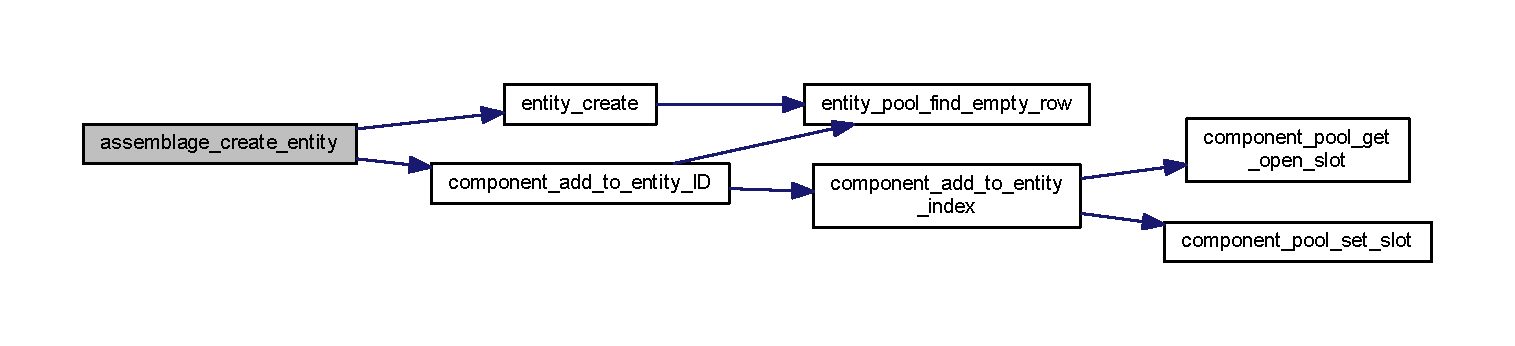
\includegraphics[width=350pt]{assemblage_8c_a8824f5dc055fa00237c2ca883a855de7_cgraph}
\end{center}
\end{figure}
\mbox{\Hypertarget{assemblage_8c_a668b0d6cb0ce05fe8b975d1549e18049}\label{assemblage_8c_a668b0d6cb0ce05fe8b975d1549e18049}} 
\index{assemblage.\+c@{assemblage.\+c}!assemblage\+\_\+register\+\_\+component@{assemblage\+\_\+register\+\_\+component}}
\index{assemblage\+\_\+register\+\_\+component@{assemblage\+\_\+register\+\_\+component}!assemblage.\+c@{assemblage.\+c}}
\subsubsection{\texorpdfstring{assemblage\+\_\+register\+\_\+component()}{assemblage\_register\_component()}}
{\footnotesize\ttfamily int assemblage\+\_\+register\+\_\+component (\begin{DoxyParamCaption}\item[{int}]{assemblage\+\_\+id,  }\item[{\mbox{\hyperlink{struct_meta_component_pool}{Meta\+Component\+Pool}} $\ast$}]{component }\end{DoxyParamCaption})}



Create a entry in the assemablage table. 


\begin{DoxyParams}{Parameters}
{\em assemblage\+\_\+id} & The assemblage id to which you wish to add the component \\
\hline
{\em component} & Pointer to the component pool that will be added to the newly created entity \\
\hline
\end{DoxyParams}
\begin{DoxyReturn}{Returns}
int Index that represents the row where the entry lives. 
\end{DoxyReturn}
Here is the call graph for this function\+:\nopagebreak
\begin{figure}[H]
\begin{center}
\leavevmode
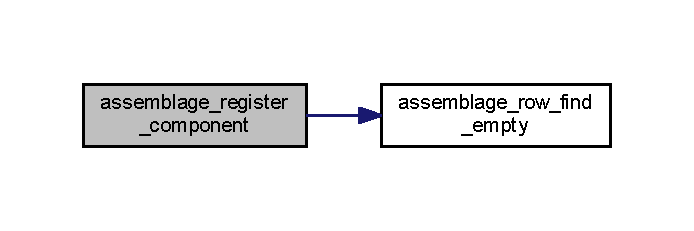
\includegraphics[width=350pt]{assemblage_8c_a668b0d6cb0ce05fe8b975d1549e18049_cgraph}
\end{center}
\end{figure}
\mbox{\Hypertarget{assemblage_8c_a075483752fba32efb629c3bf3df65279}\label{assemblage_8c_a075483752fba32efb629c3bf3df65279}} 
\index{assemblage.\+c@{assemblage.\+c}!assemblage\+\_\+remove\+\_\+component@{assemblage\+\_\+remove\+\_\+component}}
\index{assemblage\+\_\+remove\+\_\+component@{assemblage\+\_\+remove\+\_\+component}!assemblage.\+c@{assemblage.\+c}}
\subsubsection{\texorpdfstring{assemblage\+\_\+remove\+\_\+component()}{assemblage\_remove\_component()}}
{\footnotesize\ttfamily int assemblage\+\_\+remove\+\_\+component (\begin{DoxyParamCaption}\item[{int}]{assemblage\+\_\+id,  }\item[{\mbox{\hyperlink{struct_meta_component_pool}{Meta\+Component\+Pool}} $\ast$}]{component }\end{DoxyParamCaption})}



Remove a component from an assemblage. 


\begin{DoxyParams}{Parameters}
{\em assemblage\+\_\+id} & \\
\hline
{\em component} & \\
\hline
\end{DoxyParams}
\begin{DoxyReturn}{Returns}
int Error codes\+: 0 if okay, -\/1 if assemblage\+\_\+id out not in assemblage table. 
\end{DoxyReturn}
Here is the call graph for this function\+:\nopagebreak
\begin{figure}[H]
\begin{center}
\leavevmode
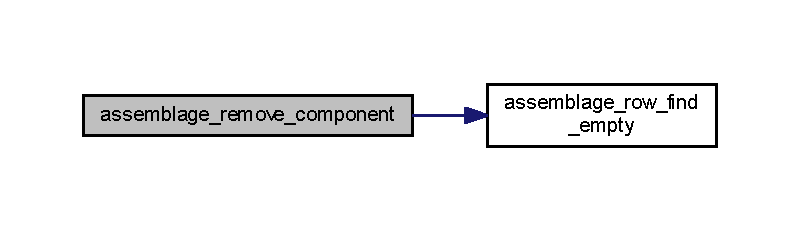
\includegraphics[width=350pt]{assemblage_8c_a075483752fba32efb629c3bf3df65279_cgraph}
\end{center}
\end{figure}
\mbox{\Hypertarget{assemblage_8c_aec35c8cc69f98525ae6406f687259673}\label{assemblage_8c_aec35c8cc69f98525ae6406f687259673}} 
\index{assemblage.\+c@{assemblage.\+c}!assemblage\+\_\+row\+\_\+find\+\_\+empty@{assemblage\+\_\+row\+\_\+find\+\_\+empty}}
\index{assemblage\+\_\+row\+\_\+find\+\_\+empty@{assemblage\+\_\+row\+\_\+find\+\_\+empty}!assemblage.\+c@{assemblage.\+c}}
\subsubsection{\texorpdfstring{assemblage\+\_\+row\+\_\+find\+\_\+empty()}{assemblage\_row\_find\_empty()}}
{\footnotesize\ttfamily int assemblage\+\_\+row\+\_\+find\+\_\+empty (\begin{DoxyParamCaption}{ }\end{DoxyParamCaption})}



Find an empty row in the assemblage table. 

\begin{DoxyReturn}{Returns}
int Index of the empty row. 
\end{DoxyReturn}
Here is the caller graph for this function\+:\nopagebreak
\begin{figure}[H]
\begin{center}
\leavevmode
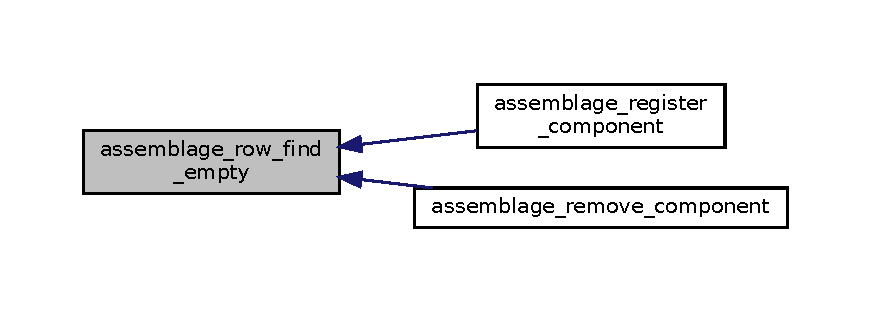
\includegraphics[width=350pt]{assemblage_8c_aec35c8cc69f98525ae6406f687259673_icgraph}
\end{center}
\end{figure}


\subsection{Variable Documentation}
\mbox{\Hypertarget{assemblage_8c_abef5ea0528d8e5d61219208774e36465}\label{assemblage_8c_abef5ea0528d8e5d61219208774e36465}} 
\index{assemblage.\+c@{assemblage.\+c}!A\+S\+S\+E\+M\+B\+L\+A\+G\+E\+\_\+\+P\+O\+OL@{A\+S\+S\+E\+M\+B\+L\+A\+G\+E\+\_\+\+P\+O\+OL}}
\index{A\+S\+S\+E\+M\+B\+L\+A\+G\+E\+\_\+\+P\+O\+OL@{A\+S\+S\+E\+M\+B\+L\+A\+G\+E\+\_\+\+P\+O\+OL}!assemblage.\+c@{assemblage.\+c}}
\subsubsection{\texorpdfstring{A\+S\+S\+E\+M\+B\+L\+A\+G\+E\+\_\+\+P\+O\+OL}{ASSEMBLAGE\_POOL}}
{\footnotesize\ttfamily \mbox{\hyperlink{struct_assemblage_pool}{Assemblage\+Pool}} A\+S\+S\+E\+M\+B\+L\+A\+G\+E\+\_\+\+P\+O\+OL}


\hypertarget{component_8c}{}\section{/home/drvanon/\+Documents/scripts/\+D\+E\+S/src/component.c File Reference}
\label{component_8c}\index{/home/drvanon/\+Documents/scripts/\+D\+E\+S/src/component.\+c@{/home/drvanon/\+Documents/scripts/\+D\+E\+S/src/component.\+c}}
{\ttfamily \#include \char`\"{}entity.\+h\char`\"{}}\newline
{\ttfamily \#include $<$stdlib.\+h$>$}\newline
Include dependency graph for component.\+c\+:\nopagebreak
\begin{figure}[H]
\begin{center}
\leavevmode
\includegraphics[width=238pt]{component_8c__incl}
\end{center}
\end{figure}
\subsection*{Functions}
\begin{DoxyCompactItemize}
\item 
\mbox{\hyperlink{struct_entity_pool}{Entity\+Pool}} $\ast$ \mbox{\hyperlink{component_8c_a67e67b5444435172378a5e24701a02e7}{entity\+\_\+get\+\_\+components}} (\mbox{\hyperlink{struct_entity_pool}{Entity\+Pool}} $\ast$entity\+\_\+pool, int guid, int max\+\_\+query\+\_\+size)
\begin{DoxyCompactList}\small\item\em Retrieve upto max\+\_\+query\+\_\+size components linked to the entity in an \mbox{\hyperlink{struct_entity_pool}{Entity\+Pool}}. \end{DoxyCompactList}\item 
\mbox{\hyperlink{struct_meta_component_pool}{Meta\+Component\+Pool}} \mbox{\hyperlink{component_8c_ac9e98c2d8d4ef8d84bda94d824fbc7b0}{component\+\_\+pool\+\_\+register}} (void $\ast$component\+\_\+pool, int size)
\begin{DoxyCompactList}\small\item\em Register a component for use in the D\+ES system. \end{DoxyCompactList}\item 
int \mbox{\hyperlink{component_8c_a997d5c45b99e95e34d3d00107eec6618}{component\+\_\+pool\+\_\+get\+\_\+open\+\_\+slot}} (\mbox{\hyperlink{struct_meta_component_pool}{Meta\+Component\+Pool}} $\ast$meta\+\_\+component\+\_\+pool)
\begin{DoxyCompactList}\small\item\em Find the first slot in the mask that has not been filled. \end{DoxyCompactList}\item 
int \mbox{\hyperlink{component_8c_a882c82b33bb428b62dab1b01c37e12a2}{component\+\_\+pool\+\_\+get\+\_\+slot}} (\mbox{\hyperlink{struct_meta_component_pool}{Meta\+Component\+Pool}} $\ast$meta\+\_\+component\+\_\+pool, int index)
\begin{DoxyCompactList}\small\item\em Find the state of a slot in a component pool. \end{DoxyCompactList}\item 
int \mbox{\hyperlink{component_8c_a1092fc1b1a8b8c021bc8e9dca328cf6c}{component\+\_\+pool\+\_\+set\+\_\+slot}} (\mbox{\hyperlink{struct_meta_component_pool}{Meta\+Component\+Pool}} $\ast$meta\+\_\+component\+\_\+pool, int index, int state)
\begin{DoxyCompactList}\small\item\em Set slot state in meta component to be vacant or free. \end{DoxyCompactList}\end{DoxyCompactItemize}


\subsection{Function Documentation}
\mbox{\Hypertarget{component_8c_a997d5c45b99e95e34d3d00107eec6618}\label{component_8c_a997d5c45b99e95e34d3d00107eec6618}} 
\index{component.\+c@{component.\+c}!component\+\_\+pool\+\_\+get\+\_\+open\+\_\+slot@{component\+\_\+pool\+\_\+get\+\_\+open\+\_\+slot}}
\index{component\+\_\+pool\+\_\+get\+\_\+open\+\_\+slot@{component\+\_\+pool\+\_\+get\+\_\+open\+\_\+slot}!component.\+c@{component.\+c}}
\subsubsection{\texorpdfstring{component\+\_\+pool\+\_\+get\+\_\+open\+\_\+slot()}{component\_pool\_get\_open\_slot()}}
{\footnotesize\ttfamily int component\+\_\+pool\+\_\+get\+\_\+open\+\_\+slot (\begin{DoxyParamCaption}\item[{\mbox{\hyperlink{struct_meta_component_pool}{Meta\+Component\+Pool}} $\ast$}]{meta\+\_\+component\+\_\+pool }\end{DoxyParamCaption})}



Find the first slot in the mask that has not been filled. 


\begin{DoxyParams}{Parameters}
{\em meta\+\_\+component\+\_\+pool} & \\
\hline
\end{DoxyParams}
\begin{DoxyReturn}{Returns}
int component index of the open slot. 
\end{DoxyReturn}
Here is the caller graph for this function\+:\nopagebreak
\begin{figure}[H]
\begin{center}
\leavevmode
\includegraphics[width=350pt]{component_8c_a997d5c45b99e95e34d3d00107eec6618_icgraph}
\end{center}
\end{figure}
\mbox{\Hypertarget{component_8c_a882c82b33bb428b62dab1b01c37e12a2}\label{component_8c_a882c82b33bb428b62dab1b01c37e12a2}} 
\index{component.\+c@{component.\+c}!component\+\_\+pool\+\_\+get\+\_\+slot@{component\+\_\+pool\+\_\+get\+\_\+slot}}
\index{component\+\_\+pool\+\_\+get\+\_\+slot@{component\+\_\+pool\+\_\+get\+\_\+slot}!component.\+c@{component.\+c}}
\subsubsection{\texorpdfstring{component\+\_\+pool\+\_\+get\+\_\+slot()}{component\_pool\_get\_slot()}}
{\footnotesize\ttfamily int component\+\_\+pool\+\_\+get\+\_\+slot (\begin{DoxyParamCaption}\item[{\mbox{\hyperlink{struct_meta_component_pool}{Meta\+Component\+Pool}} $\ast$}]{meta\+\_\+component\+\_\+pool,  }\item[{int}]{index }\end{DoxyParamCaption})}



Find the state of a slot in a component pool. 

This function will tell the user if the slot is in vacant or not.


\begin{DoxyParams}{Parameters}
{\em meta\+\_\+component\+\_\+pool} & \\
\hline
{\em index} & \\
\hline
\end{DoxyParams}
\begin{DoxyReturn}{Returns}
int bool value 
\end{DoxyReturn}
\mbox{\Hypertarget{component_8c_ac9e98c2d8d4ef8d84bda94d824fbc7b0}\label{component_8c_ac9e98c2d8d4ef8d84bda94d824fbc7b0}} 
\index{component.\+c@{component.\+c}!component\+\_\+pool\+\_\+register@{component\+\_\+pool\+\_\+register}}
\index{component\+\_\+pool\+\_\+register@{component\+\_\+pool\+\_\+register}!component.\+c@{component.\+c}}
\subsubsection{\texorpdfstring{component\+\_\+pool\+\_\+register()}{component\_pool\_register()}}
{\footnotesize\ttfamily \mbox{\hyperlink{struct_meta_component_pool}{Meta\+Component\+Pool}} component\+\_\+pool\+\_\+register (\begin{DoxyParamCaption}\item[{void $\ast$}]{component\+\_\+pool,  }\item[{int}]{size }\end{DoxyParamCaption})}



Register a component for use in the D\+ES system. 

The \mbox{\hyperlink{struct_meta_component_pool}{Meta\+Component\+Pool}} is used to provide an abstraction layer between the D\+ES and the user. It provides information on what index of the user defined component pool is open and what row is already in use by an entity. It also gives information on the size of the pool and refers to the component pool.


\begin{DoxyParams}{Parameters}
{\em component\+\_\+pool} & Pointer to the user-\/defined component\+\_\+pool. \\
\hline
{\em size} & Size of the memory allocated for the pools. \\
\hline
\end{DoxyParams}
\begin{DoxyReturn}{Returns}
\mbox{\hyperlink{struct_meta_component_pool}{Meta\+Component\+Pool}} 
\end{DoxyReturn}
Here is the caller graph for this function\+:\nopagebreak
\begin{figure}[H]
\begin{center}
\leavevmode
\includegraphics[width=297pt]{component_8c_ac9e98c2d8d4ef8d84bda94d824fbc7b0_icgraph}
\end{center}
\end{figure}
\mbox{\Hypertarget{component_8c_a1092fc1b1a8b8c021bc8e9dca328cf6c}\label{component_8c_a1092fc1b1a8b8c021bc8e9dca328cf6c}} 
\index{component.\+c@{component.\+c}!component\+\_\+pool\+\_\+set\+\_\+slot@{component\+\_\+pool\+\_\+set\+\_\+slot}}
\index{component\+\_\+pool\+\_\+set\+\_\+slot@{component\+\_\+pool\+\_\+set\+\_\+slot}!component.\+c@{component.\+c}}
\subsubsection{\texorpdfstring{component\+\_\+pool\+\_\+set\+\_\+slot()}{component\_pool\_set\_slot()}}
{\footnotesize\ttfamily int component\+\_\+pool\+\_\+set\+\_\+slot (\begin{DoxyParamCaption}\item[{\mbox{\hyperlink{struct_meta_component_pool}{Meta\+Component\+Pool}} $\ast$}]{meta\+\_\+component\+\_\+pool,  }\item[{int}]{index,  }\item[{int}]{state }\end{DoxyParamCaption})}



Set slot state in meta component to be vacant or free. 


\begin{DoxyParams}{Parameters}
{\em meta\+\_\+component\+\_\+pool} & Meta of the component pool \\
\hline
{\em index} & Index of the slot \\
\hline
{\em state} & Desired state of the slot \\
\hline
\end{DoxyParams}
\begin{DoxyReturn}{Returns}
int Error codes\+: 0 is okay, -\/1 is index out of bounds 
\end{DoxyReturn}
Here is the caller graph for this function\+:\nopagebreak
\begin{figure}[H]
\begin{center}
\leavevmode
\includegraphics[width=350pt]{component_8c_a1092fc1b1a8b8c021bc8e9dca328cf6c_icgraph}
\end{center}
\end{figure}
\mbox{\Hypertarget{component_8c_a67e67b5444435172378a5e24701a02e7}\label{component_8c_a67e67b5444435172378a5e24701a02e7}} 
\index{component.\+c@{component.\+c}!entity\+\_\+get\+\_\+components@{entity\+\_\+get\+\_\+components}}
\index{entity\+\_\+get\+\_\+components@{entity\+\_\+get\+\_\+components}!component.\+c@{component.\+c}}
\subsubsection{\texorpdfstring{entity\+\_\+get\+\_\+components()}{entity\_get\_components()}}
{\footnotesize\ttfamily \mbox{\hyperlink{struct_entity_pool}{Entity\+Pool}}$\ast$ entity\+\_\+get\+\_\+components (\begin{DoxyParamCaption}\item[{\mbox{\hyperlink{struct_entity_pool}{Entity\+Pool}} $\ast$}]{entity\+\_\+pool,  }\item[{int}]{guid,  }\item[{int}]{max\+\_\+query\+\_\+size }\end{DoxyParamCaption})}



Retrieve upto max\+\_\+query\+\_\+size components linked to the entity in an \mbox{\hyperlink{struct_entity_pool}{Entity\+Pool}}. 


\begin{DoxyParams}{Parameters}
{\em entity\+\_\+pool} & \\
\hline
{\em guid} & \\
\hline
{\em max\+\_\+query\+\_\+size} & \\
\hline
\end{DoxyParams}
\begin{DoxyReturn}{Returns}
Entity\+Pool$\ast$ 
\end{DoxyReturn}
Here is the call graph for this function\+:\nopagebreak
\begin{figure}[H]
\begin{center}
\leavevmode
\includegraphics[width=350pt]{component_8c_a67e67b5444435172378a5e24701a02e7_cgraph}
\end{center}
\end{figure}
Here is the caller graph for this function\+:\nopagebreak
\begin{figure}[H]
\begin{center}
\leavevmode
\includegraphics[width=288pt]{component_8c_a67e67b5444435172378a5e24701a02e7_icgraph}
\end{center}
\end{figure}

\hypertarget{entity_8c}{}\section{/home/drvanon/\+Documents/scripts/\+D\+E\+S/src/entity.c File Reference}
\label{entity_8c}\index{/home/drvanon/\+Documents/scripts/\+D\+E\+S/src/entity.\+c@{/home/drvanon/\+Documents/scripts/\+D\+E\+S/src/entity.\+c}}
{\ttfamily \#include $<$string.\+h$>$}\newline
{\ttfamily \#include $<$stdlib.\+h$>$}\newline
{\ttfamily \#include \char`\"{}entity.\+h\char`\"{}}\newline
Include dependency graph for entity.\+c\+:\nopagebreak
\begin{figure}[H]
\begin{center}
\leavevmode
\includegraphics[width=293pt]{entity_8c__incl}
\end{center}
\end{figure}
\subsection*{Functions}
\begin{DoxyCompactItemize}
\item 
\mbox{\hyperlink{struct_entity_pool}{Entity\+Pool}} $\ast$ \mbox{\hyperlink{entity_8c_a44b8855c1b56396b8faedcd389fe4546}{entity\+\_\+pool\+\_\+create}} (int size)
\begin{DoxyCompactList}\small\item\em Create \mbox{\hyperlink{struct_entity_pool}{Entity\+Pool}} and malloc it\textquotesingle{}s component with the size provided, returns N\+U\+LL if insufficient R\+AM. \end{DoxyCompactList}\item 
void \mbox{\hyperlink{entity_8c_a3e377867fe9b332352eb47cdf9dc1a4c}{entity\+\_\+pool\+\_\+destroy}} (\mbox{\hyperlink{struct_entity_pool}{Entity\+Pool}} $\ast$entity\+\_\+pool)
\begin{DoxyCompactList}\small\item\em Free all memory allocated for the \mbox{\hyperlink{struct_entity_pool}{Entity\+Pool}}. \end{DoxyCompactList}\item 
int \mbox{\hyperlink{entity_8c_a3955b16f45429c7ea74f275dac36493d}{entity\+\_\+pool\+\_\+find\+\_\+empty\+\_\+row}} (\mbox{\hyperlink{struct_entity_pool}{Entity\+Pool}} $\ast$entity\+\_\+pool)
\begin{DoxyCompactList}\small\item\em Find the index first empty row in the provided \mbox{\hyperlink{struct_entity_pool}{Entity\+Pool}}. \end{DoxyCompactList}\item 
int \mbox{\hyperlink{entity_8c_ae84c376a8fb9ccf53cd54e0736e76eb2}{entity\+\_\+create}} (\mbox{\hyperlink{struct_entity_pool}{Entity\+Pool}} $\ast$entity\+\_\+pool)
\begin{DoxyCompactList}\small\item\em Retrieve a new guid for an entity and register the change. \end{DoxyCompactList}\item 
int \mbox{\hyperlink{entity_8c_a45e8d15e4080e8fb930e984fc9bac47a}{component\+\_\+add\+\_\+to\+\_\+entity\+\_\+\+ID}} (\mbox{\hyperlink{struct_entity_pool}{Entity\+Pool}} $\ast$entity\+\_\+pool, int guid, \mbox{\hyperlink{struct_meta_component_pool}{Meta\+Component\+Pool}} $\ast$meta\+\_\+component\+\_\+pool)
\begin{DoxyCompactList}\small\item\em Create a new row in the component-\/entity pool. \end{DoxyCompactList}\item 
int \mbox{\hyperlink{entity_8c_a494f2d263a1053e2962e158f0a4c7e3a}{component\+\_\+add\+\_\+to\+\_\+entity\+\_\+index}} (\mbox{\hyperlink{struct_entity_pool}{Entity\+Pool}} $\ast$entity\+\_\+pool, int index, int guid, \mbox{\hyperlink{struct_meta_component_pool}{Meta\+Component\+Pool}} $\ast$meta\+\_\+component\+\_\+pool)
\begin{DoxyCompactList}\small\item\em Add a component to an entity if the user has already obtained an empty row. \end{DoxyCompactList}\item 
int \mbox{\hyperlink{entity_8c_a46ad35b10ce23dc588b43f20fa5be2c2}{component\+\_\+remove\+\_\+from\+\_\+entity\+\_\+index}} (\mbox{\hyperlink{struct_entity_pool}{Entity\+Pool}} $\ast$entity\+\_\+pool, int index)
\begin{DoxyCompactList}\small\item\em Remove the row of the given index in the component-\/entity pool. \end{DoxyCompactList}\item 
int \mbox{\hyperlink{entity_8c_af64e2220dd5596ce4f119c7887eac5c0}{component\+\_\+remove\+\_\+from\+\_\+entity\+\_\+\+ID}} (\mbox{\hyperlink{struct_entity_pool}{Entity\+Pool}} $\ast$entity\+\_\+pool, int guid, \mbox{\hyperlink{struct_meta_component_pool}{Meta\+Component\+Pool}} $\ast$meta\+\_\+component\+\_\+pool)
\begin{DoxyCompactList}\small\item\em Remove a single component from the specified entity. \end{DoxyCompactList}\item 
void \mbox{\hyperlink{entity_8c_a7fa6d71c51a14d7607b66722a1f17427}{entity\+\_\+remove}} (\mbox{\hyperlink{struct_entity_pool}{Entity\+Pool}} $\ast$entity\+\_\+pool, int guid)
\begin{DoxyCompactList}\small\item\em Remove all data on the entity in the provided \mbox{\hyperlink{struct_entity_pool}{Entity\+Pool}}. \end{DoxyCompactList}\end{DoxyCompactItemize}


\subsection{Function Documentation}
\mbox{\Hypertarget{entity_8c_a45e8d15e4080e8fb930e984fc9bac47a}\label{entity_8c_a45e8d15e4080e8fb930e984fc9bac47a}} 
\index{entity.\+c@{entity.\+c}!component\+\_\+add\+\_\+to\+\_\+entity\+\_\+\+ID@{component\+\_\+add\+\_\+to\+\_\+entity\+\_\+\+ID}}
\index{component\+\_\+add\+\_\+to\+\_\+entity\+\_\+\+ID@{component\+\_\+add\+\_\+to\+\_\+entity\+\_\+\+ID}!entity.\+c@{entity.\+c}}
\subsubsection{\texorpdfstring{component\+\_\+add\+\_\+to\+\_\+entity\+\_\+\+I\+D()}{component\_add\_to\_entity\_ID()}}
{\footnotesize\ttfamily int component\+\_\+add\+\_\+to\+\_\+entity\+\_\+\+ID (\begin{DoxyParamCaption}\item[{\mbox{\hyperlink{struct_entity_pool}{Entity\+Pool}} $\ast$}]{entity\+\_\+pool,  }\item[{int}]{guid,  }\item[{\mbox{\hyperlink{struct_meta_component_pool}{Meta\+Component\+Pool}} $\ast$}]{meta\+\_\+component\+\_\+pool }\end{DoxyParamCaption})}



Create a new row in the component-\/entity pool. 

This function takes a previously established G\+U\+ID and a \mbox{\hyperlink{struct_meta_component_pool}{Meta\+Component\+Pool}} to create a new row in the component-\/entity pool. This is to be used in combination with create\+Entity, after having registered your component. 
\begin{DoxyCode}
\textcolor{keywordtype}{int} your\_component\_pool\_size = 200; \textcolor{comment}{// Amount of rows the componentPool can have}
EnityPool *entity\_pool = \mbox{\hyperlink{examples_2velocity_2include_2des_8h_a44b8855c1b56396b8faedcd389fe4546}{entity\_pool\_create}}(2000);
MetaComponentPoolPool YourMetaComponentPoolPool = component\_register(entity\_pool, *YourComponentPool, 
      your\_component\_pool\_size);
\textcolor{keywordtype}{int} guid = \mbox{\hyperlink{examples_2velocity_2include_2des_8h_ae84c376a8fb9ccf53cd54e0736e76eb2}{entity\_create}}();
\textcolor{keywordtype}{int} component\_index = \mbox{\hyperlink{examples_2velocity_2include_2des_8h_a45e8d15e4080e8fb930e984fc9bac47a}{component\_add\_to\_entity\_ID}}(guid, &YourMetaComponentPoolPool
      );
YourComponentPool.member1[component\_index] = \textcolor{stringliteral}{"Some content"};

\textcolor{comment}{// And after running the program:}
\mbox{\hyperlink{examples_2velocity_2include_2des_8h_a3e377867fe9b332352eb47cdf9dc1a4c}{entity\_pool\_destroy}}(entity\_pool);
free(YourComponent.member1);
free(YourComponent.member2); \textcolor{comment}{// etc.}
\end{DoxyCode}



\begin{DoxyParams}{Parameters}
{\em entity\+\_\+pool} & \\
\hline
{\em guid} & \\
\hline
{\em meta\+\_\+component\+\_\+pool} & \\
\hline
\end{DoxyParams}
\begin{DoxyReturn}{Returns}
int This variable refers to the index of the user defined component pool that can be set to the prefered data, see example above. 
\end{DoxyReturn}
Here is the call graph for this function\+:\nopagebreak
\begin{figure}[H]
\begin{center}
\leavevmode
\includegraphics[width=350pt]{entity_8c_a45e8d15e4080e8fb930e984fc9bac47a_cgraph}
\end{center}
\end{figure}
Here is the caller graph for this function\+:\nopagebreak
\begin{figure}[H]
\begin{center}
\leavevmode
\includegraphics[width=350pt]{entity_8c_a45e8d15e4080e8fb930e984fc9bac47a_icgraph}
\end{center}
\end{figure}
\mbox{\Hypertarget{entity_8c_a494f2d263a1053e2962e158f0a4c7e3a}\label{entity_8c_a494f2d263a1053e2962e158f0a4c7e3a}} 
\index{entity.\+c@{entity.\+c}!component\+\_\+add\+\_\+to\+\_\+entity\+\_\+index@{component\+\_\+add\+\_\+to\+\_\+entity\+\_\+index}}
\index{component\+\_\+add\+\_\+to\+\_\+entity\+\_\+index@{component\+\_\+add\+\_\+to\+\_\+entity\+\_\+index}!entity.\+c@{entity.\+c}}
\subsubsection{\texorpdfstring{component\+\_\+add\+\_\+to\+\_\+entity\+\_\+index()}{component\_add\_to\_entity\_index()}}
{\footnotesize\ttfamily int component\+\_\+add\+\_\+to\+\_\+entity\+\_\+index (\begin{DoxyParamCaption}\item[{\mbox{\hyperlink{struct_entity_pool}{Entity\+Pool}} $\ast$}]{entity\+\_\+pool,  }\item[{int}]{index,  }\item[{int}]{guid,  }\item[{\mbox{\hyperlink{struct_meta_component_pool}{Meta\+Component\+Pool}} $\ast$}]{meta\+\_\+component\+\_\+pool }\end{DoxyParamCaption})}



Add a component to an entity if the user has already obtained an empty row. 

It is possible that the user will be aware of the row that the entity was created in, so this is a copy of add\+\_\+component\+\_\+to\+\_\+entity\+\_\+\+ID, but works based of index instead of id, which is much faster, for we will not have to go trough the entire entity pool. An example for this might be inplace replacement of a row.


\begin{DoxyParams}{Parameters}
{\em entity\+\_\+pool} & \mbox{\hyperlink{struct_entity_pool}{Entity\+Pool}} in which to perform the action. \\
\hline
{\em index} & index of the entity-\/component pool \\
\hline
{\em guid} & guid of the new entity \\
\hline
{\em meta\+\_\+component\+\_\+pool} & \mbox{\hyperlink{struct_meta_component_pool}{Meta\+Component\+Pool}} of the component that is to be added to the entity \\
\hline
\end{DoxyParams}
\begin{DoxyReturn}{Returns}
int Index of component pool that can be used to store the data the user wants to store 
\end{DoxyReturn}
Here is the call graph for this function\+:\nopagebreak
\begin{figure}[H]
\begin{center}
\leavevmode
\includegraphics[width=350pt]{entity_8c_a494f2d263a1053e2962e158f0a4c7e3a_cgraph}
\end{center}
\end{figure}
Here is the caller graph for this function\+:\nopagebreak
\begin{figure}[H]
\begin{center}
\leavevmode
\includegraphics[width=350pt]{entity_8c_a494f2d263a1053e2962e158f0a4c7e3a_icgraph}
\end{center}
\end{figure}
\mbox{\Hypertarget{entity_8c_af64e2220dd5596ce4f119c7887eac5c0}\label{entity_8c_af64e2220dd5596ce4f119c7887eac5c0}} 
\index{entity.\+c@{entity.\+c}!component\+\_\+remove\+\_\+from\+\_\+entity\+\_\+\+ID@{component\+\_\+remove\+\_\+from\+\_\+entity\+\_\+\+ID}}
\index{component\+\_\+remove\+\_\+from\+\_\+entity\+\_\+\+ID@{component\+\_\+remove\+\_\+from\+\_\+entity\+\_\+\+ID}!entity.\+c@{entity.\+c}}
\subsubsection{\texorpdfstring{component\+\_\+remove\+\_\+from\+\_\+entity\+\_\+\+I\+D()}{component\_remove\_from\_entity\_ID()}}
{\footnotesize\ttfamily int component\+\_\+remove\+\_\+from\+\_\+entity\+\_\+\+ID (\begin{DoxyParamCaption}\item[{\mbox{\hyperlink{struct_entity_pool}{Entity\+Pool}} $\ast$}]{entity\+\_\+pool,  }\item[{int}]{guid,  }\item[{\mbox{\hyperlink{struct_meta_component_pool}{Meta\+Component\+Pool}} $\ast$}]{meta\+\_\+component\+\_\+pool }\end{DoxyParamCaption})}



Remove a single component from the specified entity. 


\begin{DoxyParams}{Parameters}
{\em entity\+\_\+pool} & \\
\hline
{\em guid} & \\
\hline
{\em meta\+\_\+component\+\_\+pool} & \\
\hline
\end{DoxyParams}
\begin{DoxyReturn}{Returns}
int Error codes\+: 0 is okay, -\/1 means could not find entity-\/component in pool. 
\end{DoxyReturn}
Here is the call graph for this function\+:\nopagebreak
\begin{figure}[H]
\begin{center}
\leavevmode
\includegraphics[width=350pt]{entity_8c_af64e2220dd5596ce4f119c7887eac5c0_cgraph}
\end{center}
\end{figure}
\mbox{\Hypertarget{entity_8c_a46ad35b10ce23dc588b43f20fa5be2c2}\label{entity_8c_a46ad35b10ce23dc588b43f20fa5be2c2}} 
\index{entity.\+c@{entity.\+c}!component\+\_\+remove\+\_\+from\+\_\+entity\+\_\+index@{component\+\_\+remove\+\_\+from\+\_\+entity\+\_\+index}}
\index{component\+\_\+remove\+\_\+from\+\_\+entity\+\_\+index@{component\+\_\+remove\+\_\+from\+\_\+entity\+\_\+index}!entity.\+c@{entity.\+c}}
\subsubsection{\texorpdfstring{component\+\_\+remove\+\_\+from\+\_\+entity\+\_\+index()}{component\_remove\_from\_entity\_index()}}
{\footnotesize\ttfamily int component\+\_\+remove\+\_\+from\+\_\+entity\+\_\+index (\begin{DoxyParamCaption}\item[{\mbox{\hyperlink{struct_entity_pool}{Entity\+Pool}} $\ast$}]{entity\+\_\+pool,  }\item[{int}]{index }\end{DoxyParamCaption})}



Remove the row of the given index in the component-\/entity pool. 


\begin{DoxyParams}{Parameters}
{\em entity\+\_\+pool} & \\
\hline
{\em index} & \\
\hline
\end{DoxyParams}
\begin{DoxyReturn}{Returns}
int Error codes\+: 0 is okay, -\/1 is index out of bounds 
\end{DoxyReturn}
Here is the call graph for this function\+:\nopagebreak
\begin{figure}[H]
\begin{center}
\leavevmode
\includegraphics[width=350pt]{entity_8c_a46ad35b10ce23dc588b43f20fa5be2c2_cgraph}
\end{center}
\end{figure}
Here is the caller graph for this function\+:\nopagebreak
\begin{figure}[H]
\begin{center}
\leavevmode
\includegraphics[width=350pt]{entity_8c_a46ad35b10ce23dc588b43f20fa5be2c2_icgraph}
\end{center}
\end{figure}
\mbox{\Hypertarget{entity_8c_ae84c376a8fb9ccf53cd54e0736e76eb2}\label{entity_8c_ae84c376a8fb9ccf53cd54e0736e76eb2}} 
\index{entity.\+c@{entity.\+c}!entity\+\_\+create@{entity\+\_\+create}}
\index{entity\+\_\+create@{entity\+\_\+create}!entity.\+c@{entity.\+c}}
\subsubsection{\texorpdfstring{entity\+\_\+create()}{entity\_create()}}
{\footnotesize\ttfamily int entity\+\_\+create (\begin{DoxyParamCaption}\item[{\mbox{\hyperlink{struct_entity_pool}{Entity\+Pool}} $\ast$}]{entity\+\_\+pool }\end{DoxyParamCaption})}



Retrieve a new guid for an entity and register the change. 


\begin{DoxyParams}{Parameters}
{\em entity\+\_\+pool} & \\
\hline
\end{DoxyParams}
\begin{DoxyReturn}{Returns}
int 
\end{DoxyReturn}
Here is the call graph for this function\+:\nopagebreak
\begin{figure}[H]
\begin{center}
\leavevmode
\includegraphics[width=350pt]{entity_8c_ae84c376a8fb9ccf53cd54e0736e76eb2_cgraph}
\end{center}
\end{figure}
Here is the caller graph for this function\+:\nopagebreak
\begin{figure}[H]
\begin{center}
\leavevmode
\includegraphics[width=343pt]{entity_8c_ae84c376a8fb9ccf53cd54e0736e76eb2_icgraph}
\end{center}
\end{figure}
\mbox{\Hypertarget{entity_8c_a44b8855c1b56396b8faedcd389fe4546}\label{entity_8c_a44b8855c1b56396b8faedcd389fe4546}} 
\index{entity.\+c@{entity.\+c}!entity\+\_\+pool\+\_\+create@{entity\+\_\+pool\+\_\+create}}
\index{entity\+\_\+pool\+\_\+create@{entity\+\_\+pool\+\_\+create}!entity.\+c@{entity.\+c}}
\subsubsection{\texorpdfstring{entity\+\_\+pool\+\_\+create()}{entity\_pool\_create()}}
{\footnotesize\ttfamily \mbox{\hyperlink{struct_entity_pool}{Entity\+Pool}}$\ast$ entity\+\_\+pool\+\_\+create (\begin{DoxyParamCaption}\item[{int}]{size }\end{DoxyParamCaption})}



Create \mbox{\hyperlink{struct_entity_pool}{Entity\+Pool}} and malloc it\textquotesingle{}s component with the size provided, returns N\+U\+LL if insufficient R\+AM. 


\begin{DoxyParams}{Parameters}
{\em size} & \\
\hline
\end{DoxyParams}
\begin{DoxyReturn}{Returns}
Entity\+Pool$\ast$ 
\end{DoxyReturn}
Here is the call graph for this function\+:\nopagebreak
\begin{figure}[H]
\begin{center}
\leavevmode
\includegraphics[width=336pt]{entity_8c_a44b8855c1b56396b8faedcd389fe4546_cgraph}
\end{center}
\end{figure}
Here is the caller graph for this function\+:\nopagebreak
\begin{figure}[H]
\begin{center}
\leavevmode
\includegraphics[width=350pt]{entity_8c_a44b8855c1b56396b8faedcd389fe4546_icgraph}
\end{center}
\end{figure}
\mbox{\Hypertarget{entity_8c_a3e377867fe9b332352eb47cdf9dc1a4c}\label{entity_8c_a3e377867fe9b332352eb47cdf9dc1a4c}} 
\index{entity.\+c@{entity.\+c}!entity\+\_\+pool\+\_\+destroy@{entity\+\_\+pool\+\_\+destroy}}
\index{entity\+\_\+pool\+\_\+destroy@{entity\+\_\+pool\+\_\+destroy}!entity.\+c@{entity.\+c}}
\subsubsection{\texorpdfstring{entity\+\_\+pool\+\_\+destroy()}{entity\_pool\_destroy()}}
{\footnotesize\ttfamily void entity\+\_\+pool\+\_\+destroy (\begin{DoxyParamCaption}\item[{\mbox{\hyperlink{struct_entity_pool}{Entity\+Pool}} $\ast$}]{entity\+\_\+pool }\end{DoxyParamCaption})}



Free all memory allocated for the \mbox{\hyperlink{struct_entity_pool}{Entity\+Pool}}. 


\begin{DoxyParams}{Parameters}
{\em entity\+\_\+pool} & \\
\hline
\end{DoxyParams}
Here is the caller graph for this function\+:\nopagebreak
\begin{figure}[H]
\begin{center}
\leavevmode
\includegraphics[width=350pt]{entity_8c_a3e377867fe9b332352eb47cdf9dc1a4c_icgraph}
\end{center}
\end{figure}
\mbox{\Hypertarget{entity_8c_a3955b16f45429c7ea74f275dac36493d}\label{entity_8c_a3955b16f45429c7ea74f275dac36493d}} 
\index{entity.\+c@{entity.\+c}!entity\+\_\+pool\+\_\+find\+\_\+empty\+\_\+row@{entity\+\_\+pool\+\_\+find\+\_\+empty\+\_\+row}}
\index{entity\+\_\+pool\+\_\+find\+\_\+empty\+\_\+row@{entity\+\_\+pool\+\_\+find\+\_\+empty\+\_\+row}!entity.\+c@{entity.\+c}}
\subsubsection{\texorpdfstring{entity\+\_\+pool\+\_\+find\+\_\+empty\+\_\+row()}{entity\_pool\_find\_empty\_row()}}
{\footnotesize\ttfamily int entity\+\_\+pool\+\_\+find\+\_\+empty\+\_\+row (\begin{DoxyParamCaption}\item[{\mbox{\hyperlink{struct_entity_pool}{Entity\+Pool}} $\ast$}]{entity\+\_\+pool }\end{DoxyParamCaption})}



Find the index first empty row in the provided \mbox{\hyperlink{struct_entity_pool}{Entity\+Pool}}. 


\begin{DoxyParams}{Parameters}
{\em entity\+\_\+pool} & \\
\hline
\end{DoxyParams}
\begin{DoxyReturn}{Returns}
int 
\end{DoxyReturn}
Here is the caller graph for this function\+:\nopagebreak
\begin{figure}[H]
\begin{center}
\leavevmode
\includegraphics[width=350pt]{entity_8c_a3955b16f45429c7ea74f275dac36493d_icgraph}
\end{center}
\end{figure}
\mbox{\Hypertarget{entity_8c_a7fa6d71c51a14d7607b66722a1f17427}\label{entity_8c_a7fa6d71c51a14d7607b66722a1f17427}} 
\index{entity.\+c@{entity.\+c}!entity\+\_\+remove@{entity\+\_\+remove}}
\index{entity\+\_\+remove@{entity\+\_\+remove}!entity.\+c@{entity.\+c}}
\subsubsection{\texorpdfstring{entity\+\_\+remove()}{entity\_remove()}}
{\footnotesize\ttfamily void entity\+\_\+remove (\begin{DoxyParamCaption}\item[{\mbox{\hyperlink{struct_entity_pool}{Entity\+Pool}} $\ast$}]{entity\+\_\+pool,  }\item[{int}]{guid }\end{DoxyParamCaption})}



Remove all data on the entity in the provided \mbox{\hyperlink{struct_entity_pool}{Entity\+Pool}}. 


\begin{DoxyParams}{Parameters}
{\em entity\+\_\+pool} & \\
\hline
{\em guid} & \\
\hline
\end{DoxyParams}
Here is the call graph for this function\+:\nopagebreak
\begin{figure}[H]
\begin{center}
\leavevmode
\includegraphics[width=350pt]{entity_8c_a7fa6d71c51a14d7607b66722a1f17427_cgraph}
\end{center}
\end{figure}

\hypertarget{test_8c}{}\section{/home/drvanon/\+Documents/scripts/\+D\+E\+S/tests/test.c File Reference}
\label{test_8c}\index{/home/drvanon/\+Documents/scripts/\+D\+E\+S/tests/test.\+c@{/home/drvanon/\+Documents/scripts/\+D\+E\+S/tests/test.\+c}}
{\ttfamily \#include $<$stdio.\+h$>$}\newline
{\ttfamily \#include $<$stdlib.\+h$>$}\newline
{\ttfamily \#include \char`\"{}des.\+h\char`\"{}}\newline
Include dependency graph for test.\+c\+:\nopagebreak
\begin{figure}[H]
\begin{center}
\leavevmode
\includegraphics[width=263pt]{test_8c__incl}
\end{center}
\end{figure}
\subsection*{Data Structures}
\begin{DoxyCompactItemize}
\item 
struct \mbox{\hyperlink{struct_test_component_pool}{Test\+Component\+Pool}}
\end{DoxyCompactItemize}
\subsection*{Typedefs}
\begin{DoxyCompactItemize}
\item 
typedef struct \mbox{\hyperlink{struct_test_component_pool}{Test\+Component\+Pool}} \mbox{\hyperlink{test_8c_a21399a1be4139339f9ddb8852fa123b9}{Test\+Component\+Pool}}
\end{DoxyCompactItemize}
\subsection*{Functions}
\begin{DoxyCompactItemize}
\item 
int \mbox{\hyperlink{test_8c_ae66f6b31b5ad750f1fe042a706a4e3d4}{main}} ()
\end{DoxyCompactItemize}


\subsection{Typedef Documentation}
\mbox{\Hypertarget{test_8c_a21399a1be4139339f9ddb8852fa123b9}\label{test_8c_a21399a1be4139339f9ddb8852fa123b9}} 
\index{test.\+c@{test.\+c}!Test\+Component\+Pool@{Test\+Component\+Pool}}
\index{Test\+Component\+Pool@{Test\+Component\+Pool}!test.\+c@{test.\+c}}
\subsubsection{\texorpdfstring{Test\+Component\+Pool}{TestComponentPool}}
{\footnotesize\ttfamily typedef struct \mbox{\hyperlink{struct_test_component_pool}{Test\+Component\+Pool}}  \mbox{\hyperlink{struct_test_component_pool}{Test\+Component\+Pool}}}



\subsection{Function Documentation}
\mbox{\Hypertarget{test_8c_ae66f6b31b5ad750f1fe042a706a4e3d4}\label{test_8c_ae66f6b31b5ad750f1fe042a706a4e3d4}} 
\index{test.\+c@{test.\+c}!main@{main}}
\index{main@{main}!test.\+c@{test.\+c}}
\subsubsection{\texorpdfstring{main()}{main()}}
{\footnotesize\ttfamily int main (\begin{DoxyParamCaption}{ }\end{DoxyParamCaption})}

Here is the call graph for this function\+:\nopagebreak
\begin{figure}[H]
\begin{center}
\leavevmode
\includegraphics[width=316pt]{test_8c_ae66f6b31b5ad750f1fe042a706a4e3d4_cgraph}
\end{center}
\end{figure}

\hypertarget{tests_8h}{}\section{/home/drvanon/\+Documents/scripts/\+D\+E\+S/tests/tests.h File Reference}
\label{tests_8h}\index{/home/drvanon/\+Documents/scripts/\+D\+E\+S/tests/tests.\+h@{/home/drvanon/\+Documents/scripts/\+D\+E\+S/tests/tests.\+h}}

%--- End generated contents ---

% Index
\backmatter
\newpage
\phantomsection
\clearemptydoublepage
\addcontentsline{toc}{chapter}{Index}
\printindex

\end{document}
